\documentclass[a4paper, 11pt, openany]{book}
%
\usepackage{amsmath}
\usepackage{amssymb}
\usepackage{bbold}
\usepackage[font=bf]{caption}
\usepackage[T1]{fontenc}
\usepackage[margin=1in]{geometry}
\usepackage{graphicx}
\usepackage[colorlinks=true, allcolors=blue]{hyperref}
\usepackage[utf8]{inputenc}
\usepackage{lmodern}
\usepackage[labelformat=empty]{subfig}
\usepackage{textcomp}
%
\setcounter{tocdepth}{2}
\setcounter{secnumdepth}{2}
\setlength{\parindent}{0pt}
\setlength{\parskip}{\medskipamount}
\linespread{1.1}
\renewcommand{\floatpagefraction}{0.8}
%
\newtheorem{lemma}{Lemma}[chapter]
\newtheorem{remark}{Remark}[chapter]
\newtheorem{algorithm}{Algorithm}[chapter]
%
\newcommand*{\1}{\ensuremath{\mathbb{1}}}
\newcommand*{\R}{\ensuremath{\mathbb{R}}}
%
\title{\textbf{Technical report\\Prototype set models for supervised learning}}
\author{\Large\textcopyright\ by Nikolaus Ruf}
\date{
Python package \texttt{proset} and all associated documentation are released under the MIT software license.
See the license file in the project's git repository for details:\\
\url{https://github.com/NRuf77/proset}
}
%
\begin{document}
\maketitle
%
\pagestyle{empty}
\begin{center}
\vspace*{2in}
\Large For Shuo and Jonathan
\end{center}
\newpage
\pagestyle{plain}
%
\frontmatter
\phantomsection
\addcontentsline{toc}{chapter}{\contentsname}
\tableofcontents
%
\mainmatter
\chapter{About prototype set models}
\label{ch_about}
%
This report describes a supervised learning method we call the prototype set or `proset' algorithm.
It is an attempt to apply feature selection via the elastic net penalty to a nonlinear distribution model inspired by kernel regression.
The algorithm is implemented as Python package \texttt{proset} using an interface compatible with machine learning library \texttt{sklearn} \cite{Pedregosa_11}.\par
%
The elastic net penalty was proposed by Zou and Hastie \cite{Zou_05} as a combination of $L_1$- and $L_2$-regularization for linear regression.
Regularization with either penalty has been studied by several authors in different contexts, usually with the purpose of preventing overfitting or finding a robust solution to an ill-conditioned problem.
In case of linear regression, the name `ridge regression' for applying an $L_2$-penalty appears to be due to Hoerl and Kennard \cite{Hoerl_70}.
The LASSO algorithm that uses an $L_1$-penalty was proposed by Tibshirani \cite{Tibshirani_96}.\par
%
The main advantage of an $L_1$-penalty over an $L_2$-penalty is that its derivative does not vanish near the origin.
Thus, a sufficiently large penalty weight selects features by forcing some model coefficients exactly to zero.
The main disadvantage is that the penalty term is not differentiable at zero, which means that model fitting usually requires specialized solvers.
For example, Andrew and Gao \cite{Andrew_07} developed the OWL-QN algorithm to minimize an otherwise smooth objective function with an additional $L_1$-term.
This algorithm solves the optimization problem restricted to a particular orthant via backtracking line search.
The absolute value of each coefficient is represented as plus or minus identity depending on the orthant, so the restricted problem is everywhere differentiable.
If an optimum is found where any coefficients are exactly zero, the generalized Kuhn-Tucker conditions for the subgradient of the original term determine whether the solution is a local minimum or can be improved by moving to another orthant.
In case of proset, all model coefficients nonnegative, so optimization is naturally restricted to the first orthant.
Thus, we can rely on a standard algorithm for constrained continuous optimization like L-BFGS-B \cite{Byrd_95}.\par
%
Zou and Hastie \cite{Zou_05} show that a combined $L_1$- and $L_2$-penalty overcome some issues observed for the $L_1$-penalty applied to linear regression, but which we expect to affect other models as well.
One of these issues is that, in case of several highly correlated features, the LASSO tends to arbitrarily select only one of them.
With the elastic net penalty, highly correlated features are typically either included or excluded as a group.
Furthermore, empirical results indicate that $L_2$-regularization improves the quality of the selected models.
For these reasons and because an $L_2$-penalty does not complicate the optimization problem, we decided to use an elastic net penalty for fitting proset models.\par
%
To derive a penalized version of negative log-likelihood, we follow the approach used by Friedman, Hastie, and Tibshirani \cite{Friedman_10} for applying elastic net regularization to generalized linear models (GLMs).
This method is implemented as R package \texttt{glmnet} \cite{Friedman_10} for a variety of link functions.
In each case, a functional like this is minimized to determine model coefficients (with optional observation weights):\par
%
\begin{equation}
f_{\alpha,\lambda}\left(\beta\left|\{(x_i,y_i)\}_i\right.\right):=\frac{1}{N}\sum_{i=1}^Nl(y_i,\beta_0+\beta^Tx_i)+\lambda\left(\frac{\alpha}{2}\sum_{j=1}^d\beta_j^2+(1-\alpha)\sum_{j=1}^d|\beta_j|\right)\label{eq_regularization}
\end{equation}
%
Here, $(x_i,y_i)$ are $N\gg1$ observations with feature vectors $x_i\in\R^d$ and associated targets $y_i\in\R$, or some suitable subset thereof, e.g., the integers from $0$ to $K-1$ in case of classification with $K>1$ classes.
The link function $l$ is the negative log-likelihood for target $y_i$ conditional on a linear combination of $x_i$ with coefficients $\beta\in\R^d$ and intercept $\beta_0\in\R$.
Penalty weights $\lambda\geq0$ and $\alpha\in[0,1]$ determine the overall magnitude of the elastic net penalty and the relative importance of the $L_1$- and $L_2$-terms.
Note that the we have reversed the role of $\alpha$ compared to the formulation used in \cite{Friedman_10}, i.e., $\alpha=1$ is pure $L_2$-regularization.\par
%
Feature selection via $L_1$-penalty is a powerful technique.
It allows the user to evaluate a large number of potential input variables without having to worry about overfitting.
Unfortunately, linear regression and GLMs are limited in the achievable model quality.
As the fitting procedure only deals with feature weights in the linear combination, modeling a nonlinear relationship requires that the effect is anticipated and explicitly coded as features.
Generalized additive models (GAMs) mitigate this somewhat by automatically applying nonlinear transform to the features.
However, these transforms are restricted to a particular function class, e.g., splines with a predefined order and number of knots, and modeling higher order interactions can lead to a prohibitive number of terms.
The main reason for developing proset was to try overcoming these issues by using a different expression for the conditional distribution.\par
%
The distribution model for proset estimators is inspired by kernel-based methods from nonparametric statistics, in particular the Nadaraya-Watson estimator \cite{Nadaraya_64}\cite{Watson_64}.
This regression method uses a locally weighted average of the target values for training data to compute the conditional expectation of the target at an arbitrary point.
Let $K:\R\rightarrow\R$ be a kernel function, meaning that it is nonnegative, symmetric around the origin, and integrates to one.
Then, for any bandwidth $h>0$, $K_h(x):=\frac{1}{h}K\left(\frac{x}{h}\right)$ is also a kernel function.
Given $N$ training samples $(x_n, y_n)\in\R^2$, the Nadaraya-Watson estimator with bandwidth $h$ at $x\in\R$ is defined as
%
\begin{equation}
\hat{m}_h(x):=\frac{\sum_{n=1}^Ny_nK_h(x-x_n)}{\sum_{n=1}^NK_h(x-x_n)}\label{eq_nadaraya_watson}
\end{equation}
%
As $K_h$ goes to zero for $x\rightarrow\pm\infty$, samples where $x_n$ is close to $x$ have the most impact on $\hat{m}(x)$.
The bandwidth controls the degree of smoothing, i.e., the impact of distant points increases with $h$.
The approach can be extended to multiple features using a multivariate kernel function with positive semi-definite bandwidth matrix $H$.
Unlike GLMs or even GAMs, the Nadaraya-Watson estimator can approximate an arbitrary, smooth relationship between the features and target, as shown, e.g., by Devroye \cite{Devroye_78}.\par
%
Locally weighted averaging can also be used to estimate the conditional distribution itself instead of its expectation.
This requires replacing $y$ in (\ref{eq_nadaraya_watson}) with a kernel function centered on $y$.
A general framework that covers both continuous and discrete targets is proposed by Hall, Racine, and Li in \cite{Hall_04}.
The prototype set algorithm uses a similar approach.
A full description is given later, but two key features of proset models are:
%
\begin{itemize}
\item The bandwidth matrix is limited to a diagonal structure.
To select features, we apply an elastic-net penalty to the inverse bandwidth term for each feature.
Thus, the penalty counteracts overfitting by enforcing smoothness and removing irrelevant features from the model altogether.
%
\item Instead of including all samples with unit weight, the proset estimator includes only a subset of the training data with individual weights.
These are fitted subject to a separate elastic-net penalty term, which ensures that points are only included if they are suitably `representative' of their neighborhood.
\end{itemize}
%
We refer to the set of training points selected for a proset model as `prototypes', which is how the method gets its name.
Note that the term `prototype' has two slightly different meanings in English, both of which can be said to apply here:
%
\begin{itemize}
\item A `prototype' can be a typical example in the sense of `archetype'.
The selected samples are considered typical for their neighborhood in the feature space.
%
\item A `prototype' can be an incomplete version in the sense of `demonstrator'.
Due to feature selection, each sample included in the model is reduced to its essential features.
\end{itemize}
%
\section{Properties of proset}
\label{sec_properties}
%
The first version of the \texttt{proset} package implements a classifier -- a regressor is planned for a future release.
Chapter \ref{ch_classifier} describes the model in detail, shows how to select good hyperparameters, and provides evaluation results for several public data sets and artificial test cases.
For comparison, we also trained k-nearest-neighbor (kNN)\footnote{
The kNN method is commonly attributed to Fix and Hodges \cite{Fix_51}, although they study nonparametric density estimators for discriminatory analysis, not supervised learning.
}
and extreme gradient boosting (XGBoost) \cite{Chen_16} classifiers on the same data.
The former algorithm is conceptually close to proset as it relies on local averaging.
There is even an extension for $k=1$, Hart's `condensed nearest neighbor' algorithm \cite{Hart_68}, concerned with extracting a subset of representative points from the training data.
XGBoost has become a kind of industry standard for machine learning with highly informative features, i.e., those problems not requiring deep learning.
Empirical results shows that it is often very good at optimizing a model in terms of a chosen metric.
Both algorithms are capable of representing a nonlinear relationship between the features and target.\par
%
In the benchmark study, we optimize the models on each data set for minimal log-loss.
For the best performing algorithm, we compute the sum of cross-validation mean and standard deviation for log-loss using the optimal hyperparameters.
If another algorithm reaches a score less than or equal to this threshold, we consider it `equivalent' to the best model.
Table \ref{tab_classifier_comparison} summarizes the relative performance of the classifiers on eleven test cases.
A model is rated as either `best' (lowest log-loss), `equivalent' (log-loss less than or equal to the threshold), `worse' (log-loss above the threshold), or `worst' (classifier returns constant estimator).\par
%
\begin{table}
\caption{Comparison of classification algorithms}
\label{tab_classifier_comparison}
%
\begin{center}
\begin{tabular}{|lcccc|}
\hline
&\multicolumn{4}{c|}{\textbf{Log-loss score}}\\
\textbf{Classifier}&\textbf{Best}&\textbf{Equivalent}&\textbf{Worse}&\textbf{Worst$^*$}\\
proset&4&2&5&--\\
kNN&1&3&6&1\\
XGBoost&7&--&2&2\\
\multicolumn{5}{|l|}{$^*$ Algorithm returns constant estimator.}\\
\hline
\end{tabular}
\end{center}
\end{table}
%
For the test cases -- which are of course not representative of anything in particular -- the performance of proset is in-between kNN and XGBoost.
There are also several instances where two or all three of the models are equivalent.
The exception are three of the four cases where XGBoost is `worse' or `worst'.
These are artificial data sets where the target is a deterministic function of five or six features.
The fourth data set is very small and performance on testing data highly variable.\par
%
Our study contains artificial test cases relying on the interaction of three to six features.
XGBoost provides very good results up to four features, is worse than the other two models for five features, and fails on six features.
This may be a limitation of the binary decision trees used as base learners.
Both kNN and proset models have some predictive value for the higher order interaction terms, although results are far from perfect given that the relationship between features and target is deterministic.
If we add six more irrelevant features to the sixth order interaction, kNN also fails.
The proset classifier is able to select only the relevant inputs and produce a nontrivial estimate as before.\par
%
One particular strength of proset models we found while studying the example cases is that they tend to be highly explainable.
This is due to feature selection and that fact that the distance-based approach allows for geometric interpretation.
Another important reason is that the estimate for a particular sample tends to depend meaningfully only on a few prototypes, although the total number can go into the hundreds or thousands.
Chapter \ref{ch_explainability} `Explainability' shows examples for the following:
%
\begin{itemize}
\item Feature selection makes it easier for humans to review the model structure.
If the number of relevant features is small, users can assess whether the choice is sensible and study low-dimensional representations like scatter plots or cuts through the decision space.
%
\item Prototype selection simplifies reviewing the model structure even if the number of features is large.
We can perform weighted PCA on the feature matrix for the prototypes and use this to create low-dimensional maps of the data.
Also, a check whether the training data has labeling errors or artifacts can start with the smaller set of prototypes.
%
\item The estimate for a particular sample can be explained by reviewing the prototypes with the highest impact.
This is an explanation in terms of similar training instances instead of more abstract properties, which can help nontechnical users to understand and trust the model.
%
\item Proset rates new samples based on their absolute distance to the prototypes.
That means the algorithm can detect whether a new sample is far away from the training data and the estimate should not be relied on.
\end{itemize}
%
Note that the last three properties do not require the selected number of features to be small.
For example, proset could be used as the final stage in transfer learning and add its capabilities to a model of arbitrary complexity like a deep neural network.
%
\section{The curse of dimensionality}
\label{sec_curse}
%
The Nadaraya-Watson estimator is known to have poor convergence properties in feature spaces of high dimension.
For $n$ samples in a $d$-dimensional space, the asymptotic rate of convergence for the error is $n^{-\frac{4}{4+d}}$ \cite{Haerdle_04}.
This is due to the trade-off between the point-wise bias and variance.
Consider the simple case where $H$ is a diagonal matrix with constant bandwidth $h_n$ in each dimension.
To reduce the bias, $h_n$ has to converge to zero as $n$ goes to infinity.
To reduce the variance, the number of training points with nonnegligible impact on the estimator at any one point has to go to infinity with $n$.
As the volume containing such points is proportional to $h_n^d$, the number of points is proportional to $nh_n^d$.
Thus, the bandwidth can only converge to zero very slowly with $n$ if $d$ is large, with a corresponding slow reduction in bias.\par
%
What are the implications for proset?
Feature selection is obviously beneficial as the convergence rate of the estimator should depend only on the number of features included in the model.
The impact of prototype selection is harder to quantify.
Consider a target distribution that can be replicated exactly by proset, i.e., it is generated by local averaging using a finite number of kernel functions for weighting.
In this situation, the bandwidth does no longer have to vanish asymptotically with $n$ to yield a small bias.
We have established no theoretical results, but it would be interesting to study the convergence behavior for distributions that can be reproduced or at least closely approximated by proset.\par
%
The case with the largest dimension in the benchmark study has 2,048 features.
This is a transfer learning problem where the best results are obtained using deep neural networks.
Proset builds a model using 195 features that is worse than reference cases from literature but also not completely useless (56 \% balanced accuracy on 10 classes).
While this particular case may be overreaching, it is also considerably larger than problems that are typically considered feasible for local kernel methods.
For comparison, we found published examples with 8 features (local linear regression: Ormoneit and Hastie \cite{Ormoneit_99}),
7 to 17 features depending on the encoding of categorical variables (nonparametric conditional distribution: Bontemps, Racine, and Simoni \cite{Bontemps_09}),
or 24 variables, of which any one can serve as target (the largest sample data set for R package \texttt{np}: Hayfield and Racine \cite{Hayfield_08}).
%
\section{Release history}
\label{sec_release_history}
%
These versions of Python package \texttt{proset} have been released:
%
\begin{description}
\item[0.1.0:] implementation of proset classifier using algorithm L-BFGS-B \cite{Byrd_95} for parameter estimation;
helper functions for model fitting and plotting;
benchmark code for hyperparameter selection, comparison to other classifiers, and demonstration of explanatory features;
first version of technical report.
%
\item[0.2.0:] measures for faster computation: reduce float arrays to 32-bit precision, make solver tolerance configurable,
enable \texttt{tensorflow} \cite{Abadi_15} as alternative backend for model fitting;
reduce memory consumption for scoring;
new options for \texttt{select\_hyperparameters()}: \texttt{chunks} (macro-batching to reduce memory consumption for training), \texttt{cv\_groups} (group related samples during cross-validation);
add benchmark cases with greater sample size and feature dimension.
\end{description}
%
\endinput

\chapter{Prototype set classifier}
\label{ch_classifier}
%
In this chapter, we introduce the prototype set classifier, consider how to fit it to data, test the fitting procedure on benchmark cases, and compare model performance to other algorithms.
%
\section{Definition}
\label{sec_classifier_definition}
%
We observe $N\gg1$ i.i.d.\ pairs $(X_n,Y_n)$ of random variables such that $X_n$ takes values in $\R^D$, $D\geq1$, and $Y_n$ is one of $K>1$ classes represented by the integers from 0 to $K-1$.
Our goal is to estimate the conditional distribution of $Y_n$ given $X_n$.
As proset models are discriminative instead of generative, the distribution of $X_n$ is of no concern and we just deal with the observed realizations $x_n\in\R^D$ in practice.
Nominal or ordinal features can be included in the model via encoding as real vectors.\par
%
A proset classifier is built from $B\geq0$ ``batches'' of points selected from the available samples.
Each batch is defined by a a nonempty subset $S_1,\dots,S_B\subset\{1,\dots,N\}$ of the observation indices.
The collection of batches is denoted by
%
\begin{equation}
\mathcal{S}:=\{S_b:b\in\{1,\dots,B\}\}\label{eq_batches}
\end{equation}
%
or $\mathcal{S}=\emptyset$ if $B=0$.
The indices of each batch are $S_b=:\{s_{b,1},\dots,s_{b,J_b}\}$ where $J_b:=|S_b|$.
We refer to the samples $(x_{s_{b,j}},y_{s_{b,j}})$ as `prototypes'.
The model treats each as a representative example for the distribution of $Y_n$ when $X_n$ is in a neighborhood of $x_{s_{b,j}}$.
To make this notion more precise, we require additional notation:\par
%
The empirical marginal probabilities of $Y$ are
%
\begin{equation}
\hat{p}_{0,k}:=\frac{1}{N}\sum_{n=1}^N\1_{\{k\}}(y_k)\label{eq_p0k}
\end{equation}
%
where $\1_A$ is the indicator function of a set $A$.\par
%
The unnormalized Gaussian kernel $G_v$ with feature weights (inverse bandwidths) $v\in\R^D$, $v_d\geq0$, is
%
\begin{equation}
G_v:\R^D\rightarrow(0,1],
z\mapsto G_v(z):=\exp\left(-\frac{1}{2}\sum_{d=1}^D(v_dx_d)^2\right)\label{eq_kernel}
\end{equation}
%
We associate each batch $b$ with a vector $v_b\in\R^D$, $v_{b,d}\geq0$, and each prototype with a weight $w_{b,j}>0$ to estimate the conditional distribution as
%
\begin{equation}
P(Y=k|X=x)\approx\hat{p}_k(x):=
\frac{\hat{p}_{0,k}+\sum_{b=1}^B\sum_{j=1}^{J_b}\1_{\{k\}}(y_{s_{b,j}})w_{b,j}G_{v_b}(x-x_{s_{b,j}})}
{1+\sum_{b=1}^B\sum_{j=1}^{J_b}w_{b,j}G_{v_b}(x-x_{s_{b,j}})}
\label{eq_pkx}
\end{equation}
%
\begin{remark}
\begin{enumerate}
\item The sets $S_b$ are not required to be disjoint, so the same point can appear multiple times in (\ref{eq_pkx}).
As each batch is associated with its own $v_b$, the impact on the model may be different every time a sample appears.
%
\item We use unnormalized kernels, i.e., the integral over the kernel function is in general not equal to 1, since the scaling can be considered to be subsumed in the choice of $w_{b,j}$.
This avoids any complications related to the fact that the scaling for a Gaussian kernel depends on the number of features with nonzero coefficients.
%
\item The kernels are parameterized in terms of inverse bandwidth to enable feature selection via an $L_1$ penalty on $v_{b,d}$.
If a weight is forced to zero by the penalty, the values of the corresponding feature in points of batch $b$ cease to affect the model.
Conversely, a large value of $v_{b,d}$ means that the model is very sensitive to variations in the feature.
Kernels are limited to a diagonal bandwidth structure (product kernel) instead of a full semi-positive definite matrix to be able to fit on large feature spaces with reasonable effort.
%
\item The conditional probability (\ref{eq_pkx}) is computed as a locally weighted average similar to the Nadaraya-Watson estimator (\ref{eq_nadaraya_watson}) or the conditional distributions studied in \cite{Hall_04}.
However, there are two important differences:
%
\begin{itemize}
\item The model uses a subset of the training samples with individual weights instead of the entire data with unit weights.
This is done to reduce the computational effort for training and scoring if data size is large.
Also, studying the prototypes selected for the model may help to understand its structure.
%
\item The model adds the marginal probabilities to the contribution of the prototypes
This sets the scale for the weights $w_{b,j}$, which would otherwise be determined only up to a multiplicative constant.
Additionally, it defines a natural baseline for $B=0$ , i.e., the model that treats $Y_n$ as independent of the features.
\end{itemize}
\end{enumerate}
\end{remark}
%
Finding an optimal representation of the form (\ref{eq_pkx}) for anything but a very small sample appears intractable.
We thus focus on providing a heuristic that results in models of good quality.
The general idea is to iteratively add batches of prototypes to a base model consisting of the marginal probabilities $p_{0,k}$.
In each iteration, the available samples are split into a set of candidates for prototypes and a remainder used for scoring.
The weights for the candidates and the feature weights for the new batch are chosen to maximize a modified log-likelihood function for the scoring data.
Modifications to the likelihood are
%
\begin{enumerate}
\item reweighting the terms such that each class has the same overall weight as in the set of all samples.
This enables us to use a sampling scheme for candidates that does not draw proportionally from each class.
%
\item adding elastic net penalties for both prototype and feature weights to suppress candidates and features with negligible impact on the model.
\end{enumerate}
%
The method is greedy in so far that parameters selected during earlier iterations remain untouched.
Hyperparameters -- penalty weights and the number of batches -- are selected via cross-validation.\par
%
To state the modified likelihood and its derivatives, we make use of the following expression representing the unnormalized class probabilities truncated at batch $c\geq0$:
%
\begin{equation}
\hat{q}_{c,k}(x)=\hat{p}_{0,k}
+\sum_{b=1}^c\sum_{j=1}^{J_b}\1_{\{k\}}(y_{s_{b,j}})w_{b,j}G_{v_b}(x-x_{s_{b,j}})
\label{eq_qckx}
\end{equation}
%
These satisfy
%
\begin{align}
\hat{p}_{k}(x)&=\frac{\hat{q}_{B,k}(x)}{\sum_{l=0}^{K-1}\hat{q}_{B,l}(x)}\label{eq_q_properties}\\
\hat{q}_{0,k}(x)&=\hat{p}_{0,k}\notag\\
\forall c>0:\hat{q}_{c,k}(x)&
=\hat{q}_{c-1,k}(x)+\sum_{j=1}^{J_c}\1_{\{k\}}(y_{s_{c,j}})w_{c,j}G_{v_c}(x-x_{s_{c,j}})
\notag
\end{align}
%
During the training phase, we do not yet know the final number of batches $B$ but grow the model iteratively.
The conditional probabilities using only batches up to $c$ are given by
%
\begin{equation}
\hat{p}_{c,k}(x)=\frac{\hat{q}_{c,k}(x)}{\sum_{l=0}^{K-1}\hat{q}_{c,l}(x)}\label{eq_pckx}
\end{equation}
%
which also satisfy $\hat{p}_{0,k}(x)=\hat{p}_{0,k}$.\par
%
Given the first $c-1$ batches, the parameters for batch $c>0$ are chosen to minimize the following function, which is the negative log-likelihood with regularization as per (\ref{eq_regularization}) and reweighting as discussed above:
%
\begin{align}
f\left(v_c,\{w_{c,j}\}_j|\{x_n\}_n\right)
&=-\frac{1}{N}\sum_{k=0}^{K-1}\frac{N_k}{N_k-J_{c,k}}\sum_{n\in T_c}
\1_{\{k\}}(y_n)\log(\hat{p}_{c,k}(x_n))\label{eq_log_likelihood}\\
&+\lambda_v\left(\frac{\alpha_v}{2}\sum_{d=1}^Dv_{c,d}^2
+(1-\alpha_v)\sum_{d=1}^D|v_{c,d}|\right)\notag\\
&+\lambda_w\left(\frac{\alpha_w}{2}\sum_{j=1}^{J_c}w_{c,j}^2
+(1-\alpha_w)\sum_{j=1}^{J_c}|w_{c,j}|\right)\notag
\end{align}
%
The following expressions still need to be defined:
%
\begin{itemize}
\item $N_k:=\left|\{n\in\{1,\dots,N\}:y_n=k\}\right|$ is the number of all samples that have class $k$.
%
\item $J_{c,k}:=\left|\{j\in\{1,\dots,J_c\}:y_{s_{c,j}}=k\}\right|$
is the number of all candidates in batch $c>0$ that have class $k$.
%
\item $T_c:=\{1,\dots,N\}\setminus S_c$ is the set of samples not included as candidates for prototypes in batch $c>0$.
%
\item $\lambda_v\geq0$ is the weight for the elastic net penalty applied to feature weights.
%
\item $\lambda_w\geq0$ is the weight for the elastic net penalty applied to prototype weights.
%
\item $\alpha_v\in[0,1]$ is the portion of $\lambda_v$ assigned to the $L_2$ penalty for feature weights.
%
\item $\alpha_w\in[0,1]$ is the portion of $\lambda_w$ assigned to the $L_2$ penalty for prototype weights.
\end{itemize}
%
Given a set of prototypes $S_c$, the objective function (\ref{eq_log_likelihood}) is maximized subject to $v_{c,d}\geq0$ and $w_{c,j}\geq0$.
Note that we permit $w_{c,j}=0$ as solution of the optimization problem which contradicts our earlier definition.
However, since assigning zero weight to a point is equivalent to excluding it from the model, this does not cause any issues.\par
%
As all parameters are constrained to the first orthant, the fact that the $L_1$ penalty is not differentiable in zero does not pose a problem.
In fact, we can simply replace the absolute value with the identity function and solve the optimization task using a standard solver for continuous optimization with bounds like L-BFGS-B \cite{Byrd_95}.
%
\begin{remark}
Python package \texttt{proset} accepts optional sample weights for training.
These determine the multiplicity of an observation, e.g., a sample with weight 2.0 is treated like two separate observations with identical features.
This means that the sum of terms in (\ref{eq_log_likelihood}) is replaced by a weighted sum normalized by total weights instead of observation counts.
The marginal probabilities are also computed as weighted averages (as of package version 0.2.1).
The selection of candidates for prototypes discussed below is not affected by the weights.
\end{remark}
%
To gain the full advantage of using L-BFGS-B, we need to compute the gradient of (\ref{eq_log_likelihood}) analytically.
The partial derivatives of $\log(\hat{p}_{c,k}(x))$, $c>0$, are:
%
\begin{align}
\frac{\partial}{\partial v_{c,d}}\log(\hat{p}_{c,k}(x))&
=\frac{\frac{\partial}{\partial v_{c,d}}
\sum_{j=1}^{J_c}\1_{\{k\}}(y_{s_{c,j}})w_{c,j}G_{v_c}(x-x_{s_{c,j}})}
{\hat{q}_{c,k}(x)}
\label{eq_p_partial_v}\\
&-\frac{\frac{\partial}{\partial v_{c,d}}
\sum_{j=1}^{J_c}w_{c,j}G_{v_c}(x-x_{s_{c,j}})}
{\sum_{l=0}^{K-1}\hat{q}_{c,l}(x)}\notag\\
&=v_{c,d}\left(\frac{\sum_{j=1}^{J_c}w_{c,j}
(x_d-x_{s_{c,j},d})^2G_{v_c}(x-x_{s_{c,j}})}
{\sum_{l=0}^{K-1}\hat{q}_{c,l}(x)}\right.\notag\\
&\left.-\frac{\sum_{j=1}^{J_c}\1_{\{k\}}(y_{s_{c,j}})w_{c,j}
(x_d-x_{s_{c,j},d})^2G_{v_c}(x-x_{s_{c,j}})}
{\hat{q}_{c,k}(x)}\right)\notag\\
\frac{\partial}{\partial w_{c,i}}\log(\hat{p}_{c,k}(x))&
=\frac{\frac{\partial}{\partial w_{c,i}}
\sum_{j=1}^{J_c}\1_{\{k\}}(y_{s_{c,j}})w_{c,j}G_{v_c}(x-x_{s_{c,j}})}
{\hat{q}_{c,k}(x)}
\label{eq_p_partial_w}\\
&-\frac{\frac{\partial}{\partial w_{c,i}}
\sum_{j=1}^{J_c}w_{c,j}G_{v_c}(x-x_{s_{c,j}})}
{\sum_{l=0}^{K-1}\hat{q}_{c,l}(x)}\notag\\
&=\frac{\1_{\{k\}}(y_{s_{c,i}})G_{v_c}(x-x_{s_{c,i}})}
{\hat{q}_{c,k}(x)}
-\frac{G_{v_c}(x-x_{s_{c,i}})}
{\sum_{l=0}^{K-1}\hat{q}_{c,l}(x)}\notag
\end{align}
%
The partial derivatives of the objective function on the first orthant are
%
\begin{align}
\frac{\partial}{\partial v_{c,d}}f(v_c,\{w_{c,j}\}_j|\{x_n\}_n)
&=-\frac{1}{N}\sum_{k=0}^{K-1}\frac{N_k}{N_k-J_{c,k}}\sum_{n\in T_c}
\1_{\{k\}}(y_n)\frac{\partial}{\partial v_{c,d}}\log(\hat{p}_{c,k}(x_n))
\label{eq_l_partial_v}\\
&+\lambda(\alpha_v v_{c,d}+(1-\alpha_v))\notag\\
\frac{\partial}{\partial w_{c,j}}f(v_c,\{w_{c,j}\}_j|\{x_n\}_n)
&=-\frac{1}{N}\sum_{k=0}^{K-1}\frac{N_k}{N_k-J_{c,k}}\sum_{n\in T_c}
\1_{\{k\}}(y_n)\frac{\partial}{\partial w_{c,j}}\log(\hat{p}_{c,k}(x_n))
\label{eq_l_partial_w}\\
&+\lambda\beta(\alpha_w w_{c,j}+(1-\alpha_w))\notag
\end{align}
%
It remains to consider how to choose the prototypes for each batch and the starting points for optimization.
For the former, we score the model for iteration $c-1$ on all samples to get a probability distribution for each $Y_n$.
A sample is considered correctly classified iff the probability assigned to its true class is greater than that for the other classes.
This enables us to split the samples into $2K$ bins, i.e., the correctly and incorrectly classified samples for each class.
We now draw prototypes from these bins as evenly as possible, subject to the constraint that no bin is depleted, i.e., some samples from each bin should remain for scoring.\par
%
To make the above notion more precise, let $M>0$ be the total number of prototypes we want to consider for the new batch and $\eta\in(0,1)$ the  maximum fraction of samples we want to take from one bin.
Also, let $g_1,\dots, g_{2K}\geq0$ be the number of samples actually available in each bin, which satisfy w.l.o.g.\ $g_1\leq g_2\leq\dots\leq g_{2K}$.
To arrive at a number of samples $h_1,\dots,h_{2K}$ to draw from each bin, we use the following algorithm:
%
\begin{samepage}
\begin{algorithm}[Number of prototypes per bin]~
\label{alg_bins}
%
\begin{description}
\item{[1]} Assign $i\leftarrow1$ and $R\leftarrow M$.
%
\item{[2]} Compute $r:=\frac{R}{2K+1-i}$.
%
\item{[3]} If $r\leq\eta g_i$: assign $h_i,\dots,h_{2K}\leftarrow r$ and go to [5].
%
\item{[4]} Assign $h_i\leftarrow\eta g_i$, $i\leftarrow i+1$, $R\leftarrow R-h_i$, and go to [2].
%
\item{[5]} Round each $h_i$ to the closest integer number.
\end{description}
\end{algorithm}
\end{samepage}
%
Thus, we draw the maximum number of samples from the smallest bin that has not been processed until the remaining bins are large enough to draw an equal amount from each.
In case $\sum_{i=1}^{2K}g_i<M$,  we draw the maximum admissible number of samples from each bin.
In case $g_i\leq\frac{M}{2K}$ for all $i$, we draw an even amount $\frac{M}{2K}$ from each bin.
Note that rounding or a lack of suitable samples may mean that we do not draw exactly $M$ candidates.\par
%
\begin{remark}
This choice of sampling prototypes is motivated by the desire to give equal consideration to each class, as well as to `easy wins' -- samples that are classified correctly but could be assigned still higher probability -- and `hard cases' -- samples that are not classified correctly by the current iteration.
For a very unbalanced population, it may not be possible to treat the rare classes exactly equal to the frequent ones.
However, the rare classes are still assigned greater weight in model building than their proportion in the population.\par
%
Note also that at the start of iteration $c=1$, when the model consists only of the marginal probabilities, a sample is classified correctly iff it belongs to the most frequent class.
Thus, half of all bins are completely empty in this situation.
\end{remark}
%
In order to identify good prototypes for every class, we need to include samples from each among the candidates for prototypes and the remaining samples used for scoring. Using the proposed algorithm for distribution, the following condition is necessary and sufficient:
%
\begin{align}
&\forall k\in\{0,\dots,K-1\}:\forall n\in\{0,\dots,N_k\}:\label{eq_min_cases}\\
&(\eta n\geq0.5\vee\eta(N_k-n)\geq0.5)\wedge(\eta n<n-0.5\vee\eta(N_k-n)<N_k-n-0.5)\notag
\end{align}
%
The $n$ represents the number of samples of class $k$ that are correctly classified in iteration $c-1$.
Thus, the first clause states that the fraction $\eta$ of either the correctly or incorrectly classified cases needs to be large enough to result in a single prototype being drawn after rounding.
Likewise, the second clause states that the fraction $\eta$ of either group needs to be small enough such that at least one sample remains for scoring.\par
%
\begin{lemma}
Condition (\ref{eq_min_cases}) can be restated more compactly as
%
\begin{equation}
\forall k\in\{0,\dots,K-1\}:\lceil0.5N_k\rceil\geq0.5\eta^{-1}\wedge\lceil0.5N_k\rceil>0.5(1-\eta)^{-1}\label{eq_min_cases_2}
\end{equation}
%
where the brackets indicate rounding up.
\end{lemma}
%
\paragraph{Proof:} we show first that for any $k$ holds
%
\begin{equation}
\forall n\in\{0,\dots,N_k\}:\eta n\geq0.5\vee\eta(N_k-n)\geq0.5\iff\lceil0.5N_k\rceil\geq0.5\eta^{-1}\label{eq_condition_proof}
\end{equation}
%
The left-hand side implies the right-hand if we choose $n=\lceil0.5N_k\rceil$.\par
%
The right-hand side implies the left-hand side since for any $n$, either $n$ or $N_k-n$ has to be greater or equal to $\lceil0.5N_k\rceil$.\par
%
For the remaining clauses, note that $\eta n<n-0.5$ is equivalent to $(1-\eta)N>0.5$ so that we can use a similar argument to the one above.$\quad\Box$\par
%
A check for condition (\ref{eq_min_cases_2}) is implemented in the software to ensure that samples of each class are available both as prototypes and for scoring.
However, it does not guarantee that the algorithm is able to find meaningful structure in the data.
For example, the recommended default $\eta=0.5$ requires only that $N_k\geq3$ for all $k$, which is inadequate for supervised learning.\par
%
Regarding the starting values for optimization, we initialize all $v_{c,d}$ to $10D^{-1}$ and all $w_{c,j}$ to 1.
The former choice assumes that the features have a scale on the order of magnitude of 1, e.g., they have been scaled to unit variance.
Thus, setting the inverse bandwidth for a single feature to 10 means the kernels for the starting solution describe a structure that is more granular than the whole distribution.
Dividing the weight by the total number of features ensures that the sum of squares in the exponent of (\ref{eq_kernel}) is always of a similar magnitude and the exponential function does not vanish.
A prototype weight of 1 is of the same order of magnitude as the marginal probabilities.
%
\begin{remark}
The optimization problem does in general have multiple stationary points, including the trivial solution where all weights are equal to zero.
Provided the features are scaled, the proposed starting value for the feature weights appears to work well in practice.\par
%
Scaling the features is also recommended for a different reason.
The size of the elastic net penalty can only be interpreted relative to the scale of the partial derivatives.
Thus, to penalize all features equally, they need to be equally scaled.
\end{remark}
%
Despite regularization, there is one situation in which the selection of prototypes is not parsimonious.
If multiple candidate points have the same target and feature values for all features with positive weights, the $L_2$-penalty causes the algorithm to assign equal weight to all candidates.
If this weight is positive, the model retains multiple copies of what is effectively the same prototype (the original samples can differ in the values of excluded features).
To simplify the model representation, we add a clean-up stage to the algorithm:\par
%
Each prototype in a batch is represented by the combined vector of the active features and target.
Two prototypes are considered equivalent if the maximum norm of the difference of their associated vectors does not exceed some small tolerance.
This notion is generalized from pairs to larger groups by finding all connected components in the graph where each node represents a prototype and an edge indicates pairwise equivalence.
We then replace all prototypes belonging to the same component by a single prototype using the combined weight, as well as the features of the sample appearing first in the training data.
%
\section{Fit strategy}
\label{sec_classifier_fit}
%
Fitting a proset classifier is controlled by seven hyperparameters:
%
\begin{itemize}
\item The number of batches $B$.
%
\item The number $M$ of candidates for prototypes evaluated per batch.
%
\item The maximum fraction $\eta$ of candidates drawn from one bin using Algorithm \ref{alg_bins}.
%
\item The penalty term $\lambda_v$ for the feature weights.
%
\item The penalty term $\lambda_w$ for the prototype weights.
%
\item The ratio $\alpha_v$ of $\lambda_v$ assigned as $L_2$ penalty term.
%
\item The ratio $\alpha_w$ of $\lambda_w$ assigned as $L_2$ penalty term.
\end{itemize}
%
One goal of the case studies in this section is to identify good default values and indicate which parameters are worthwhile to tune.
Some of the key findings are summarized here:
%
\begin{enumerate}
\item Fitting a few large batches is preferable to many small ones.
The first batch has the largest impact on the model score and a large first batch results in a better overall score.
We believe the reason for this is that model quality depends on finding good constellations of prototypes, not just individual prototypes.
Suitable constellations are more likely to occur in larger batches.\par
%
Adding too many batches to a model leads to saturation, not overfitting.
The number of prototypes chosen per batch decreases, possibly down to zero.
The corresponding model scores fluctuate slightly around a common level.
Thus, using a small number of batches is mostly a question of reducing computational effort.\par
%
We recommend $M=1,000$ candidates per batch and a single batch ($B=1$) as default.
If optimizing with respect to the number of batches, $B=10$ is a reasonable upper limit.
%
\item If the number of samples in a bin is too small for drawing the desired number of candidates, a compromise is to use half of the samples as candidates and the others as reference points for computing the likelihood.
Thus, we fix $\eta=0.5$.
%
\item The penalty $\lambda_v$ for the feature weights controls the smoothness of the model.
It is the main safeguard against overfitting.\par
%
In the case study for the classifier, good values lie in the range from $10^{-6}$ to $10^{-1}$.
Choosing $10^{-3}$ as default works for all cases.
However, if an experimenter wants to tune only one parameter, it should be $\lambda_v$.
%
\item The penalty $\lambda_w$ for the prototype weights controls how much weight can be assigned to a single prototype.
We observe that increasing $\lambda_w$ within a certain range can actually lead to more candidate points being included in the model with nonzero weight.
Further increases gradually lead to underfitting.
However, reducing $\lambda_w$ does not lead to appreciable overfitting.
It appears that values below a certain threshold mostly control the preference for few prototypes with large weights versus more prototypes with smaller weights.
Above the threshold, the estimated distribution is shrunk towards the marginal probabilities.
This is desirable to some degree for avoiding overfitting.\par
%
In the case study for the classifier, good values lie in the range from $10^{-9}$ to $10^{-4}$.
Choosing $10^{-8}$ as default works for all cases.
%
\item A dominant $L_2$-penalty ($\alpha_v$ and $\alpha_w$ close to 1.0) yields slightly better results in the case study than either a dominant $L_1$- or balanced penalty.
The default values recommended for the algorithm are $\alpha_v=\alpha_w=0.95$.
\end{enumerate}
%
The case study uses the following procedure for hyperparameter search, subject to small variations described later:
%
\begin{algorithm}[Hyperparameter selection]~
\label{alg_hyperparameters}
%
\begin{enumerate}
\item Choose $M$, $\eta$, $\alpha_v$, and $\alpha_w$ based on the above recommendations.
Choose a range for $\lambda_v$, a range for $\lambda_w$, and a set of candidates for $B$ (e.g., the numbers from 0 to 10).
%
\item Split the data into a training set (70 \%) and test set (30 \%), stratified by class.
%
\item\textbf{Stage 1}
%
\begin{enumerate}
\item Randomly generate 50 pairs $(\lambda_v,\lambda_w)$.
Each $\lambda$ is sampled uniformly on the log-scale from the chosen range.
%
\item Perform five-fold cross-validation on the training set using $B=1$.
%
\item Compute the mean and standard deviation of log-loss for each pair of penalties over the left-out folds.
%
\item Determine a threshold for model quality by taking the minimal mean log-loss and adding the corresponding standard deviation.
%
\item Among all pairs whose mean log-loss is less than or equal to the threshold, choose the one maximizing the geometric mean $\sqrt{\lambda_v\lambda_w}$.
\end{enumerate}
%
\item\textbf{Stage 2}
\begin{enumerate}
\item Perform five-fold cross-validation on the training set using the parameters from stage 1 and the maximal number of batches.
%
\item For each value of $B$ up to the maximum, evaluate the models on the left-out fold and compute mean and standard deviation of log-loss.
%
\item Determine a threshold for model quality by taking the minimal mean log-loss and adding the corresponding standard deviation.
%
\item Among all candidates whose mean log-loss is less than or equal to the threshold, choose the smallest $B$.
\end{enumerate}
%
\item Refit the model with parameters selected in stages 1 and 2 on all training data.
%
\item Score the final model on the test data.
\end{enumerate}
\end{algorithm}
%
The purpose of stage 1 is to identify good values for the most important parameters $\lambda_v$ and $\lambda_w$.
Based on the observation that the first batch has the most impact, we fix $B=1$ during this stage to save computation time.
Controlling $B$ can be treated as a secondary concern, since it appears to be impossible to overfit by increasing $B$.
It is still necessary to test larger values as more complex problems may be underfitted with $B=1$.\par
%
Note that stage 2 only fits five models up to the maximum number of batches as these can also be evaluated for smaller choices of $B$.
This introduces a dependency between the means and standard deviations as estimates reuse the same initial batches.
However, as keeping $B$ small is a secondary concern, we consider this time-saving approach acceptable.\par
%
The parameters selected in each stage are not necessarily those that minimize mean cross-validation log-loss.
Instead, we consider all sets of parameters that are `equivalent' to the optimizer in the sense that their mean log-loss is within one standard error of the optimum.
From these, we pick the parameters that yield the sparsest model.
This `1 SE rule' is a recommendation from R package \texttt{glmnet} \cite{Friedman_10}.
The authors observe that a model using the optimal parameters tends to overfit the cross-validation sample, which is mitigated by the rule.
The multiplier of 1 is of course arbitrary but a common `rule of thumb' in statistics.
In case multiple parameters control sparseness, we need to decide which set we consider `sparsest'.
For stage 1, maximizing the geometric mean gives equal importance to both penalties.\par
%
As discussed in the introduction, we use the threshold obtained via the `1 SE rule' also to compare models derived via different fit strategies or classification algorithms.
For the classifier that performs best on testing data, the threshold found during stage 2 is used as upper bound on log-loss to determine which of the other classifiers are still considered `equivalent'.
%
\section{Benchmarks for hyperparameter selection}
\label{sec_classifier_benchmarks}
%
\begin{center}\fbox{\parbox{0.95\textwidth}{\small
The results in this section were generated using version 0.1.0 of Python package \texttt{proset}.
Different versions of \texttt{proset} or the underlying compute libraries may yield results that are qualitatively similar but not identical.
}}\end{center}
%
In this section, we test variations of the fit strategy outlined above on different benchmark cases.
We use four small data sets that come as `toy' examples with Python package \texttt{sklearn} \cite{Pedregosa_11}, plus two slightly larger artificial data sets:
%
\begin{enumerate}
\item\textbf{Iris 2f:} this data set consists of the first two features of Fisher's famous iris data set \cite{Fisher_36}.
We limit the analysis to two of four features (sepal length and width) as this allows us to visualize the decision surface of the classifier as a 2d plot.
The data set comprises 150 samples for three species of iris flower, with 50 samples per class.
One class is linearly separable from the others, but measurements for the remaining two overlap.
%
\item\textbf{Wine:} this data set from the  UCI Machine Learning Repository \cite{Dua_19} consists of chemical analysis data for wines from three different cultivators.
It consists of 178 samples with between 48 and 71 samples per class.
The data is known to be separable \cite{Aeberhard_92}.
%
\item\textbf{Cancer:} this data set from the UCI Machine Learning Repository \cite{Dua_19} consists of medical analysis data from breast tissue samples.
The 569 samples are classified as either malignant (212 samples) or benign (357 samples).
%
\item\textbf{Digits:} this data set from the UCI Machine Learning Repository \cite{Dua_19} consists of greyscale images of handwritten digits downsampled to an eight-by-eight grid.
The 1,797 samples are approximately balanced among the 10 digits.
%
\item\textbf{Checker:} for this artificial data set, we sample two features uniformly on the unit square and assign class labels deterministically to create an eight-by-eight checkerboard.
The pattern defeats methods that rely on global properties of the data like correlation, e.g., logistic regression.
It can be recovered successfully by methods that model local structure, e.g., a k-nearest neighbor classifier or decision tree.
The total number of samples is 6,400, so each square of the pattern contains approximately 100 data points.
%
\item\textbf{XOR 6f:} for this artificial data set, we sample six features independently and uniformly on the interval $[-1.0, 1.0]$.
The class label is assigned deterministically based on the sign of the product of features: a positive (or zero) sign is class 1, a negative sign is class 0.
This is similar to the `continuous XOR' problem found in the \texttt{mlbench} library for R \cite{Leisch_21}, except that we only distinguish two classes.
Despite being deterministic, this problem appears to be a hard even for classifiers that model local structure.
The number of samples is 6,400, so each orthant of the feature space contains approximately 100 data points.
\end{enumerate}
%
Features for all benchmark data sets are centered and scaled before fitting a proset model.\par
%
The first three experiments consider the impact of $\alpha_v$ and $\alpha_w$ on model behavior.
Proset classifiers are fitted to all six data sets with fixed $M=1,000$ and $\eta=0.5$.
Penalty weights are sampled from the ranges $\lambda_v\in(10^{-6},10^{-1})$ and $\lambda_w\in(10^{-9},10^{-4})$, while the number of batches is allowed to vary between 0 and 10.
The first experiment uses a dominant $L_1$-penalty ($\alpha_v=\alpha_w=0.05$), the second uses balanced penalties ($\alpha_v=\alpha_w=0.50$), and the third a dominant $L_2$-penalty ($\alpha_v=\alpha_w=0.95$).\par
%
\begin{figure}
\caption{[E1] Parameter search for Iris 2F data}
\label{fig_parameter_search}
%
\begin{center}
\subfloat[\textbf{Stage 1}]{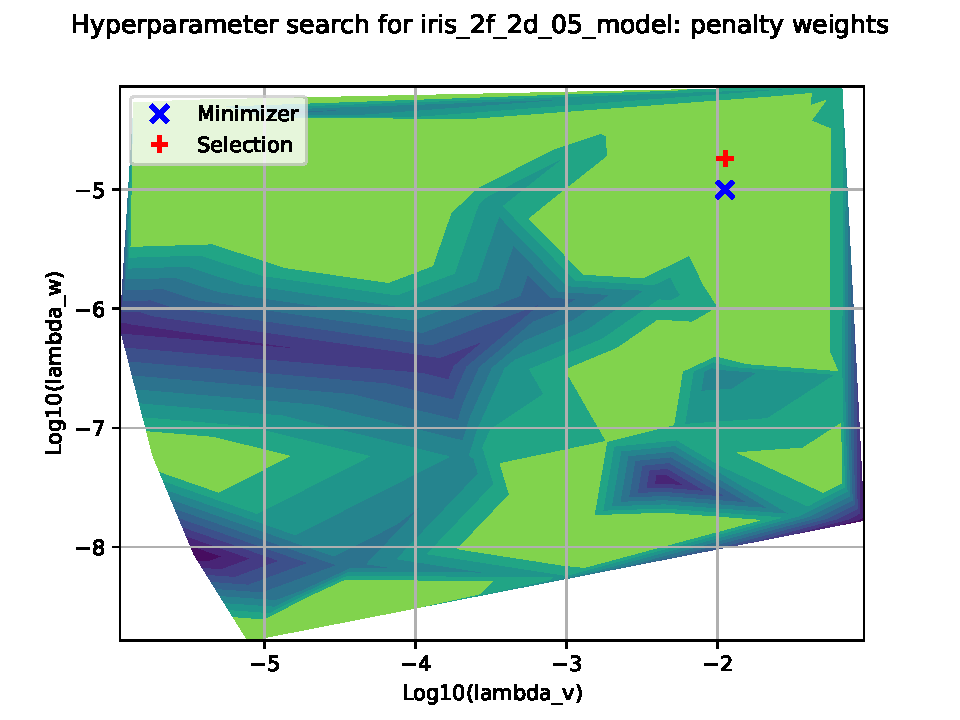
\includegraphics[height=0.4\textheight]{figures/iris_2f_dominant_l1_2d_search.pdf}}\\
\subfloat[\textbf{Both stages}]{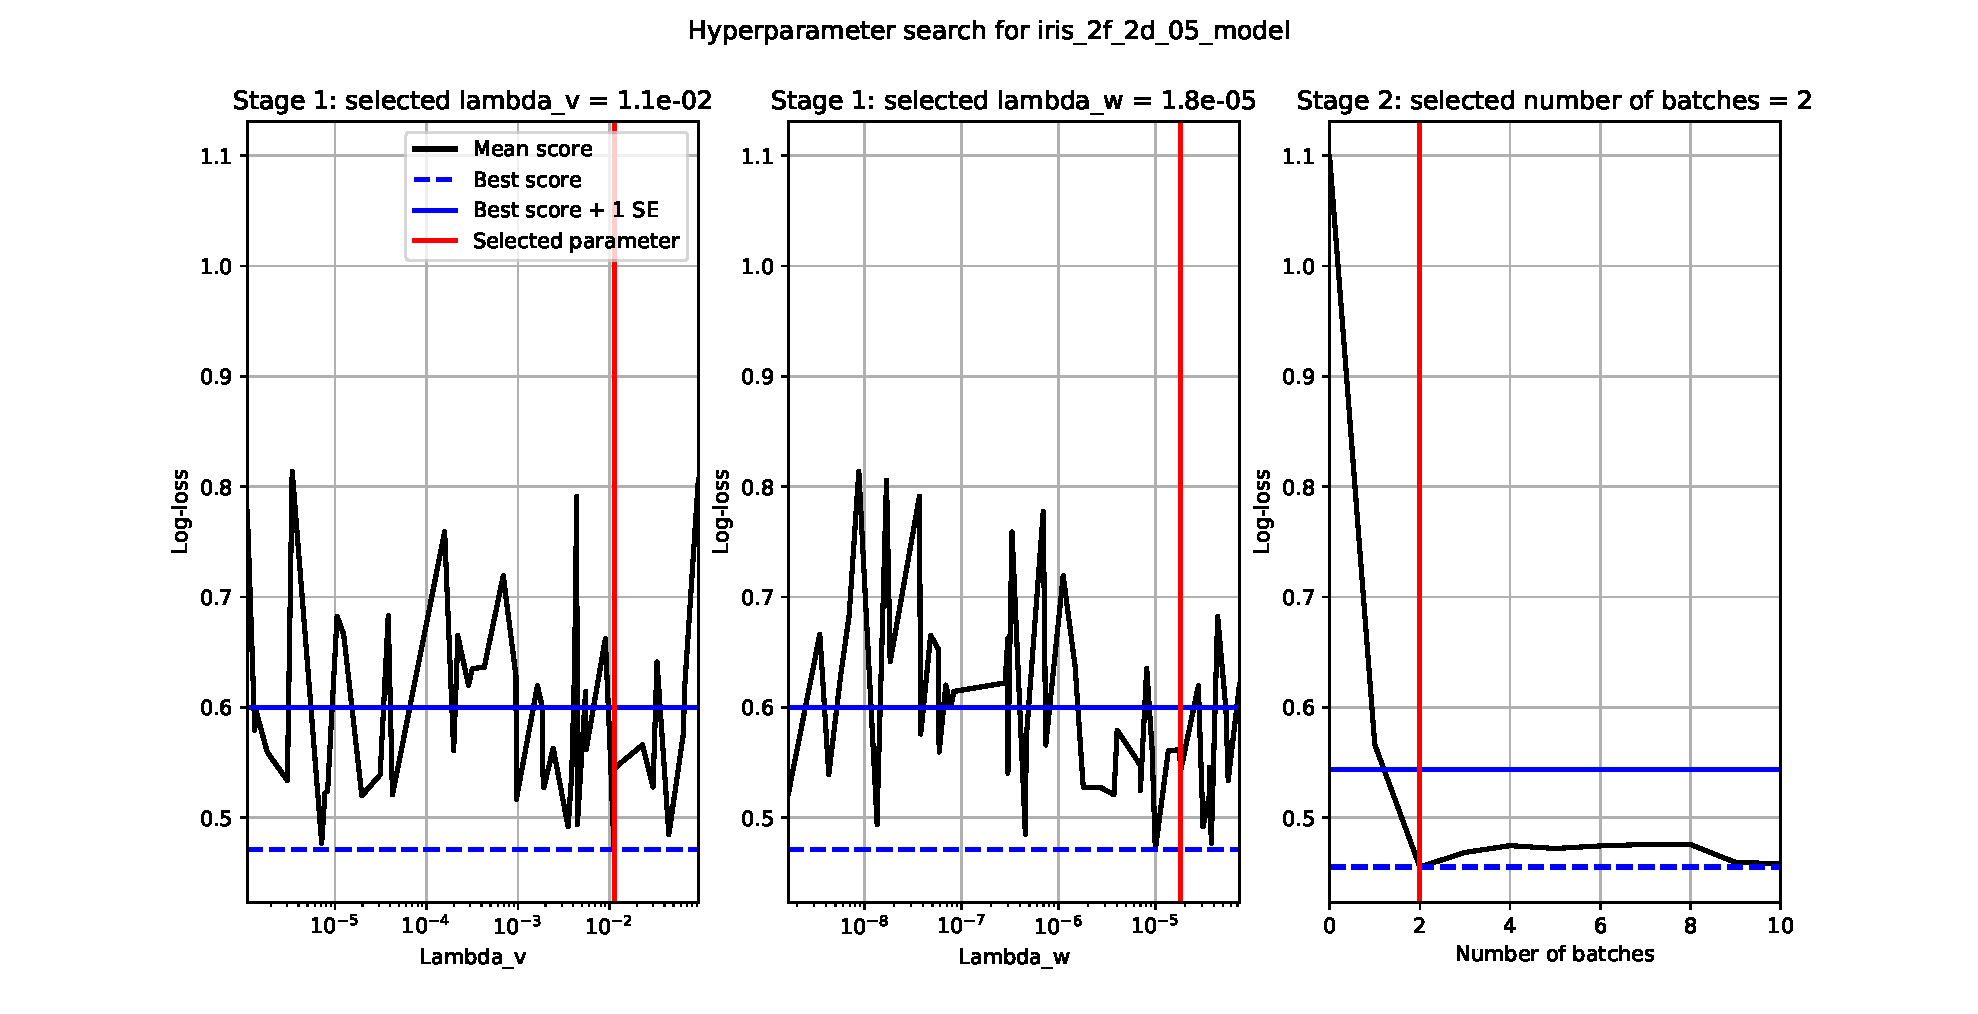
\includegraphics[width=0.99\textwidth, trim={0.5cm 0.5cm 0.5cm 0.5cm}, clip]{figures/iris_2f_dominant_l1_1d_search.pdf}}
\end{center}
\end{figure}
%
Figure \ref{fig_parameter_search} shows parameter search results for the first experiment using iris data.
In the lower plot, the log-loss for stage 1 as a function of either $\lambda_v$ or $\lambda_w$ appears highly variable.
However, this is mostly due to changes in the other parameter, as evidenced by the surface plot.
Complete results for all data sets are presented in Tables \ref{tab_e1}, \ref{tab_e2}, and \ref{tab_e3}.
A comparison of the first six experiments is found in Table \ref{tab_e1_to_e6}.
The description of individual experiments comprises the following information:
%
\begin{description}
\item[Data:] the number of classes, as well as the size of the whole data set and train-test split.
%
\item[Candidates:] the approximate number of candidates for prototypes used to build the final model.
While $M=1,000$ candidates are specified for each model, the effective maximum for small data sets is around 35 \% of the available samples: training data is 70 \% of all samples and $\eta=0.5$ allows at most 50 \% of data in one bin to be used as prototypes.
%
\item[Stage 1:] results for selecting $\lambda_v$ and $\lambda_w$ using a single batch.
Lists the optimal and chosen parameters according to the `1 SE rule' (see algorithm \ref{alg_hyperparameters}), together with the achieved mean log-loss from cross-validation.
The given threshold is the one for the `1 SE rule', i.e., the sum of the minimal mean log-loss and corresponding standard deviation.
%
\item[Stage 2:] results for selecting $B$ using the penalty weights chosen in stage 1.
%
\item[Final model:] information about the final model fitted on all training data with parameters determined in stages 1 and 2.
The number of features and prototypes, as well as the scores achieved for the test data.
Apart from log-loss, the measures used for evaluation are ROC-AUC and balanced accuracy.\par
%
For multi-class problems, the stated ROC-AUC values is the unweighted average for all pairwise comparisons of two classes.
This generalization to more than two classes is recommended in \cite{Hand_01} as being robust to class imbalance.\par
%
To compute balanced accuracy, we use the `naive' rule that assigns each sample the class label with the highest estimated probability.
The reported score is the unweighted average of the correct classification rates for each class.
\end{description}
%
\begin{table}
\caption{[E1] Randomized search for $\lambda_v$ and $\lambda_w$ ($\alpha_v=\alpha_w=0.05$)}
\label{tab_e1}
%
\begin{center}
\small
\begin{tabular}{|lrrrrrr|}
\hline
&\multicolumn{6}{c|}{\textbf{\hrulefill\ Data set \hrulefill}}\\
&\textbf{Iris 2f}&\textbf{Wine}&\textbf{Cancer}&\textbf{Digits}&\textbf{Checker}&\textbf{XOR 6f}\\
\multicolumn{7}{|l|}{\textbf{Data}}\\
Classes&3&3&2&10&2&2\\
Features&2&13&30&64&2&6\\
Samples&150&178&569&1,797&6,400&6,400\\
Train samples&105&124&398&1,257&4,480&4,480\\
Test samples&45&54&171&540&1,920&1,920\\
\textbf{Candidates}&$\sim50$&$\sim60$&$\sim200$&$\sim630$&1,000&1,000\\
\multicolumn{7}{|l|}{\textbf{Stage 1}}\\
Optimal $\lambda_v$&$1.1\times10^{-2}$&$6.9\times10^{-4}$&$5.5\times10^{-3}$&$1.2\times10^{-5}$&$4.5\times10^{-3}$&$1.0\times10^{-2}$\\
Selected $\lambda_v$&$1.1\times10^{-2}$&$3.5\times10^{-3}$&$1.1\times10^{-2}$&$1.8\times10^{-3}$&$5.5\times10^{-3}$&$1.1\times10^{-2}$\\
Optimal $\lambda_w$&$1.0\times10^{-5}$&$1.1\times10^{-6}$&$8.3\times10^{-8}$&$3.4\times10^{-9}$&$1.3\times10^{-8}$&$4.6\times10^{-7}$\\
Selected $\lambda_w$&$1.8\times10^{-5}$&$3.1\times10^{-5}$&$1.8\times10^{-5}$&$7.7\times10^{-8}$&$8.3\times10^{-8}$&$1.0\times10^{-5}$\\
Optimal log-loss&0.47&0.12&0.09&0.16&0.17&0.53\\
Threshold&0.60&0.17&0.14&0.19&0.18&0.55\\
Selected log-loss&0.54&0.12&0.09&0.19&0.18&0.55\\
\multicolumn{7}{|l|}{\textbf{Stage 2}}\\
Optimal batches&2&5&1&9&1&1\\
Selected batches&2&2&1&1&1&1\\
Optimal log-loss&0.46&0.12&0.10&0.18&0.19&0.55\\
Threshold&0.54&0.16&0.14&0.22&0.20&0.56\\
Selected log-loss&0.46&0.13&0.10&0.19&0.19&0.55\\
\multicolumn{7}{|l|}{\textbf{Final model, scores for test data}}\\
Active features&2&6&3&19&2&6\\
Prototypes&34&43&24&546&257&309\\
Log-loss&0.62&0.14&0.13&0.15&0.17&0.55\\
ROC-AUC&0.86&0.99&0.99&1.00&0.99&0.81\\
Balanced acc.&0.76&0.97&0.94&0.97&0.95&0.71\\
\hline
\end{tabular}
\end{center}
\end{table}
%
\begin{table}
\caption{[E2] Randomized search for $\lambda_v$ and $\lambda_w$ ($\alpha_v=\alpha_w=0.50$)}
\label{tab_e2}
%
\begin{center}
\small
\begin{tabular}{|lrrrrrr|}
\hline
&\multicolumn{6}{c|}{\textbf{\hrulefill\ Data set \hrulefill}}\\
&\textbf{Iris 2f}&\textbf{Wine}&\textbf{Cancer}&\textbf{Digits}&\textbf{Checker}&\textbf{XOR 6f}\\
\multicolumn{7}{|l|}{\textbf{Data}}\\
Classes&3&3&2&10&2&2\\
Features&2&13&30&64&2&6\\
Samples&150&178&569&1,797&6,400&6,400\\
Train samples&105&124&398&1,257&4,480&4,480\\
Test samples&45&54&171&540&1,920&1,920\\
\textbf{Candidates}&$\sim50$&$\sim60$&$\sim200$&$\sim630$&1,000&1,000\\
\multicolumn{7}{|l|}{\textbf{Stage 1}}\\
Optimal $\lambda_v$&$5.6\times10^{-3}$&$1.0\times10^{-2}$&$5.5\times10^{-3}$&$1.2\times10^{-5}$&$9.5\times10^{-4}$&$5.5\times10^{-3}$\\
Selected $\lambda_v$&$1.1\times10^{-2}$&$3.5\times10^{-3}$&$1.1\times10^{-2}$&$4.5\times10^{-3}$&$9.5\times10^{-4}$&$1.0\times10^{-2}$\\
Optimal $\lambda_w$&$1.7\times10^{-5}$&$4.6\times10^{-7}$&$8.3\times10^{-8}$&$3.4\times10^{-9}$&$5.6\times10^{-9}$&$8.3\times10^{-8}$\\
Selected $\lambda_w$&$1.0\times10^{-5}$&$3.1\times10^{-5}$&$1.8\times10^{-5}$&$1.3\times10^{-8}$&$5.6\times10^{-9}$&$4.6\times10^{-7}$\\
Optimal log-loss&0.45&0.10&0.09&0.17&0.17&0.53\\
Threshold&0.51&0.17&0.14&0.20&0.17&0.54\\
Selected log-loss&0.46&0.13&0.09&0.19&0.17&0.54\\
\multicolumn{7}{|l|}{\textbf{Stage 2}}\\
Optimal batches&4&10&1&3&1&1\\
Selected batches&3&2&1&1&1&1\\
Optimal log-loss&0.46&0.13&0.10&0.16&0.18&0.54\\
Threshold&0.49&0.16&0.14&0.19&0.19&0.55\\
Selected log-loss&0.47&0.14&0.10&0.18&0.18&0.54\\
\multicolumn{7}{|l|}{\textbf{Final model, scores for test data}}\\
Active features&2&7&3&18&2&6\\
Prototypes&30&69&54&533&281&360\\
Log-loss&0.49&0.20&0.13&0.18&0.16&0.53\\
ROC-AUC&0.90&0.98&0.99&1.00&0.99&0.82\\
Balanced acc.&0.73&0.93&0.95&0.97&0.95&0.72\\
\hline
\end{tabular}
\end{center}
\end{table}
%
\begin{table}
\caption{[E3] Randomized search for $\lambda_v$ and $\lambda_w$ ($\alpha_v=\alpha_w=0.95$)}
\label{tab_e3}
%
\begin{center}
\small
\begin{tabular}{|lrrrrrr|}
\hline
&\multicolumn{6}{c|}{\textbf{\hrulefill\ Data set \hrulefill}}\\
&\textbf{Iris 2f}&\textbf{Wine}&\textbf{Cancer}&\textbf{Digits}&\textbf{Checker}&\textbf{XOR 6f}\\
\multicolumn{7}{|l|}{\textbf{Data}}\\
Classes&3&3&2&10&2&2\\
Features&2&13&30&64&2&6\\
Samples&150&178&569&1,797&6,400&6,400\\
Train samples&105&124&398&1,257&4,480&4,480\\
Test samples&45&54&171&540&1,920&1,920\\
\textbf{Candidates}&$\sim50$&$\sim60$&$\sim200$&$\sim630$&1,000&1,000\\
\multicolumn{7}{|l|}{\textbf{Stage 1}}\\
Optimal $\lambda_v$&$5.6\times10^{-3}$&$3.8\times10^{-5}$&$5.5\times10^{-3}$&$7.8\times10^{-6}$&$3.1\times10^{-5}$&$5.5\times10^{-3}$\\
Selected $\lambda_v$&$1.1\times10^{-2}$&$1.1\times10^{-2}$&$1.1\times10^{-2}$&$9.5\times10^{-4}$&$2.9\times10^{-4}$&$5.5\times10^{-3}$\\
Optimal $\lambda_w$&$1.7\times10^{-5}$&$6.9\times10^{-9}$&$8.3\times10^{-8}$&$1.6\times10^{-9}$&$4.3\times10^{-9}$&$8.3\times10^{-8}$\\
Selected $\lambda_w$&$1.0\times10^{-5}$&$1.8\times10^{-5}$&$1.8\times10^{-5}$&$5.6\times10^{-9}$&$6.9\times10^{-8}$&$8.3\times10^{-8}$\\
Optimal log-loss&0.44&0.11&0.09&0.17&0.18&0.53\\
Threshold&0.49&0.18&0.14&0.19&0.20&0.54\\
Selected log-loss&0.46&0.17&0.11&0.18&0.19&0.53\\
\multicolumn{7}{|l|}{\textbf{Stage 2}}\\
Optimal batches&5&5&1&8&1&10\\
Selected batches&3&2&1&2&1&1\\
Optimal log-loss&0.51&0.14&0.10&0.14&0.19&0.51\\
Threshold&0.57&0.17&0.14&0.17&0.20&0.53\\
Selected log-loss&0.56&0.15&0.10&0.16&0.19&0.53\\
\multicolumn{7}{|l|}{\textbf{Final model, scores for test data}}\\
Active features&2&7&4&30&2&6\\
Prototypes&49&52&56&861&328&413\\
Log-loss&0.43&0.14&0.13&0.15&0.18&0.52\\
ROC-AUC&0.91&1.00&0.99&1.00&0.99&0.82\\
Balanced acc.&0.71&0.98&0.98&0.97&0.95&0.72\\
\hline
\end{tabular}
\end{center}
\end{table}
%
\clearpage
%
In the experiments, a dominant $L_1$-penalty yields slightly worse results than balanced penalties or a dominant $L_2$-penalty.
Also, we have occasionally observed (not in the results reported here) that a dominant $L_1$-penalty causes too few features to be selected for the final model.
This happens even though models created during cross-validation do not underfit.
The likely reason is that random candidate selection for small sample size can result in a set of candidates hat does not fully represent the data.
Since a dominant $L_2$-penalty slightly outperforms the balanced case in the trials, we recommend $\alpha_v=\alpha_w=0.95$ as default values.\par
%
\begin{table}
\caption{[E4] Use optimal hyperparameters ($\alpha_v=\alpha_w=0.95$)}
\label{tab_e4}
%
\begin{center}
\small
\begin{tabular}{|lrrrrrr|}
\hline
&\multicolumn{6}{c|}{\textbf{\hrulefill\ Data set \hrulefill}}\\
&\textbf{Iris 2f}&\textbf{Wine}&\textbf{Cancer}&\textbf{Digits}&\textbf{Checker}&\textbf{XOR 6f}\\
\multicolumn{7}{|l|}{\textbf{Data}}\\
Classes&3&3&2&10&2&2\\
Features&2&13&30&64&2&6\\
Samples&150&178&569&1,797&6,400&6,400\\
Train samples&105&124&398&1,257&4,480&4,480\\
Test samples&45&54&171&540&1,920&1,920\\
\textbf{Candidates}&$\sim50$&$\sim60$&$\sim200$&$\sim630$&1,000&1,000\\
\multicolumn{7}{|l|}{\textbf{Stage 1}}\\
Optimal $\lambda_v$&$5.6\times10^{-3}$&$3.8\times10^{-5}$&$5.5\times10^{-3}$&$7.8\times10^{-6}$&$3.1\times10^{-5}$&$5.5\times10^{-3}$\\
Optimal $\lambda_w$&$1.7\times10^{-5}$&$6.9\times10^{-9}$&$8.3\times10^{-8}$&$1.6\times10^{-9}$&$4.3\times10^{-9}$&$8.3\times10^{-8}$\\
Optimal log-loss&0.44&0.11&0.09&0.17&0.18&0.53\\
Threshold&0.49&0.18&0.14&0.19&0.20&0.54\\
\multicolumn{7}{|l|}{\textbf{Stage 2}}\\
Optimal batches&5&5&1&8&1&10\\
Optimal log-loss&0.51&0.14&0.10&0.14&0.19&0.51\\
Threshold&0.57&0.17&0.14&0.17&0.20&0.53\\
\multicolumn{7}{|l|}{\textbf{Final model, scores for test data}}\\
Active features&2&11&3&41&2&6\\
Prototypes&65&204&93&3,053&595&403\\
Log-loss&0.48&0.05&0.11&0.13&0.16&0.52\\
ROC-AUC&0.87&1.00&0.99&1.00&0.99&0.83\\
Balanced acc.&0.69&0.98&0.95&0.97&0.94&0.74\\
\hline
\end{tabular}
\end{center}
\end{table}
%
The fourth experiment shows the effect of using the optimal parameters from cross-validation instead of the equivalent sparser solution (see Table \ref{tab_e4}).
In half of the cases, results actually outperform those of the first three experiments.
However, the log-loss scores for [E3] are still below the equivalence thresholds for [E4] in these cases.
This means the metrics for the benchmark cases do not indicate that the `1 SE rule' is necessary to prevent overfitting, but we can use it to obtain a sparser parameterization with negligible loss in quality.
%
\clearpage
%
\begin{figure}
\caption{Proset decision surfaces for case Iris 2f}
\label{fig_proset_decision_iris_2f}
%
\begin{center}
\subfloat[\textbf{[E1] $\lambda_v=\lambda_w=0.05$, `1 SE rule'}]{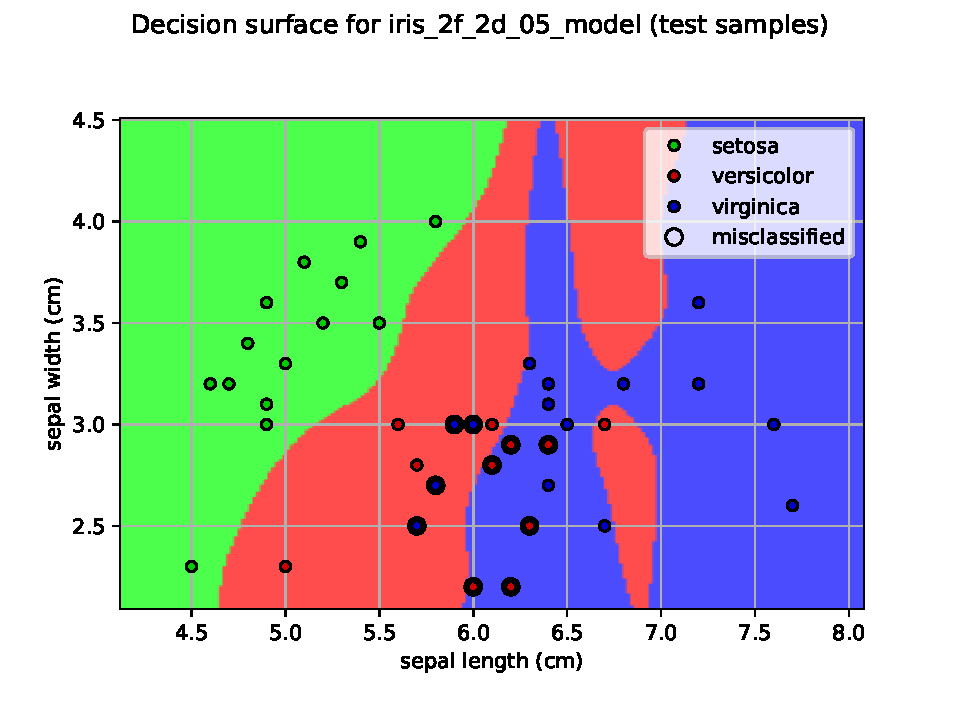
\includegraphics[width=0.49\textwidth]{figures/iris_2f_dominant_l1_surf_test.pdf}}
\subfloat[\textbf{[E2] $\lambda_v=\lambda_w=0.50$, `1 SE rule'}]{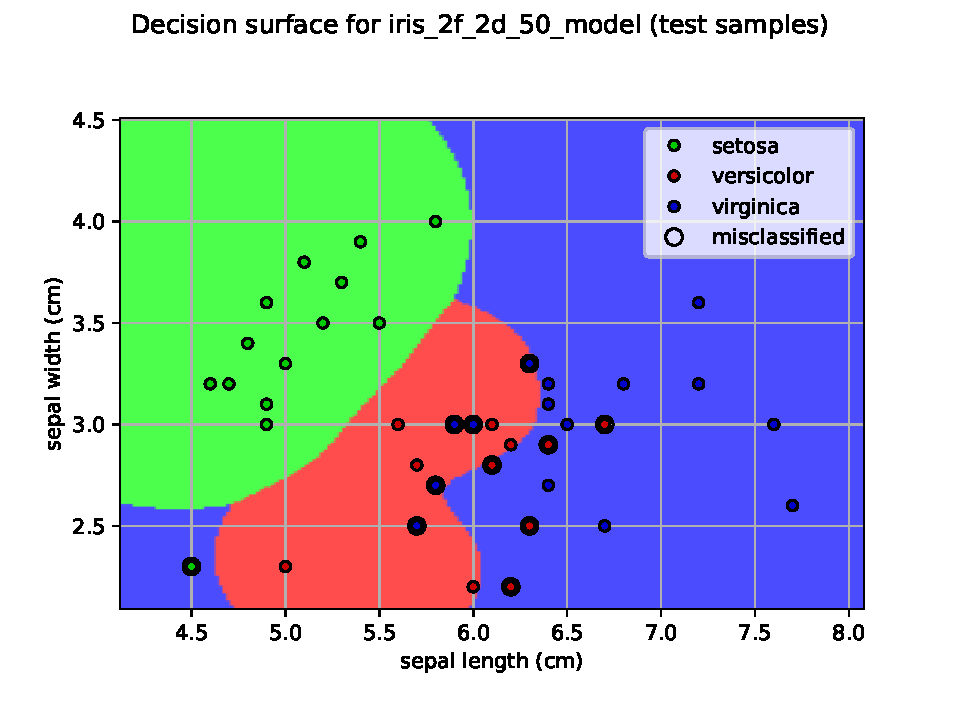
\includegraphics[width=0.49\textwidth]{figures/iris_2f_balanced_surf_test.pdf}}\\
\subfloat[\textbf{[E3] $\lambda_v=\lambda_w=0.95$, `1 SE rule'}]{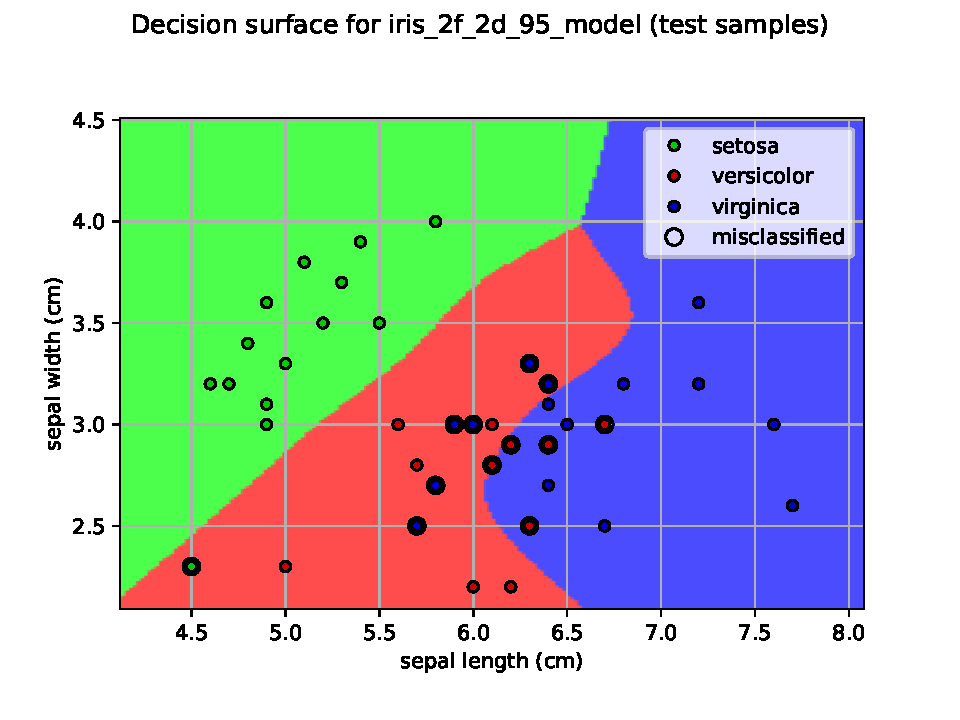
\includegraphics[width=0.49\textwidth]{figures/iris_2f_dominant_l2_surf_test.pdf}}
\subfloat[\textbf{[E4] $\lambda_v=\lambda_w=0.95$, optimal hyperparameters}]{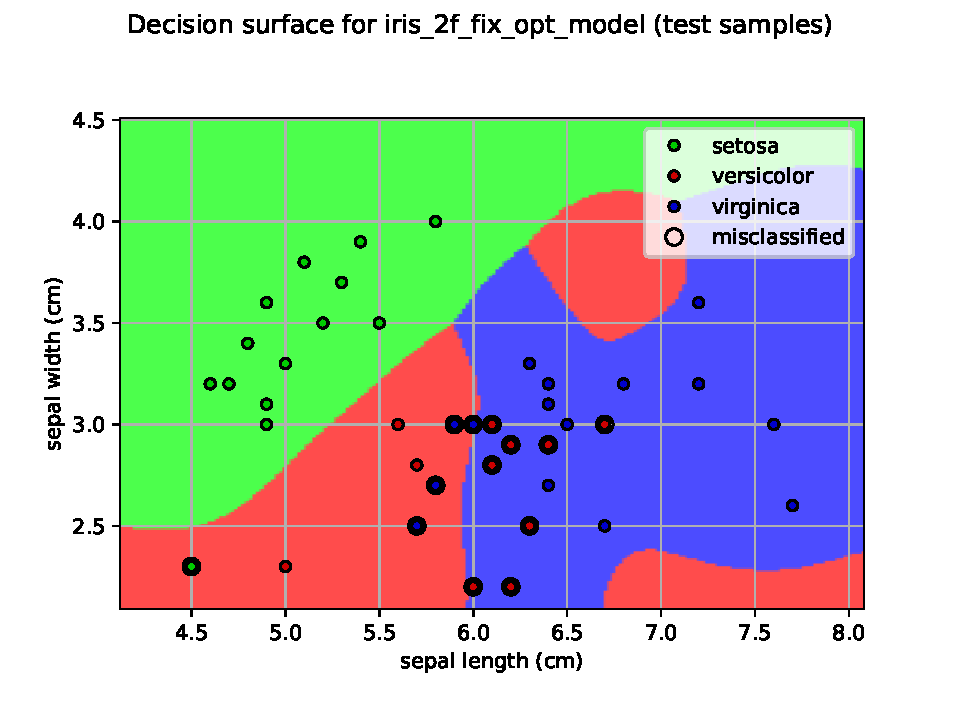
\includegraphics[width=0.49\textwidth]{figures/iris_2f_dominant_l2_surf_opt_test.pdf}}
\end{center}
\end{figure}
%
If we study the decision surfaces for the Iris 2f benchmark, it does look like [E4] has a slight tendency to overfit.
Figure \ref{fig_proset_decision_iris_2f} shows the surface plots for experiments [E1] to [E4].
The colors indicates the class with the highest estimated probability in that region of the feature space.
Only the result for [E3] appears fully convincing to us.
It separates the feature space near the training data into three contiguous regions with smooth boundaries.
The surfaces for [E1] and [E4] appear overly complex and somewhat arbitrary, which we take as a visual indicator of overfitting.
[E2] oddly prefers class `virginica' in the lower left, although there is no training data in this region.
This is due to the layering of kernels with different bandwidths in a model with multiple batches.\par
%
\clearpage
%
\begin{table}
\caption{[E5] Grid search for $\lambda_v$ ($\lambda_w=10^{-8}$ and $\alpha_v=\alpha_w=0.95$)}
\label{tab_e5}
%
\begin{center}
\small
\begin{tabular}{|lrrrrrr|}
\hline
&\multicolumn{6}{c|}{\textbf{\hrulefill\ Data set \hrulefill}}\\
&\textbf{Iris 2f}&\textbf{Wine}&\textbf{Cancer}&\textbf{Digits}&\textbf{Checker}&\textbf{XOR 6f}\\
\multicolumn{7}{|l|}{\textbf{Data}}\\
Classes&3&3&2&10&2&2\\
Features&2&13&30&64&2&6\\
Samples&150&178&569&1,797&6,400&6,400\\
Train samples&105&124&398&1,257&4,480&4,480\\
Test samples&45&54&171&540&1,920&1,920\\
\textbf{Candidates}&$\sim50$&$\sim60$&$\sim200$&$\sim630$&1,000&1,000\\
\multicolumn{7}{|l|}{\textbf{Stage 1}}\\
Optimal $\lambda_v$&$1.0\times10^{-2}$&$3.2\times10^{-6}$&$1.0\times10^{-2}$&$1.0\times10^{-4}$&$3.2\times10^{-4}$&$1.0\times10^{-2}$\\
Selected $\lambda_v$&$1.0\times10^{-2}$&$3.2\times10^{-2}$&$3.2\times10^{-2}$&$3.2\times10^{-2}$&$3.2\times10^{-4}$&$1.0\times10^{-2}$\\
Optimal log-loss&0.51&0.11&0.08&0.20&0.17&0.52\\
Threshold&0.63&0.16&0.12&0.22&0.18&0.53\\
Selected log-loss&0.51&0.14&0.10&0.21&0.17&0.52\\
\multicolumn{7}{|l|}{\textbf{Stage 2}}\\
Optimal batches&10&1&1&2&1&1\\
Selected batches&1&1&1&1&1&1\\
Optimal log-loss&0.60&0.11&0.10&0.21&0.17&0.52\\
Threshold&0.71&0.21&0.15&0.26&0.19&0.53\\
Selected log-loss&0.67&0.11&0.10&0.21&0.17&0.52\\
\multicolumn{7}{|l|}{\textbf{Final model, scores for test data}}\\
Active features&2&4&3&18&2&6\\
Prototypes&25&25&69&410&409&421\\
Log-loss&0.47&0.12&0.13&0.18&0.17&0.53\\
ROC-AUC&0.90&1.00&0.99&1.00&0.99&0.81\\
Balanced acc.&0.73&0.97&0.96&0.97&0.95&0.71\\
\hline
\end{tabular}
\end{center}
\end{table}
%
The fifth experiment shows what happens if we fix $\lambda_w$ and perform cross-validation only with respect to $\lambda_v$ and $B$.
Based on the previous experiments, $\lambda_w=10^{-8}$ appears to be a suitable choice.
As stage 1 now deals with a single parameter, we replace the random search with a grid search using 11 points equidistantly spaced on the log-scale.
The results in Table \ref{tab_e5} show that fixing the penalty on prototype weights has only a small impact on model quality.
All log-loss scores except that for the digits case are below the equivalence threshold for the best model found.
Therefore, $\lambda_w=10^{-8}$ is the recommended default for the proset classifier.\par
%
\clearpage
%
\begin{table}
\caption{[E6] Stage 2 only ($\lambda_v=10^{-3}$, $\lambda_w=10^{-8}$, and $\alpha_v=\alpha_w=0.95$)}
\label{tab_e6}
%
\begin{center}
\small
\begin{tabular}{|lrrrrrr|}
\hline
&\multicolumn{6}{c|}{\textbf{\hrulefill\ Data set \hrulefill}}\\
&\textbf{Iris 2f}&\textbf{Wine}&\textbf{Cancer}&\textbf{Digits}&\textbf{Checker}&\textbf{XOR 6f}\\
\multicolumn{7}{|l|}{\textbf{Data}}\\
Classes&3&3&2&10&2&2\\
Features&2&13&30&64&2&6\\
Samples&150&178&569&1,797&6,400&6,400\\
Train samples&105&124&398&1,257&4,480&4,480\\
Test samples&45&54&171&540&1,920&1,920\\
\textbf{Candidates}&$\sim50$&$\sim60$&$\sim200$&$\sim630$&1,000&1,000\\
\multicolumn{7}{|l|}{\textbf{Stage 2}}\\
Optimal batches&9&8&9&7&1&10\\
Selected batches&4&2&1&4&1&3\\
Optimal log-loss&0.54&0.10&0.10&0.15&0.19&0.50\\
Threshold&0.72&0.17&0.15&0.17&0.20&0.52\\
Selected log-loss&0.71&0.15&0.12&0.16&0.19&0.51\\
\multicolumn{7}{|l|}{\textbf{Final model, scores for test data}}\\
Active features&2&7&4&34&2&6\\
Prototypes&82&72&149&1,270&252&1,261\\
Log-loss&0.45&0.16&0.13&0.12&0.18&0.49\\
ROC-AUC&0.89&0.99&0.99&1.00&0.99&0.84\\
Balanced acc.&0.76&0.95&0.95&0.98&0.95&0.75\\
\hline
\end{tabular}
\end{center}
\end{table}
%
The sixth experiment considers fixing both $\lambda_w$ and $\lambda_v$ (see Table \ref{tab_e6}).
The former is again set to $\lambda_w=10^{-8}$, the latter to $\lambda_w=10^{-3}$, which is close to the parameters selected in previous experiments.
The mean scores for the digits and XOR 6f data are the best for any of the experiments.
All other results are equivalent to the best model.
Based on this finding, we recommend $\lambda_w=10^{-3}$ as default for the classifier.\par
%
\begin{table}
\caption{[E1--E6] Comparison of results (best log-loss bold)}
\label{tab_e1_to_e6}
%
\begin{center}
\small
\begin{tabular}{|lrrrrrr|}
\hline
&\multicolumn{6}{c|}{\textbf{\hrulefill\ Data set \hrulefill}}\\
&\textbf{Iris 2f}&\textbf{Wine}&\textbf{Cancer}&\textbf{Digits}&\textbf{Checker}&\textbf{XOR 6f}\\
\multicolumn{7}{|l|}{\textbf{[E1] Randomized search for $\lambda_v$ and $\lambda_w$ ($\alpha_v=\alpha_w=0.05$)}}\\
Active features&2&6&3&19&2&6\\
Prototypes&34&43&24&546&257&309\\
Log-loss&0.62&0.14&0.13&0.15&0.17&0.55\\
Threshold stage 2&0.54&0.16&0.14&0.22&0.20&0.56\\
ROC-AUC&0.86&0.99&0.99&1.00&0.99&0.81\\
Balanced acc.&0.76&0.97&0.94&0.97&0.95&0.71\\
\multicolumn{7}{|l|}{\textbf{[E2] Randomized search for $\lambda_v$ and $\lambda_w$ ($\alpha_v=\alpha_w=0.50$)}}\\
Active features&2&7&3&18&2&6\\
Prototypes&30&69&54&533&281&360\\
Log-loss&0.49&0.20&0.13&0.18&\textbf{0.16}&0.53\\
Threshold stage 2&0.49&0.16&0.14&0.19&0.19&0.55\\
ROC-AUC&0.90&0.98&0.99&1.00&0.99&0.82\\
Balanced acc.&0.73&0.93&0.95&0.97&0.95&0.72\\
\multicolumn{7}{|l|}{\textbf{[E3] Randomized search for $\lambda_v$ and $\lambda_w$ ($\alpha_v=\alpha_w=0.95$)}}\\
Active features&2&7&4&30&2&6\\
Prototypes&49&52&56&861&328&413\\
Log-loss&\textbf{0.43}&0.14&0.13&0.15&0.18&0.52\\
Threshold stage 2&0.57&0.17&0.14&0.17&0.20&0.53\\
ROC-AUC&0.91&1.00&0.99&1.00&0.99&0.82\\
Balanced acc.&0.71&0.98&0.98&0.97&0.95&0.72\\
\multicolumn{7}{|l|}{\textbf{[E4] Use optimal hyperparameters ($\alpha_v=\alpha_w=0.95$)}}\\
Active features&2&11&3&41&2&6\\
Prototypes&65&204&93&3,053&595&403\\
Log-loss&0.48&\textbf{0.05}&\textbf{0.11}&0.13&\textbf{0.16}&0.52\\
Threshold stage 2&0.57&0.17&0.14&0.17&0.20&0.53\\
ROC-AUC&0.87&1.00&0.99&1.00&0.99&0.83\\
Balanced acc.&0.69&0.98&0.95&0.97&0.94&0.74\\
\multicolumn{7}{|l|}{\textbf{[E5] Grid search for $\lambda_v$ ($\lambda_w=10^{-8}$ and $\alpha_v=\alpha_w=0.95$)}}\\
Active features&2&4&3&18&2&6\\
Prototypes&25&25&69&410&409&421\\
Log-loss&0.47&0.12&0.13&0.18&0.17&0.53\\
Threshold stage 2&0.71&0.21&0.15&0.26&0.19&0.53\\
ROC-AUC&0.90&1.00&0.99&1.00&0.99&0.81\\
Balanced acc.&0.73&0.97&0.96&0.97&0.95&0.71\\
\multicolumn{7}{|l|}{\textbf{[E6] Stage 2 only  ($\lambda_v=10^{-3}$, $\lambda_w=10^{-8}$, and $\alpha_v=\alpha_w=0.95$)}}\\
Active features&2&7&4&34&2&6\\
Prototypes&82&72&149&1,270&2527&1,261\\
Log-loss&0.45&0.16&0.13&\textbf{0.12}&0.18&\textbf{0.49}\\
Threshold stage 2&0.72&0.17&0.15&0.17&0.20&0.52\\
ROC-AUC&0.89&0.99&0.99&1.00&0.99&0.84\\
Balanced acc.&0.76&0.95&0.95&0.98&0.95&0.75\\
\hline
\end{tabular}
\end{center}
\end{table}
%
\clearpage
%
\begin{table}
\caption{[E7] Stage 2, vary candidates ($\lambda_v=10^{-3}$, $\lambda_w=10^{-8}$, and $\alpha_v=\alpha_w=0.95$)}
\label{tab_e7}
%
\begin{center}
\small
\begin{tabular}{|lrrrrrr|}
\hline
&\multicolumn{6}{c|}{\textbf{\hrulefill\ Data set \hrulefill}}\\
&\textbf{Checker}&\textbf{Checker}&\textbf{Checker}&\textbf{XOR 6f}&\textbf{XOR 6f}&\textbf{XOR 6f}\\
\multicolumn{7}{|l|}{\textbf{Data}}\\
Classes&2&2&2&2&2&2\\
Features&2&2&2&6&6&6\\
Samples&6,400&6,400&6,400&6,400&6,400&6,400\\
Train samples&4,480&4,480&4,480&4,480&4,480&4,480\\
Test samples&1,920&1,920&1,920&1,920&1,920&1,920\\
\textbf{Candidates}&100&300&1,500&100&300&1,500\\
\multicolumn{7}{|l|}{\textbf{Stage 2}}\\
Optimal batches&3&1&1&10&9&10\\
Selected batches&2&1&1&7&4&4\\
Optimal log-loss&0.41&0.29&0.18&0.57&0.53&0.50\\
Threshold&0.42&0.31&0.19&0.58&0.55&0.51\\
Selected log-loss&0.41&0.29&0.18&0.57&0.54&0.51\\
\multicolumn{7}{|l|}{\textbf{Final model, scores for test data}}\\
Active features&2&2&2&6&6&6\\
Prototypes&112&125&300&365&487&2,188\\
Log-loss&0.43&0.28&0.17&0.57&0.54&0.48\\
ROC-AUC&0.90&0.97&0.99&0.78&0.80&0.85\\
Balanced acc.&0.79&0.90&0.96&0.70&0.72&0.76\\
\hline
\end{tabular}
\end{center}
\end{table}
%
The seventh experiment shows the impact of different batch sizes $M$ (see Table \ref{tab_e7}).
It deals only with the checkerboard and XOR data, as the maximum batch size for the first four cases is limited by their small sample size.
For each of the two large data sets, we try using 100, 300, and 1,500 samples instead of the default $M=1,000$.
The model metrics for 100 and 300 samples are worse than before, while the results for 1,500 candidates are comparable.
Clearly, there is an advantage to using large batches as long as the sample size permits.
%
\section{Comparison with other classifiers}
\label{sec_classifier_comparison}
%
\begin{center}\fbox{\parbox{0.95\textwidth}{\small
The results in this section were generated using version 0.1.0 of Python package \texttt{proset}.
Different versions of \texttt{proset} or the underlying compute libraries may yield results that are qualitatively similar but not identical.
}}\end{center}
%
In this section, we compare the proset classifier to the $k$-nearest neighbor (kNN) and XGBoost methods.
The former is conceptually similar to proset, as it scores new points based on their proximity to training samples.
However, there are at least three major differences between proset and kNN:
%
\begin{enumerate}
\item kNN uses all training samples for scoring and gives equal importance to each sample.
Proset selects prototypes and assigns individual weights.
%
\item kNN relies on the user's choice of features and distance metric.
Irrelevant features or a badly scaled metric can degrade performance.
Proset adapts the metric to the problem and removes features that contribute little or nothing.
%
\item kNN has no notion of absolute distance.
The nearest neighbors have the same impact on classification no matter how far away they are from the sample being scored.
If that sample is far away from the training data, estimates become arbitrary.
For proset, remote prototypes have negligible impact on classification.
As the distance of a sample to the set of prototype increases, the estimated probabilities converge to the marginals of the training data.
\end{enumerate}
%
XGBoost is a particular implementation of gradient boosting for decision trees (we do not consider other base learners in this study) \cite{Chen_16}.
It has become a kind of industry standard for supervised learning outside the domain of deep learning.
In terms of the three points stated above, XGBoost relates to proset and kNN as follows:
%
\begin{enumerate}
\item XGBoost does not retain any training samples.
It generates a set of rules in the form of decision trees and performs classification via weighted voting.
%
\item XGBoost relies only on the ordering of features, not on any kind of distance metric.
When building trees, the algorithm selects features using a greedy heuristic.
It is considered good practice to limit the number of features evaluated at each stage by subsampling \cite{Chen_16}.
This results in a more diverse set of trees with less tendency to overfit.
Even with this approach, features that have negligible impact on performance are unlikely to be selected.
%
\item Using XGBoost to score a sample that is far away from the training data gives arbitrary results.
The decision trees have not been validated in that part of the feature space.
\end{enumerate}
%
To fit kNN and XGBoost models, we follow the same general strategy as for proset.
Features are centered and scaled for kNN but not for XGBoost, as decision trees only rely on ordering.
We determine optimal hyperparameters using cross-validation and then choose an equivalent set of parameters that is less likely to overfit via the `1 SE rule' (see algorithm \ref{alg_hyperparameters}).
This is easy to implement for kNN, since the sole hyperparameter is the number of neighbors $k$.
Note that we choose the equivalent solution with the \textit{largest} $k$ to achieve a high degree of smoothing.\par
%
For XGBoost, tuning is more complex as the number of hyperparameters that can be used to control the model fit is quite large.
Based on prior experience, we focus on the following five only, leaving all others at their recommended defaults:
%
\begin{enumerate}
\item Learning rate $\eta$.
Controls the impact of each additional tree on the estimator.
Choosing a smaller $\eta$ can increase model performance slightly but requires more boosting iterations.
%
\item Number of boosting iterations.
Has to be sufficiently large for the model to capture all of the structure in the data.
Increasing it further leads to saturation instead of overfitting, i.e., the model quality on test data fluctuates around a common level.
%
\item Maximum tree depth.
Controls the complexity of each tree.
Our experience is that XGBoost performs best if the individual trees underfit.
%
\item Fraction of features evaluated per split.
Using a random subset of the features in each split results in a more diverse set of trees.
This can result in a more favorable trade-off between bias and variance.
%
\item Fraction of records used for training each tree.
Using a random subset of the training samples to build each tree has a similar effect as randomizing the features.
\end{enumerate}
%
We follow a similar strategy as for proset (see algorithm \ref{alg_hyperparameters}) to fit XGBoost classifiers.
In the first stage, we fix $\eta=0.1$ and use 100 boosting iterations to determine suitable values for maximum tree depth, fraction of features per split, and fraction of records per tree.
Hyperparameter values are sampled randomly to generated 100 trial combinations:
%
\begin{itemize}
\item Maximum tree depth is sampled from 0 (constant model) to 9 with equal probability.
In case the maximum was selected or model performance looked inadequate, we increased the maximum parameter value.
%
\item Fraction of features per split is sampled uniformly between 0.1 and 0.9.
Note that for a model with two features, any value of 0.5 or above just means to test both, while values below 0.5 means to select one at random.
%
\item Fraction of records per tree is sampled uniformly between 0.1 and 0.9.
\end{itemize}
%
After five-fold cross-validation, we determine the parameter combination that minimizes log-loss, compute a threshold, and choose an equivalent combination.
Among all candidates, we use the one that minimizes the depth of the tree first, then the fraction of features per split, and finally the fraction of records per tree.\par
%
In the second stage, we fix $\eta=0.01$ and use five-fold cross-validation to determine the number of boosting iterations up to a maximum of 10,000.
We again apply the `1 SE rule' to find an equivalent smaller number of iterations.
The model is then re-fitted to all training data and scored on test data.\par
%
\begin{table}
\caption{[E8] $k$-nearest neighbor classifier with grid search for $k$}
\label{tab_e8}
%
\begin{center}
\small
\begin{tabular}{|lrrrrrr|}
\hline
&\multicolumn{6}{c|}{\textbf{\hrulefill\ Data set \hrulefill}}\\
&\textbf{Iris 2f}&\textbf{Wine}&\textbf{Cancer}&\textbf{Digits}&\textbf{Checker}&\textbf{XOR 6f}\\
\multicolumn{7}{|l|}{\textbf{Data}}\\
Classes&3&3&2&10&2&2\\
Features&2&13&30&64&2&6\\
Samples&150&178&569&1,797&6,400&6,400\\
Train samples&105&124&398&1,257&4,480&4,480\\
Test samples&45&54&171&540&1,920&1,920\\
\multicolumn{7}{|l|}{\textbf{Cross-validation}}\\
Optimal $k$&12&4&29&8&10&14\\
Selected $k$&29&13&51&43&11&20\\
Optimal log-loss&0.47&0.10&0.15&0.16&0.23&0.54\\
Threshold&0.54&0.15&0.17&0.27&0.24&0.56\\
Selected log-loss&0.53&0.15&0.17&0.27&0.24&0.55\\
\multicolumn{7}{|l|}{\textbf{Final model, scores for test data}}\\
Log-loss&0.48&0.11&0.14&0.22&0.21&0.54\\
ROC-AUC&0.93&1.00&1.00&1.00&0.98&0.83\\
Balanced acc.&0.82&0.97&0.95&0.93&0.92&0.73\\
\hline
\end{tabular}
\end{center}
\end{table}
%
\begin{table}
\caption{[E9] XGBoost classifier with randomized parameter search}
\label{tab_e9}
%
\begin{center}
\small
\begin{tabular}{|lrrrrrr|}
\hline
&\multicolumn{6}{c|}{\textbf{\hrulefill\ Data set \hrulefill}}\\
&\textbf{Iris 2f}&\textbf{Wine}&\textbf{Cancer}&\textbf{Digits}&\textbf{Checker}&\textbf{XOR 6f}\\
\multicolumn{7}{|l|}{\textbf{Data}}\\
Classes&3&3&2&10&2&2\\
Features&2&13&30&64&2&6\\
Samples&150&178&569&1,797&6,400&6,400\\
Train samples&105&124&398&1,257&4,480&4,480\\
Test samples&45&54&171&540&1,920&1,920\\
\multicolumn{7}{|l|}{\textbf{Stage 1}}\\
Optimal max.\ depth&2&3&4&4&18&1\\
Selected max.\ depth&1&1&1&3&15&1\\
Optimal colsample&0.43&0.48&0.38&0.27&0.79&0.81\\
Selected colsample&0.11&0.27&0.11&0.24&0.39&0.81\\
Optimal subsample&0.58&0.67&0.45&0.77&0.77&0.25\\
Selected subsample&0.46&0.86&0.46&0.72&0.68&0.25\\
Optimal log-loss&0.50&0.07&0.10&0.13&0.10&0.70\\
Threshold&0.62&0.11&0.14&0.15&0.11&0.70\\
Selected log-loss&0.52&0.09&0.12&0.15&0.11&0.70\\
\multicolumn{7}{|l|}{\textbf{Stage 2}}\\
Optimal iterations&1,586&2,344&5,579&6,187&9,973&16\\
Selected iterations&337&887&668&1,168&1,519&1\\
Optimal log-loss&0.50&0.08&0.10&0.11&0.07&0.69\\
Threshold&0.62&0.11&0.14&0.14&0.09&0.69\\
Selected log-loss&0.62&0.11&0.14&0.14&0.09&0.69\\
\multicolumn{7}{|l|}{\textbf{Final model, scores for test data}}\\
Active features&2&13&29&53&2&1\\
Log-loss&0.63&0.11&0.12&0.11&0.06&0.69\\
ROC-AUC&0.89&1.00&0.99&1.00&1.00&0.50\\
Balanced acc.&0.69&0.97&0.96&0.98&0.98&0.50\\
\hline
\end{tabular}
\end{center}
\end{table}
%
\begin{table}
\caption{[E3, E8, E9] Comparison of results (best log-loss bold)}
\label{tab_e3_e8_e9}
%
\begin{center}
\small
\begin{tabular}{|lrrrrrr|}
\hline
&\multicolumn{6}{c|}{\textbf{\hrulefill\ Data set \hrulefill}}\\
&\textbf{Iris 2f}&\textbf{Wine}&\textbf{Cancer}&\textbf{Digits}&\textbf{Checker}&\textbf{XOR 6f}\\
\multicolumn{7}{|l|}{\textbf{[E3] Proset with randomized search for $\lambda_v$ and $\lambda_w$ ($\alpha_v=\alpha_w=0.95$)}}\\
Active features&2&7&4&30&2&6\\
Log-loss&\textbf{0.43}&0.14&0.13&0.15&0.18&\textbf{0.52}\\
Threshold stage 2&0.57&0.17&0.14&0.17&0.20&0.53\\
ROC-AUC&0.91&1.00&0.99&1.00&0.99&0.82\\
Balanced acc.&0.71&0.98&0.98&0.97&0.95&0.72\\
\multicolumn{7}{|l|}{\textbf{[E8] $k$-nearest neighbor classifier with grid search for $k$}}\\
Active features&2&13&30&64&2&6\\
Log-loss&0.48&\textbf{0.11}&0.14&0.22&0.21&0.54\\
Threshold CV&0.54&0.15&0.17&0.27&0.24&0.56\\
ROC-AUC&0.93&1.00&1.00&1.00&0.98&0.83\\
Balanced acc.&0.82&0.97&0.95&0.93&0.92&0.73\\
\multicolumn{7}{|l|}{\textbf{[E9] XGBoost classifier with randomized parameter search}}\\
Active features&2&13&29&53&2&1\\
Log-loss&0.63&\textbf{0.11}&\textbf{0.12}&\textbf{0.11}&\textbf{0.06}&0.69\\
Threshold stage 2&0.62&0.11&0.14&0.14&0.09&0.69\\
ROC-AUC&0.89&1.00&0.99&1.00&1.00&0.50\\
Balanced acc.&0.69&0.97&0.96&0.98&0.98&0.50\\
\hline
\end{tabular}
\end{center}
\end{table}
%
Results for fitting kNN and XGBoost classifiers to the six examples used for the proset parameter study are given in Tables \ref{tab_e8} and \ref{tab_e9}.
The structure of the tables and reported metrics are essentially the same as for proset in the previous section.
For XGBoost, the number of active features reported is the number of features with positive importance score using the method's built-in scoring.\par
%
Table \ref{tab_e3_e8_e9} summarizes the performance of all three models.
For proset, reference values are taken from the full parameters search using $\alpha_v=\alpha_w=0.95$ (see Table \ref{tab_e3}).\par
%
\begin{enumerate}
\item\textbf{Iris 2f:} proset is best with kNN equivalent and XGBoost worse.
However, the number of test samples is so small that these results are unreliable.
Changing the random seed for the train-test split can have a large impact on the outcome.\par
%
Figure \ref{fig_comparison_decision_iris_2f} shows the decision surfaces resulting from the three algorithms.
The different modeling strategies are apparent from the plots: the surface for proset is composed of many localized kernels, the one for kNN resembles a Voronoi tesselation, and for XGBoost, it is possible to see the splits made by the decision trees perpendicular to the coordinate axes.
%
\item\textbf{Wine:} XGBoost and kNN achieve the same log-loss.
The score for for proset is above the threshold for XGBoost but not for kNN.
In this case, we consider the lower threshold for the overall ranking in Table \ref{tab_classifier_comparison}.
Proset does use only 7 of 13 features, while XGBoost uses the full set (kNN can perform no selection).
%
\item\textbf{Cancer:} XGBoost is best but both other models are considered `equivalent'.
Proset reduces the number of features considerably from 30 to 4, while XGBoost uses 29.
%
\item\textbf{Digits}: there is a strict ranking with XGBoost being best and proset better than kNN.
However, proset is close to XGBoost in terms of balanced accuracy while kNN is markedly worse.
Proset reduces the number of features from 64 to 30, XGBoost uses 54.
%
\item\textbf{Checker:} there is a strict ranking with XGBoost being best and proset better than kNN.
XGBoost is considerably better than both other models on this data set.
Note that the maximum tree depth for XGBoost was increased to 19 as the fit with a limit of 9 selected the upper bound.
%
\item\textbf{XOR 6f:} proset is best, kNN worse, while XGBoost fails to find any patterns in the data and returns a constant estimator.
Increasing the maximum tree depth for XGBoost to 99 does nothing to improve model quality.
\end{enumerate}
%
\begin{figure}
\caption{Comparison of decision surfaces for case Iris 2f}
\label{fig_comparison_decision_iris_2f}
%
\begin{center}
\subfloat[\textbf{[E3] proset}]{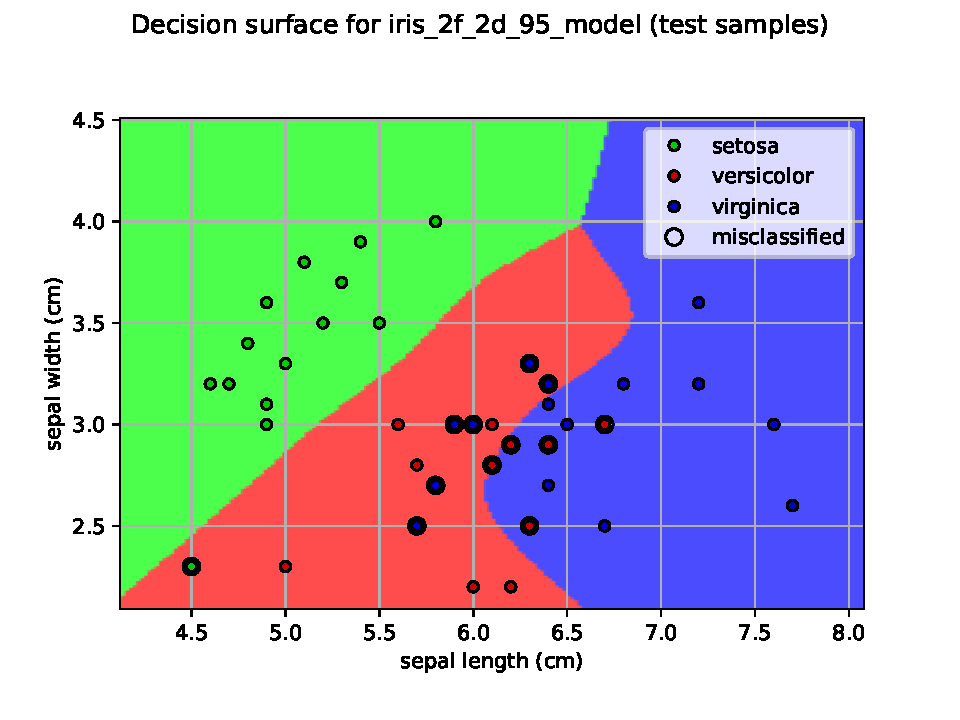
\includegraphics[width=0.49\textwidth]{figures/iris_2f_dominant_l2_surf_test.pdf}}
\subfloat[\textbf{[E8] kNN}]{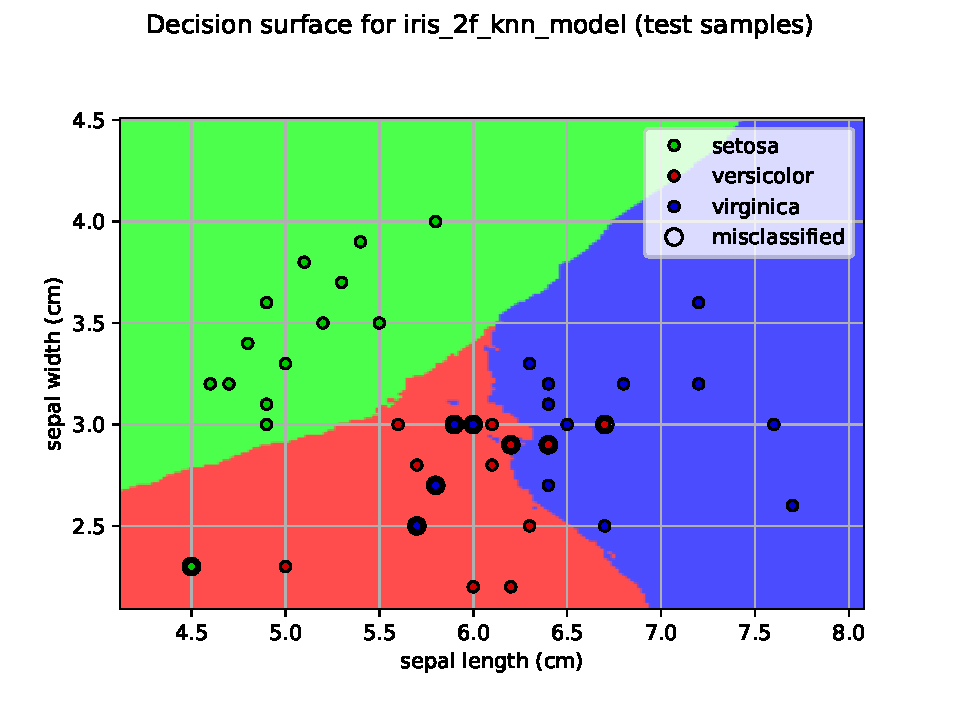
\includegraphics[width=0.49\textwidth]{figures/iris_2f_knn_surf_test.pdf}}\\
\subfloat[\textbf{[E9] XGBoost}]{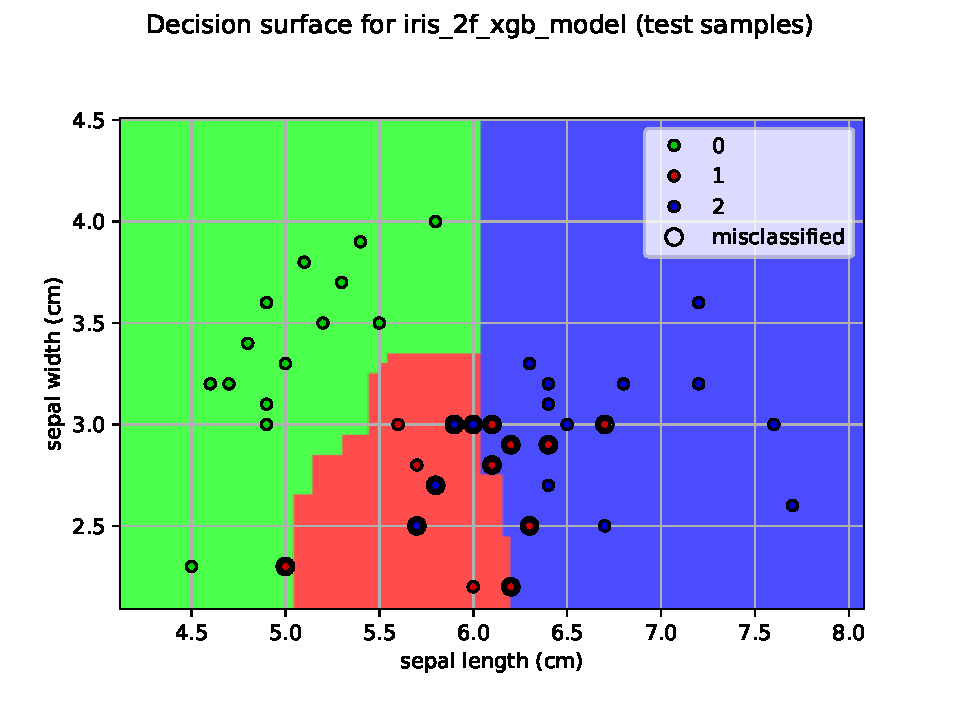
\includegraphics[width=0.49\textwidth]{figures/iris_2f_xgb_surf_test.pdf}}
\end{center}
\end{figure}
%
We draw the following conclusions from this study:
%
\begin{itemize}
\item In terms of achieving a low log-loss, proset appears to rank in-between XGBoost and kNN.
%
\item Proset achieves a greater reduction in the number of features than XGBoost with a preference for small decision trees.
While the fit strategy for XGBoost may not always select the smallest possible feature set due to feature subsampling, the difference is marked.
%
\item The extremely good performance of XGBoost on the checker data is possibly due to the fact that the approximating function is of the same class as the target.
Both are step functions with edges parallel to the main coordinate axes.
%
\item XOR 6f appears to defeat tree ensembles, which choose features one at a time based on a greedy criterion.
No matter how the first split is made, the expected number of cases per class in each resulting subspace is 50 \%, same as for the whole space.
Thus, the first split is always made in response to random fluctuations in the data.
This is also true for the checkerboard with an even number of squares per side, but the first split is almost sure to break the symmetry for this case.
In contrast, for XOR 6f, at least five splits are required to expose the underlying structure.
The partitions created by five random splits apparently do not contain sufficient information to build a meaningful decision tree.
\end{itemize}
%
Based on these observations, we define five additional test cases to further explore the differences between the three algorithms:
%
\begin{enumerate}
\item\textbf{Checker rot:} to determine how much of the good performance of XGBoost on the checker data is due to the axis-parallel steps, we rotate the checkerboard pattern by 45\textdegree.
%
\item\textbf{XOR 3f, XOR 4f, XOR 5f:} in order to find the point at which XGBoost fails on the `continuous XOR' class of problems, we generate instances with three, four, and five features.
As for XOR 6f, these each have an average of 100 samples per orthant.
%
\item\textbf{XOR 6+6f:} to understand how easy it is to confuse the kNN classifier with irrelevant data, we add six more features to the XOR 6f problem.
These are drawn from the same distribution as the first six but have no impact on the target.
\end{enumerate}
%
\begin{table}
\caption{[E10] New examples -- results for proset classifier}
\label{tab_e10}
%
\begin{center}
\small
\begin{tabular}{|lrrrrr|}
\hline
&\multicolumn{5}{c|}{\textbf{\hrulefill\ Data set \hrulefill}}\\
&\textbf{Checker rot}&\textbf{XOR 3f}&\textbf{XOR 4f}&\textbf{XOR 5f}&\textbf{XOR 6+6f}\\
\multicolumn{6}{|l|}{\textbf{Data}}\\
Classes&2&2&2&2&2\\
Features&2&3&4&5&12\\
Samples&6,400&800&1,600&3,200&6,400\\
Train samples&4,480&560&1,120&2,240&4,480\\
Test samples&1,920&240&480&960&1,920\\
\textbf{Candidates}&1,000&$\sim280$&$\sim560$&$1000$&1,000\\
\multicolumn{6}{|l|}{\textbf{Stage 1}}\\
Optimal $\lambda_v$&$3.1\times10^{-5}$&$4.5\times10^{-2}$&$1.8\times10^{-3}$&$5.5\times10^{-3}$&$2.2\times10^{-4}$\\
Selected $\lambda_v$&$2.9\times10^{-4}$&$4.2\times10^{-3}$&$1.0\times10^{-2}$&$5.5\times10^{-3}$&$1.9\times10^{-3}$\\
Optimal $\lambda_w$&$4.3\times10^{-9}$&$1.3\times10^{-8}$&$7.7\times10^{-8}$&$8.3\times10^{-8}$&$5.7\times10^{-8}$\\
Selected $\lambda_w$&$6.9\times10^{-8}$&$1.5\times10^{-6}$&$4.6\times10^{-7}$&$8.3\times10^{-8}$&$2.7\times10^{-6}$\\
Optimal log-loss&0.18&0.19&0.30&0.40&0.55\\
Threshold&0.19&0.21&0.34&0.42&0.56\\
Selected log-loss&0.19&0.20&0.32&0.40&0.56\\
\multicolumn{6}{|l|}{\textbf{Stage 2}}\\
Optimal batches&1&6&6&5&1\\
Selected batches&1&1&1&2&1\\
Optimal log-loss&0.19&0.19&0.32&0.39&0.57\\
Threshold&0.20&0.23&0.33&0.40&0.57\\
Selected log-loss&0.19&0.23&0.33&0.39&0.57\\
\multicolumn{6}{|l|}{\textbf{Final model, scores for test data}}\\
Active features&2&3&4&5&6\\
Prototypes&320&89&124&572&425\\
Log-loss&0.18&0.17&0.28&0.39&0.56\\
ROC-AUC&0.99&0.99&0.97&0.91&0.80\\
Balanced acc.&0.95&0.96&0.91&0.83&0.72\\
\hline
\end{tabular}
\end{center}
\end{table}
%
\begin{table}
\caption{[E11]  New examples -- results for $k$-nearest neighbor classifier}
\label{tab_e11}
%
\begin{center}
\small
\begin{tabular}{|lrrrrr|}
\hline
&\multicolumn{5}{c|}{\textbf{\hrulefill\ Data set \hrulefill}}\\
&\textbf{Checker rot}&\textbf{XOR 3f}&\textbf{XOR 4f}&\textbf{XOR 5f}&\textbf{XOR 6+6f}\\
\multicolumn{6}{|l|}{\textbf{Data}}\\
Classes&2&2&2&2&2\\
Features&2&3&4&5&12\\
Samples&6,400&800&1,600&3,200&6,400\\
Train samples&4,480&560&1,120&2,240&4,480\\
Test samples&1,920&240&480&960&1,920\\
\multicolumn{6}{|l|}{\textbf{Cross-validation}}\\
Optimal $k$&10&7&8&9&100\\
Selected $k$&11&16&9&13&100\\
Optimal log-loss&0.23&0.22&0.34&0.43&0.70\\
Threshold&0.24&0.27&0.35&0.44&0.71\\
Selected log-loss&0.24&0.27&0.34&0.44&0.70\\
\multicolumn{6}{|l|}{\textbf{Final model, scores for test data}}\\
Log-loss&0.21&0.25&0.31&0.45&0.71\\
ROC-AUC&0.98&0.98&0.95&0.88&0.46\\
Balanced acc.&0.92&0.91&0.86&0.80&0.48\\
\hline
\end{tabular}
\end{center}
\end{table}
%
\begin{table}
\caption{[E12]  New examples -- results for XGBoost classifier}
\label{tab_e12}
%
\begin{center}
\small
\begin{tabular}{|lrrrrr|}
\hline
&\multicolumn{5}{c|}{\textbf{\hrulefill\ Data set \hrulefill}}\\
&\textbf{Checker rot}&\textbf{XOR 3f}&\textbf{XOR 4f}&\textbf{XOR 5f}&\textbf{XOR 6+6f}\\
\multicolumn{6}{|l|}{\textbf{Data}}\\
Classes&2&2&2&2&2\\
Features&2&3&4&5&12\\
Samples&6,400&800&1,600&3,200&6,400\\
Train samples&4,480&560&1,120&2,240&4,480\\
Test samples&1,920&240&480&960&1,920\\
\multicolumn{6}{|l|}{\textbf{Stage 1}}\\
Optimal max.\ depth&21&7&18&17&1\\
Selected max.\ depth&12&6&11&12&1\\
Optimal colsample&0.77&0.81&0.79&0.72&0.81\\
Selected colsample&0.26&0.88&0.88&0.81&0.81\\
Optimal subsample&0.43&0.84&0.77&0.69&0.25\\
Selected subsample&0.54&0.81&0.88&0.49&0.25\\
Optimal log-loss&0.18&0.10&0.30&0.64&0.70\\
Threshold&0.19&0.11&0.32&0.67&0.70\\
Selected log-loss&0.19&0.11&0.31&0.66&0.70\\
\multicolumn{6}{|l|}{\textbf{Stage 2}}\\
Optimal iterations&8,455&2,677&2,926&895&2\\
Selected iterations&3,364&690&1,154&96&1\\
Optimal log-loss&0.13&0.10&0.28&0.65&0.69\\
Threshold&0.14&0.15&0.31&0.68&0.69\\
Selected log-loss&0.14&0.15&0.31&0.68&0.69\\
\multicolumn{6}{|l|}{\textbf{Final model, scores for test data}}\\
Active features&2&3&4&5&1\\
Log-loss&0.12&0.11&0.23&0.67&0.69\\
ROC-AUC&0.99&1.00&0.98&0.65&0.50\\
Balanced acc.&0.95&0.97&0.94&0.60&0.50\\
\hline
\end{tabular}
\end{center}
\end{table}
%
\begin{table}
\caption{[E10, E11, E12] Comparison of results (best log-loss bold)}
\label{tab_e10_e11_e12}
%
\begin{center}
\small
\begin{tabular}{|lrrrrr|}
\hline
&\multicolumn{5}{c|}{\textbf{\hrulefill\ Data set \hrulefill}}\\
&\textbf{Checker rot}&\textbf{XOR 3f}&\textbf{XOR 4f}&\textbf{XOR 5f}&\textbf{XOR 6+6f}\\
\multicolumn{6}{|l|}{\textbf{[E10] Proset with randomized search for $\lambda_v$ and $\lambda_w$ ($\alpha_v=\alpha_w=0.95$)}}\\
Active features&2&3&4&5&6\\
Log-loss&0.18&0.17&0.28&\textbf{0.39}&\textbf{0.56}\\
Threshold stage 2&0.20&0.23&0.33&0.40&0.57\\
ROC-AUC&0.99&0.99&0.97&0.91&0.80\\
Balanced acc.&0.95&0.96&0.91&0.83&0.72\\
\multicolumn{6}{|l|}{\textbf{[E11] $k$-nearest neighbor classifier with grid search for $k$}}\\
Active features&2&3&4&5&12\\
Log-loss&0.21&0.25&0.31&0.45&0.71\\
Threshold CV&0.24&0.27&0.35&0.44&0.71\\
ROC-AUC&0.98&0.98&0.95&0.88&0.46\\
Balanced acc.&0.92&0.91&0.86&0.80&0.48\\
\multicolumn{6}{|l|}{\textbf{[E12] XGBoost classifier with randomized parameter search}}\\
Active features&2&3&4&5&1\\
Log-loss&\textbf{0.12}&\textbf{0.11}&\textbf{0.23}&0.67&0.69\\
Threshold stage 2&0.14&0.15&0.31&0.68&0.69\\
ROC-AUC&0.99&1.00&0.98&0.65&0.50\\
Balanced acc.&0.95&0.97&0.94&0.60&0.50\\
\hline
\end{tabular}
\end{center}
\end{table}
%
\clearpage
%
Results for proset, kNN, and XGBoost are summarized in Tables \ref{tab_e10}, \ref{tab_e11}, and \ref{tab_e12}.
A comparison of the three algorithms is shown in Table \ref{tab_e10_e11_e12}:
%
\begin{enumerate}
\item\textbf{Checker rot:} XGBoost still yields the best model on this pattern, but the log-loss is higher than for the original checkerboard.
The largest value for maximum tree depth used in cross-validation was set to 29 as smaller bounds meant the bound was selected.
The metrics for the other two models are very similar to the original case.
%
\item\textbf{XOR 3f, XOR 4f, XOR 5f:} with three features, XGBoost performs better than other models, with four it is still best but the others are equivalent, and with five features, proset is better than the other two models, i.e., they are not affected by the orientation of the pattern.
%
\item\textbf{XOR 6+6f:} proset correctly selects the six relevant features and produces a model that is slightly worse than for the original XOR 6f.
Neither kNN nor XGBoost are able to find any structure and return constant estimators.
\end{enumerate}
%
Overall, we believe that these results show that proset is a worthwhile addition to the supervised learning toolbox.
As intended, it performs feature selection as an integral part of model fitting and is able to identify a nonlinear relationship between the features and target.
%
\section{Timing and larger benchmark cases}
\label{sec_timing_larger_cases}
%
\begin{center}\fbox{\parbox{0.95\textwidth}{\small
Except where noted, the results in this section were generated using version 0.2.0 of Python package \texttt{proset}.
Different versions of \texttt{proset} or the underlying compute libraries may yield results that are qualitatively similar but not identical.
}}\end{center}
%
To fit a proset classifier, we need to solve a sequence of optimization problems with several hundreds or thousands of variables.
Extending this to larger data sets than the initial benchmark cases requires efficient code to save memory and compute time.
For this purpose, version 0.2.0 of Python package \texttt{proset} implements several measures to improve performance:
%
\begin{enumerate}
\item All floating point arrays are stored with 32 bit precision and Fortran-contiguous layout instead of the \texttt{numpy} \cite{Harris_20} default of 64 bit C-contiguous arrays.
Inner products are computed using a low-level interface to the linear algebra kernel exposed through \texttt{scipy} \cite{Virtanen_20}.
%
\item The tolerance for the convergence check of the L-BFGS-B solver is no longer set to the default value but can be adjusted by the experimenter.
See below for a discussion.
%
\item Model fitting can use \texttt{tensorflow} \cite{Abadi_15} as alternative to \texttt{numpy}, which enables GPU usage.
Scoring still employs \texttt{numpy} exclusively.
The implementation based on \texttt{tensorflow} does not rely on stochastic gradient descent as is usual for deep learning but computes the objective function and gradient for an entire batch.
This permits L-BFGS-B to work in the same way as for the \texttt{numpy} version of the code.
%
\item Memory usage for scoring is reduced.
The original code creates a matrix with one row per sample to be scored and one column per prototype across all batches.
Version 0.2.0 limits the number of samples scored at a time and aggregates prototype contributions per batch.
While this requires nested for-loops, the number of iterations is small and the computational overhead negligible.
%
\item Memory usage for model fitting can be controlled by randomly splitting the training data into a number of `chunks' of equal size.
Each chunk is added as a separate batch to the model.
If the specified number of batches exceeds the number of chunks, additional random splits are generated.
\end{enumerate}
%
To check for convergence of L-BFGS-B, version 0.1.0 of \texttt{proset} uses the recommended default settings.
Processing a single batch often requires several hundred function and gradient evaluations.
If we study individual iterations, it appears that the feature weights $v_c$ converge more quickly than the prototype weights $w_{c,j}$.
In particular, if a data set admits a feature-sparse solution, the active features are found quickly.
After that point, the algorithm spends considerable time on reducing the number of prototypes, which has only a small impact on the objective function.
This is not surprising, since feature weights determine the global behavior of the model, while prototype weights only affect predictions in a neighborhood of their prototype.
Thus, we can save compute time by increasing the tolerance for convergence in terms of the objective function value.
The resulting solution can have additional prototypes over a more `accurate' one, but the increase in the loss functions is likely to be negligible.\par
%
The convergence check for L-BFGS-B is controlled by a parameter called $\text{factr}$.
Let $f_i,f_{i+1}\in\R$ be the objective function value at iterations $i$ and $i+1$ respectively, and let $\epsilon>0$ be the machine precision.
The algorithm stops at iteration $n+1$ if the following condition is satisfied:
%
\begin{equation}
\frac{|f_{i}-f_{i+1}|}{\max(|f_{i}|,|f_{i+1}|,1)}\leq\text{factr}\times\epsilon\label{eq_l_bfgs_b_stop}
\end{equation}
%
The default value is $\text{factr}=10^7$, while $\text{factr}=10^{12}$ is said to produce a solution of low accuracy.
In the following, we consider a value of $\text{factr}=10^{10}$ as an alternative to the default.
Note that L-BFGS-B also stops if the gradient has a small norm or an upper bound on the number of iterations is reached, but these criteria do not allow us to exploit the observed behavior.\par
%
Our first experiment [E13] for evaluating the changes is to repeat the model fit for the iris 2f, wine, cancer, digits, and checker data of Section \ref{sec_classifier_benchmarks} with different settings.
Model hyperparameters are those from experiment [E3], i.e., $\alpha_v=\alpha_w=0.95$ with cross-validated search for $\lambda_v$ and $\lambda_w$ in stage 1 and the number of batches in stage 2.
The goal is to show that measures 1.\ and 2.\ reduce computation time and measure 5.\ does not unduly increase it.
As the data sets are fairly small, we only include timings for \texttt{tensorflow} with GPU support for the digits and checker cases.
Likewise, training data is never broken up into chunks as memory requirements are modest.
Table \ref{tab_faster_timing} shows timing results as follows:
%
\begin{description}
\item[Data set:] the name of the benchmark data set.
%
\item[Version:] \texttt{proset} package version, either `0.1.0', `0.2.0'.
Training with tensorflow is indicated by `\texttt{tf}'.
Results for XGBoost are also shown for comparison under `\texttt{xgb}'.
While the cross-validation strategy for this algorithm is different, we consider that it expends similar effort to find suitable hyperparameters.
As a kNN classifier has totally different fit strategy -- it stores the entire training data in a format optimized for neighborhood search -- no results are shown for this algorithm.
%
\item[Precision:] 32 bit or 64 bit for float arrays.
%
\item[Tolerance:] the value of parameter $\text{factr}$.
Settings are $10^{7}$, $10^{10}$, and `mixed', which is $10^{10}$ for cross-validation and $10^{7}$ for the final model fit.
The latter is a safeguard in case increasing tolerance degrades model quality slightly but not beyond the point where cross-validation can find good hyperparameters.
%
\item[Duration, Absolute:] the time in seconds for the entire cross-validation run.
This is always the middle value from a set of three trials.
%
\item[Duration, Relative:] the time as a percentage of the duration for package version 0.1.0.
\end{description}
%
Computations using \texttt{numpy} only were made on a PC with four Intel(R) Core(TM) i5-6500 CPU @ 3.20GHz and 8 GB RAM.
The code was executed under Python 3.8 with \texttt{numpy} 1.22.3 using the OpenBLAS linear algebra package \cite{Wang_13}.
Training with \texttt{tensorflow} was tested on Kaggle notebooks\footnote{Available at \url{www.kaggle.com}.} with two Intel(R) Xeon(R) CPU @ 2.00GHz and 13 GB RAM, as well as a Tesla P100 GPU with 16 GB VRAM.
This used Python 3.7\footnote{Python package \texttt{proset} is developed and tested on Python 3.8 but can be installed and executed on Python 3.7 if disabling version and dependency checks, provided dependencies are installed separately.} with \texttt{numpy} 1.21.6 and OpenBLAS.\par
%
\begin{table}
\caption{[E13] Faster computations: timing comparison}
\label{tab_faster_timing}
%
\begin{center}
\small
\begin{tabular}{|lcccrr|}
\hline
&&&&\multicolumn{2}{c|}{\hrulefill\ \textbf{Runtime} \hrulefill}\\
\textbf{Data set}&\textbf{Version}&\textbf{Precision}&\textbf{Tolerance}&\textbf{Absolute}&\textbf{Relative}\\
\textbf{Iris 2f}&0.1.0&64 bit&$10^7$&20 s&100 \%\\
&0.2.0&32 bit&$10^7$&22 s&110 \%\\
&0.2.0&32 bit&$10^{10}$&8 s&40 \%\\
&0.2.0&32 bit&mixed&8 s&40 \%\\
&\texttt{xgb}&32 bit&n/a&32 s&160 \%\\
&&&&&\\
\textbf{Wine}&0.1.0&64 bit&$10^7$&21 s&100 \%\\
&0.2.0&32 bit&$10^7$&22 s&105 \%\\
&0.2.0&32 bit&$10^{10}$&8 s&38 \%\\
&0.2.0&32 bit&mixed&8 s&38 \%\\
&\texttt{xgb}&32 bit&n/a&32 s&152 \%\\
&&&&&\\
\textbf{Cancer}&0.1.0&64 bit&$10^7$&100 s&100 \%\\
&0.2.0&32 bit&$10^7$&88 s&88 \%\\
&0.2.0&32 bit&$10^{10}$&29 s&29 \%\\
&0.2.0&32 bit&mixed&29 s&29 \%\\
&\texttt{xgb}&32 bit&n/a&24 s&24 \%\\
&&&&&\\
\textbf{Digits}&0.1.0&64 bit&$10^7$&1,626 s&100 \%\\
&0.2.0&32 bit&$10^7$&682 s&42 \%\\
&0.2.0&32 bit&$10^{10}$&177 s&11 \%\\
&0.2.0&32 bit&mixed&200 s&12 \%\\
&0.2.0 + \texttt{tf}&32 bit&mixed&306 s&19 \%\\
&\texttt{xgb}&32 bit&n/a&281 s&17 \%\\
&&&&&\\
\textbf{Checker}&0.1.0&64 bit&$10^7$&9,151 s&100 \%\\
&0.2.0&32 bit&$10^7$&5,117 s&56 \%\\
&0.2.0&32 bit&$10^{10}$&3,899 s&43 \%\\
&0.2.0&32 bit&mixed&3,849 s&42 \%\\
&0.2.0 + \texttt{tf}&32 bit&mixed&452 s&5 \%\\
&\texttt{xgb}&32 bit&n/a&171 s&2 \%\\
\hline
\end{tabular}
\end{center}
\end{table}
%
Results in Table \ref{tab_faster_timing} show that reducing precision has a negligible effect on the two smallest cases iris 2f and wine.
In fact, computations appear to be slightly slower, possibly because the linear algebra kernel is optimized for 64 bit.
For the larger cancer, digits, and checker data sets, computation speed improves visibly.
As reducing precision also halves the memory requirement, the measure is clearly sensible.\par
%
Increasing the tolerance for the convergence check is beneficial in all cases.
As most of the compute time is spent on cross-validation, the `mixed' solutions perform equally well compared to the trials where the final model is also fitted with $\text{factr}=10^{10}$.\par
%
For the digits data, using \texttt{tensorflow} is slower than the optimized \texttt{numpy} implementation.
Apparently, GPU usage incurs an overhead that is not balanced by faster computations for the small number of samples.
This is different for the checker case, where \texttt{tensorflow} leads to a considerable improvement.
The granular structure of the checker pattern creates a difficult optimization problem for proset that requires many iterations to solve.
Conversely, as the target can be replicated exactly by a decision tree, the task is especially easy for XGBoost.\par
%
Even without GPU support, the measures are able to reduce compute time to less than half compared to version 0.1.0 in all cases.
It remains to be seen whether increasing the tolerance has a negative impact on model quality.
Table \ref{tab_faster_performance} shows the model structure and log-loss achieved for the trials.
The first five columns contain the same information as for the timing comparison, the remaining fields are:
%
\begin{description}
\item[Features:] the number of features in the final model.
%
\item[Proto.:] the number of prototypes in the final model.
%
\item[Log-loss:] the log-loss achieved by the final model.
%
\item[Threshold] the upper bound on log-loss established in the second stage of cross-validation for the `1 SE rule'.
Refer to Section \ref{sec_classifier_fit} for details.
\end{description}
%
\begin{table}
\caption{[E13] Faster computations: model performance}
\label{tab_faster_performance}
%
\begin{center}
\small
\begin{tabular}{|lcccrrrr|}
\hline
\textbf{Data set}&\textbf{Version}&\textbf{Precision}&\textbf{Tolerance}&\textbf{Features}&\textbf{Proto.}&\textbf{Log-loss}&\textbf{Threshold}\\
\textbf{Iris 2f}&0.1.0&64 bit&$10^7$&2&50&0.45&0.57\\
&0.2.0&32 bit&$10^7$&2&50&0.43&0.55\\
&0.2.0&32 bit&$10^{10}$&2&55&0.44&0.58\\
&0.2.0&32 bit&mixed&2&50&0.43&0.55\\
&\texttt{xgb}&32 bit&n/a&2&n/a&0.63&0.62\\
&&&&&&&\\
\textbf{Wine}&0.1.0&64 bit&$10^7$&7&52&0.14&0.16\\
&0.2.0&32 bit&$10^7$&8&51&0.14&0.16\\
&0.2.0&32 bit&$10^{10}$&5&46&0.19&0.17\\
&0.2.0&32 bit&mixed&5&45&0.19&0.17\\
&\texttt{xgb}&32 bit&n/a&13&n/a&0.11&0.11\\
&&&&&&&\\
\textbf{Cancer}&0.1.0&64 bit&$10^7$&4&54&0.13&0.15\\
&0.2.0&32 bit&$10^7$&4&52&0.13&0.15\\
&0.2.0&32 bit&$10^{10}$&4&84&0.13&0.15\\
&0.2.0&32 bit&mixed&4&52&0.13&0.15\\
&\texttt{xgb}&32 bit&n/a&29&n/a&0.12&0.14\\
&&&&&&&\\
\textbf{Digits}&0.1.0&64 bit&$10^7$&20&493&0.16&0.19\\
&0.2.0&32 bit&$10^7$&20&487&0.16&0.18\\
&0.2.0&32 bit&$10^{10}$&30&861&0.18&0.20\\
&0.2.0&32 bit&mixed&29&605&0.16&0.20\\
&0.2.0 + \texttt{tf}&32 bit&mixed&29&613&0.17&0.19\\
&\texttt{xgb}&32 bit&n/a&53&n/a&0.11&0.14\\
&&&&&&&\\
\textbf{Checker}&0.1.0&64 bit&$10^7$&2&328&0.18&0.20\\
&0.2.0&32 bit&$10^7$&2&316&0.18&0.20\\
&0.2.0&32 bit&$10^{10}$&2&357&0.18&0.20\\
&0.2.0&32 bit&mixed&2&316&0.18&0.20\\
&0.2.0 + \texttt{tf}&32 bit&mixed&2&315&0.18&0.20\\
&\texttt{xgb}&32 bit&n/a&2&n/a&0.06&0.09\\
\hline
\end{tabular}
\end{center}
\end{table}
%
Model performance behaves differently for each data set:
%
\begin{description}
\item[Iris 2f:] all proset models are equivalent in terms of log-loss.
The selected hyperparameters are $\lambda_v=1.1\times10^{-2}$ and $\lambda_w=1.0\times10^{-5}$ and either 2 batches (version 0.1.0 and version 0.2.0 with tolerance 10$^{10}$) or 3 batches (version 0.2.0 with tolerance 10$^7$ and mixed).
As expected, the final model fitted with increased tolerance has slightly more prototypes.
%
\item[Wine:] the wine data is the only case that shows strictly worse performance when relaxing the tolerance.
This is due to different hyperparameters getting selected.
The models fitted with $\text{factr}=10^7$ use $\lambda_v=1.1\times10^{-2}$, $\lambda_w=1.8\times10^{-5}$, and 2 batches.
Those fitted with $\text{factr}=10^{10}$ use $\lambda_v=3.5\times10^{-3}$, $\lambda_w=3.1\times10^{-5}$, and a single batch.
Note that for the latter models, the final log-loss of 0.19 is worse than the threshold of 0.17 found in stage 2.
This indicates that the small size of the data set already causes a large variance in results, so the choice of tolerance may not be at fault.
%
\item[Cancer:] all proset models are equivalent in terms of log-loss.
The hyperparameters are also the same in each case ($\lambda_v=1.1\times10^{-2}$, $\lambda_w=1.8\times10^{-5}$, 1 batch).
The only difference is that the number of prototypes is smaller if the final model is fitted with $\text{factr}=10^7$, which is exactly the expected behavior.
%
\item[Digits:] the proset models are equivalent in terms of the threshold, but final models fitted with $\text{factr}=10^7$ achieve a slightly lower log-loss.
The `mixed' approach yields the same model quality as using $\text{factr}=10^7$ throughout, although the hyperparameters are in fact different.
Cross-validation with $\text{factr}=10^7$ selects $\lambda_v=9.5\times10^{-4}$, $\lambda_w=5.6\times10^{-9}$, and 1 batch.
For $\text{factr}=10^{10}$, the values are $\lambda_v=5.5\times10^{-3}$, $\lambda_w=8.3\times10^{-8}$, and 2 batches.
%
\item[Checker:] all proset models are equivalent in terms of log-loss.
They also use the same hyperparameters $\lambda_v=2.9\times10^{-4}$, $\lambda_w=6.9\times10^{-8}$, and 1 batch.
The only difference is that fitting a final model with relaxed tolerance retains slightly more prototypes.
\end{description}
%
Based on these trials, the `mixed' approach appears to be a good strategy for saving compute time without decreasing model performance.
The software was extended accordingly: Python package \texttt{proset} specifies $\text{factr}=10^7$ as default for fitting a single model, but the convenience function for cross-validated selection of hyperparameters uses the `mixed' settings.\par
%
The second experiment [E14] for evaluating the changes uses \texttt{tensorflow} to fit models on two data sets that are considerably larger:
%
\begin{enumerate}
\item\textbf{MNIST:} greyscale images showing handwritten digits with a 28-by-28 resolution comprising
60,000 training and 10,000 test samples.
The data was collected from two different groups of people, Census Bureau employees and high-school students.
Digits from the former group (the second half of the test data) are known to be easier to classify.\par
%
The MNIST digits are well-studied case in machine-learning research.
Both the data and an extensive overview of related publications with achievable error rates is hosted online by Yann LeCun \cite{LeCun_98}.
%
\item\textbf{CIFAR-10:} RGB images of 10 classes of objects downsampled to a 32-by-32 resolution with 50,000 training and 10,000 test samples.
This is another popular test case for machine learning hosted online by Alex Krizhevsky \cite{Krizhevsky_09}.\par
%
Proset is not designed to compete with deep learning methods that handle features with low information content (e.g., pixels in images).
It may still be suitable for transfer learning, where a pre-trained deep learning model converts raw data to higher-order features as input for a task-specific classifier.
Thus, we process the CIFAR-10 data through a ResNet50 \cite{He_15} model trained on the ImageNet \cite{Russakovsky_15} data set before feeding it to proset.
This results in a feature vector of length 2,048.
\end{enumerate}
%
All models use the following hyperparameters, which reflect lessons learned from previous experiments:
%
\begin{itemize}
\item $L_2$-penalty is dominant with $\alpha_v=\alpha_w=0.95$ (cp.\ [E3]).
%
\item Vary $\lambda_v$ on a grid with 11 points logarithmically spaced between $10^{-6}$ and $10^{-1}$ but fix $\lambda_w=10^{-8}$ (cp.\ [E5]).
%
\item Draw 10,000 candidates for prototypes per batch to account for the more complex structure of the data and larger sample size.
%
\item Split the training data into two chunks of equal size to preserve GPU memory.
See below for a discussion why this is necessary.
%
\item Test adding up to 20 batches to a model.
This is done since splitting the data into chunks means each batch contains only half of the training data.
\end{itemize}
%
Regarding memory usage, the bottleneck is not caused by the greater number of features but by the number of candidates.
The largest matrices that need to fit into GPU RAM have as many elements as the number of candidates for prototypes times the number of reference points.
For example, if we have 50,000 samples and choose 10,000 candidates, the algorithm creates several matrices with $4\times10^8$ elements (1.49 GB of 32 bit floats).
By splitting the training data into two chunks of size 25,000, we reduce the matrix size to $1.5\times10^8$ (0.56 GB).\par
%
All previous benchmarks use centering and scaling of the features as the only preprocessing step.
For MNIST and CIFAR-10, we also test the impact of applying principal component analysis (PCA).
This reduces compute time through dimension reduction and can potentially lead to better solutions as individual features represent more information.
As it depends on the initial scale of the features whether they need to be normalized before applying PCA, we try both approaches.
The principal components are always normalized to unit variance as required by proset.
For dimension reduction, we retain the components with the largest eigenvalues explaining 99 \% of the variance.
%
\begin{remark}
We do not consider problem-specific enhancements like transforms for optical character recognition applied to the MNIST data.
The goal of this experiment is to determine whether the performance enhancements allow the algorithm to process problems of the given size, not to find the absolutely best models for the benchmark data.
\end{remark}
%
Table \ref{tab_e14} shows the results of six experiments in a similar format as in Section \ref{sec_classifier_benchmarks}.
Some additional information is included:
%
\begin{description}
\item[Chunks:] training data is split into this many disjoint chunks for fitting.
%
\item[Preprocessing:] either centering and scaling (S+C), PCA (features are centered but not scaled before applying PCA), or both (features are centered and scaled before applying PCA).
%
\item[Features:] for experiments using PCA, this is the dimension of the reduced input space.
%
\item[Sparseness:] the number of active features divided by the number of input features.
%
\item[Runtime:] the duration of the full cross-validation run.
This is based on a single trial and rounded to the closest 15 minutes.
\end{description}
%
\begin{table}
\caption{[E14] Larger benchmark cases (fix $\lambda_w=10^{-8}$ and $\alpha_v=\alpha_w=0.95$)}
\label{tab_e14}
%
\begin{center}
\small
\begin{tabular}{|lrrrrrr|}
\hline
&\multicolumn{6}{c|}{\textbf{\hrulefill\ Data set \hrulefill}}\\
&\textbf{MNIST}&\textbf{MNIST}&\textbf{MNIST}&\textbf{CIFAR-10}&\textbf{CIFAR-10}&\textbf{CIFAR-10}\\
\multicolumn{7}{|l|}{\textbf{Data}}\\
Classes&10&10&10&10&10&10\\
Preprocessing&C+S&PCA&both&C+S&PCA&both\\
Features&784&331&543&2,048&1,514&1,797\\
Samples&70,000&70,000&70,000&60,000&60,000&60,000\\
Train samples&60,000&60,000&60,000&50,000&50,000&50,000\\
Test samples&10,000&10,000&10,000&10,000&10,000&10,000\\
\textbf{Chunks}&2&2&2&2&2&2\\
\textbf{Candidates}&10,000&10,000&10,000&10,000&10,000&10,000\\
\multicolumn{7}{|l|}{\textbf{Stage 1}}\\
Optimal $\lambda_v$&$3.2\times10^{-6}$&$1.0\times10^{-4}$&$1.0\times10^{-6}$&$1.0\times10^{-3}$&$1.0\times10^{-2}$&$3.2\times10^{-4}$\\
Selected $\lambda_v$&$1.0\times10^{-2}$&$3.2\times10^{-3}$&$3.2\times10^{-3}$&$3.2\times10^{-3}$&$1.0\times10^{-2}$&$1.0\times10^{-2}$\\
Optimal log-loss&0.38&0.27&0.39&1.33&1.41&1.45\\
Threshold&0.39&0.28&0.40&1.34&1.42&1.47\\
Selected log-loss&0.39&0.28&0.39&1.33&1.41&1.46\\
\multicolumn{7}{|l|}{\textbf{Stage 2}}\\
Optimal batches&3&2&5&8&4&2\\
Selected batches&3&2&3&5&2&2\\
Optimal log-loss&0.33&0.26&0.38&1.27&1.38&1.43\\
Threshold&0.34&0.26&0.39&1.28&1.39&1.44\\
Selected log-loss&0.33&0.26&0.38&1.28&1.39&1.43\\
\multicolumn{7}{|l|}{\textbf{Final model, scores for test data}}\\
Active features&104&25&16&195&18&14\\
Sparseness&0.13&0.08&0.03&0.10&0.01&0.01\\
Prototypes&12,877&12,198&5,553&23,290&7,881&6,925\\
Log-loss&0.31&0.23&0.33&1.25&1.36&1.38\\
ROC-AUC&1.00&1.00&0.99&0.91&0.90&0.89\\
Balanced acc.&0.94&0.95&0.91&0.56&0.52&0.52\\
\textbf{Runtime}&4:00 h&2:30 h&3:00 h&3:00 h&2:45 h&3:30 h\\
\hline
\end{tabular}
\end{center}
\end{table}
%
For all trials, selected values for $\lambda_v$ are similar to those for the smaller benchmark cases and close to the value $10^{-3}$ chosen as default.
Testing up to 20 batches during cross-validations turns out to be unnecessary as both the optimal and selected number stay below 10.
Based on the previous observation regarding the number of candidates, it would probably be better to fit a larger first batch with more candidates, but this is not possible given available GPU RAM.
Apart from these observations, there are considerable differences between the data sets:
%
\begin{enumerate}
\item\textbf{MNIST:} if we use the threshold on log-loss from the second stage to determine whether models are equivalent, the model fitted after applying PCA to unscaled features strictly outperforms the other two.
PCA for scaled features performs worst although the resulting log-loss is still equivalent to the model that uses only centering and scaling.
As the greyscale values already have a common scale, converting them to unit variance before PCA apparently degrades performance by magnifying pixel noise.\par
%
The balanced accuracy of 95 \% is comparable to the 5 \% error rate on the test set reported in \cite{LeCun_98} for the kNN algorithm with Euclidean distance.
Note that the latter score does not balance the classes, but the test set is close enough to being balanced so the difference is negligible.
Considerable better performance up to 0.7 \% test error rate is reported in the cited publication for convolutional neural networks (CNN).
An even lower test error rate of 0.23 \% is reported in \cite{Ciresan_12} also for CNNs.
%
\item\textbf{CIFAR-10:} using only centering and scaling for the features strictly outperforms PCA.
This may be because the features have lower bound of zero, which indicates the effective absence of a particular property.
The linear combination of multiple features generated by PCA can obscure this information.\par
%
The best proset model is still not very good with a balanced accuracy of 56 \%.
The technical report \cite{Krizhevsky_09} introducing the CIFAR-10 data shows around 60 \% test accuracy for logistic regression applied to features generated from a RBM (Restricted Boltzmann Machine) model.
A CNN using the ResNet50 architecture can achieve test error rates below 7 \% \cite{He_15}.
\end{enumerate}
%
In conclusion, [E14] shows that the performance enhancements allow us to fit proset models to larger data sets.
However, we find no particular aptitude for handling what is commonly called `unstructured data' even after preprocessing to obtain more informative features.
%
\begin{center}\fbox{\parbox{0.95\textwidth}{\small
Version 0.3.0 of Python package \texttt{proset} replaced the chunking mechanism with the option to set an upper bound on the number of samples per batch.
The reasons for this change and updated benchmark results are given below.
}}\end{center}
%
While studying classification problems outside the scope of the benchmark study, we found that splitting the data into disjoint chunks of equal size is not a good approach for reducing GPU memory requirements.
The major drawback is that it limits potential batch sizes to a particular set of numbers.
This is unfortunate, as the first batch dominates the performance of the algorithm even if subsequent batches use new data.
Thus, the best approach is to choose batch size as large as possible under memory constraints.
Also, hyperparameters are selected for a specific batch size, which may not be achievable on an extended set of training data.
For these reasons, \texttt{proset} version 0.3.0 implements a different strategy for controlling GPU memory.
It allows the user to specify an upper bound on the number of samples per batch that is enforced via stratified subsampling.\par
%
\begin{table}
\caption{[E15] Larger benchmark cases with sample limit}
\label{tab_e15}
%
\begin{center}
\small
\begin{tabular}{|lrr|}
\hline
&\multicolumn{2}{c|}{\textbf{\hrulefill\ Data set \hrulefill}}\\
&\textbf{MNIST}&\textbf{CIFAR-10}\\
\multicolumn{3}{|l|}{\textbf{Data}}\\
Classes&10&10\\
Preprocessing&PCA&C+S\\
Features&331&2,048\\
Samples&70,000&60,000\\
Train samples&60,000&50,000\\
Test samples&10,000&10,000\\
\textbf{Samples per batch}&40,000&35,000\\
\textbf{Candidates}&10,000&10,000\\
\multicolumn{3}{|l|}{\textbf{Stage 1}}\\
Optimal $\lambda_v$&$3.2\times10^{-3}$&$3.2\times10^{-3}$\\
Selected $\lambda_v$&$1.0\times10^{-2}$&$1.0\times10^{-2}$\\
Optimal log-loss&0.27&1.35\\
Threshold&0.28&1.36\\
Selected log-loss&0.28&1.36\\
\multicolumn{3}{|l|}{\textbf{Stage 2}}\\
Optimal batches&1&4\\
Selected batches&1&2\\
Optimal log-loss&0.28&1.34\\
Threshold&0.29&1.34\\
Selected log-loss&0.28&1.34\\
\multicolumn{3}{|l|}{\textbf{Final model, scores for test data}}\\
Active features&16&100\\
Sparseness&0.05&0.05\\
Prototypes&8,029&13,411\\
Log-loss&0.25&1.32\\
ROC-AUC&1.00&0.91\\
Balanced acc.&0.95&0.55\\
\textbf{Runtime}&2:30 h&4:00 h\\
\hline
\end{tabular}
\end{center}
\end{table}
%
Table \ref{tab_e15} shows results for the MNIST and CIFAR-10 data using the best preprocessing methods from [E14].
For MNIST, instead of fitting two chunks with 30,000 samples each, the new results use an upper limit of 40,000 samples per batch.
For CIFAR-10, chunks of 25,000 samples are replaced by batches of size 35,000.
These numbers approximate the limits of GPU memory, i.e., adding 5,000 more samples causes an out-of-memory error in each case.\par
%
The new models use fewer batches than the previous ones, so it looks like the algorithm can extract more information from larger batches.
However, overall performance is slightly worse, although results for MNIST are still equivalent in terms of the stage 2 threshold for log-loss.
For the two examples, the achieved increase in batch size appears to be too small to yield a significant improvement.
We still believe that the new approach is the better one in general.
%
\section{Updated fit strategy}
\label{sec_updated_fit}
%
\begin{center}\fbox{\parbox{0.95\textwidth}{\small
Except where noted, the results in this section were generated using version 0.4.0 of Python package \texttt{proset}.
Different versions of \texttt{proset} or the underlying compute libraries may yield results that are qualitatively similar but not identical.
}}\end{center}
%
When applying the proset classifier to problems outside the scope of this report, we found that the fit strategy proposed in Section \ref{sec_classifier_fit} is not ideal.
As the penalty weights are selected for models with a single batch only, adding multiple batches can result in a modest degree of overfitting.
In turn, cross-validation tends to choose a model with a single batch, which does not always make good use of the data.
This is especially obvious if the number of samples evaluated per batch is limited due to memory constraints.
In this case, any data not included in the first batch has no impact on the model at all.
Thus, we modify the fit strategy to choose $\lambda_v$ and the number of batches in a single cross-validation step.
All other model parameters are set to the defaults established earlier.
The new approach is conceptually simpler, although it requires more computational effort than the previous strategy.
As the log-loss for most benchmark cases is reduced, we consider this an acceptable trade-off.\par
%
\begin{algorithm}[Hyperparameter selection, updated]~
\label{alg_hyperparameters_updated}
%
\begin{enumerate}
\item Fix $M$, $\eta$, $\alpha_v$, $\alpha_w$, and $\lambda_w$.
Choose a grid for $\lambda_v$ and an upper bound $B_U$ for $B$.
%
\item Split the data into a training set (70 \%) and test set (30 \%), stratified by class.
%
\item\textbf{Cross-validation}
%
\begin{enumerate}
\item Perform five-fold cross-validation on the training set for each value of $\lambda_v$ and $B_U$ batches.
%
\item Compute the mean and standard deviation of log-loss for each value of $\lambda_v$ using $0\leq B\leq B_U$ batches from the fitted models.
%
\item Determine a threshold for model quality by taking the lowest achieved mean log-loss and adding the corresponding standard deviation.
%
\item Among all combinations whose mean log-loss is less than or equal to the threshold, choose the one with the largest $\lambda_v$.
In case of multiple candidates, take the one with the smallest number of batches.
\end{enumerate}
%
\item Refit the model with the selected parameters.
%
\item Score the final model on the test data.
\end{enumerate}
\end{algorithm}
%
Python package \texttt{proset} uses default parameters $M=1,000$, $\eta=0.5$, $\alpha_v=\alpha_w=0.95$ and $\lambda_w=10^{-8}$.
The grid for $\lambda_v$ has 11 logarithmically spaced values from $10^{-6}$ to $10^{-1}$, $B_U$ is set to 10.
These settings apply to all experiments except where noted.\par
%
\begin{table}
\caption{[E16] Updated fit strategy for original benchmark cases}
\label{tab_e16}
%
\begin{center}
\small
\begin{tabular}{|lrrrrrr|}
\hline
&\multicolumn{6}{c|}{\textbf{\hrulefill\ Data set \hrulefill}}\\
&\textbf{Iris 2f}&\textbf{Wine}&\textbf{Cancer}&\textbf{Digits}&\textbf{Checker}&\textbf{XOR 6f}\\
\multicolumn{7}{|l|}{\textbf{Data}}\\
Classes&3&3&2&10&2&2\\
Features&2&13&30&64&2&6\\
Samples&150&178&569&1,797&6,400&6,400\\
Train samples&105&124&398&1,257&4,480&4,480\\
Test samples&45&54&171&540&1,920&1,920\\
\textbf{Candidates}&$\sim50$&$\sim60$&$\sim200$&$\sim630$&1,000&1,000\\
\multicolumn{7}{|l|}{\textbf{Cross-validation}}\\
Optimal $\lambda_v$&$3.2\times10^{-5}$&$3.2\times10^{-4}$&$3.2\times10^{-3}$&$3.2\times10^{-4}$&$3.2\times10^{-5}$&$1.0\times10^{-3}$\\
Selected $\lambda_v$&$1.0\times10^{-2}$&$3.2\times10^{-4}$&$3.2\times10^{-2}$&$3.2\times10^{-3}$&$1.0\times10^{-4}$&$3.2\times10^{-3}$\\
Optimal batches&1&4&6&24&6&33\\
Selected batches&1&2&1&3&2&2\\
Optimal log-loss&0.48&0.06&0.09&0.14&0.16&0.50\\
Threshold&0.67&0.09&0.13&0.17&0.17&0.52\\
Selected log-loss&0.55&0.07&0.10&0.17&0.17&0.52\\
\multicolumn{7}{|l|}{\textbf{Final model, scores for test data}}\\
Active features&2&5&3&34&2&6\\
Prototypes&17&95&39&877&525&543\\
Log-loss&0.61&0.19&0.12&0.13&0.17&0.50\\
ROC-AUC&0.83&0.99&0.99&1.00&0.99&0.83\\
Balanced acc.&0.69&0.95&0.97&0.98&0.94&0.74\\
\hline
\end{tabular}
\end{center}
\end{table}
%
\begin{table}
\caption{[E16, E3, E8, E9] Comparison of results (best log-loss bold)}
\label{tab_e16_e3_e8, e9}
%
\begin{center}
\small
\begin{tabular}{|lrrrrrr|}
\hline
&\multicolumn{6}{c|}{\textbf{\hrulefill\ Data set \hrulefill}}\\
&\textbf{Iris 2f}&\textbf{Wine}&\textbf{Cancer}&\textbf{Digits}&\textbf{Checker}&\textbf{XOR 6f}\\
\multicolumn{7}{|l|}{\textbf{[E16] Updated fit strategy for original benchmark cases}}\\
Active features&2&5&3&34&2&6\\
Log-loss&0.61&0.19&\textbf{0.12}&0.13&0.17&\textbf{0.50}\\
Threshold&0.67&0.09&0.13&0.17&0.17&0.52\\
ROC-AUC&0.83&0.99&0.99&1.00&0.99&0.83\\
Balanced acc.&0.69&0.95&0.97&0.98&0.94&0.74\\
\multicolumn{7}{|l|}{\textbf{[E3] Proset with randomized search for $\lambda_v$ and $\lambda_w$ ($\alpha_v=\alpha_w=0.95$)}}\\
Active features&2&7&4&30&2&6\\
Log-loss&\textbf{0.43}&0.14&0.13&0.15&0.18&0.52\\
Threshold stage 2&0.57&0.17&0.14&0.17&0.20&0.53\\
ROC-AUC&0.91&1.00&0.99&1.00&0.99&0.82\\
Balanced acc.&0.71&0.98&0.98&0.97&0.95&0.72\\
\multicolumn{7}{|l|}{\textbf{[E8] $k$-nearest neighbor classifier with grid search for $k$}}\\
Active features&2&13&30&64&2&6\\
Log-loss&0.48&\textbf{0.11}&0.14&0.22&0.21&0.54\\
Threshold CV&0.54&0.15&0.17&0.27&0.24&0.56\\
ROC-AUC&0.93&1.00&1.00&1.00&0.98&0.83\\
Balanced acc.&0.82&0.97&0.95&0.93&0.92&0.73\\
\multicolumn{7}{|l|}{\textbf{[E9] XGBoost classifier with randomized parameter search}}\\
Active features&2&13&29&53&2&1\\
Log-loss&0.63&\textbf{0.11}&\textbf{0.12}&\textbf{0.11}&\textbf{0.06}&0.69\\
Threshold stage 2&0.62&0.11&0.14&0.14&0.09&0.69\\
ROC-AUC&0.89&1.00&0.99&1.00&1.00&0.50\\
Balanced acc.&0.69&0.97&0.96&0.98&0.98&0.50\\
\hline
\end{tabular}
\end{center}
\end{table}
%
Table \ref{tab_e16} shows the results of applying the new fit strategy to the six original benchmark cases and Table \ref{tab_e16_e3_e8, e9} compares them to previous results for proset, kNN, and XGBoost.
Results for the Iris 2f and Wine data sets are worse than before.
For the Wine data, the log-loss for the final model is considerably larger than the threshold established during cross-validation.
This is likely due to the small amount of data, which leads to high variance when subsampling for cross-validation and candidate selection.
The four larger data sets all show an improvement.
The log-loss for the Cancer data is now the same as for XGBoost and the new solution for Checker data is strictly better than the previous one under the threshold criterion.
Note that the maximum number of batches $B_U$ was increased for the digits and XOR 6f data to obtain a solution where the minimal log-loss is not attained at the bound.\par
%
\begin{table}
\caption{[E17] Updated fit strategy for additional benchmark cases}
\label{tab_e17}
%
\begin{center}
\small
\begin{tabular}{|lrrrrr|}
\hline
&\multicolumn{5}{c|}{\textbf{\hrulefill\ Data set \hrulefill}}\\
&\textbf{Checker rot}&\textbf{XOR 3f}&\textbf{XOR 4f}&\textbf{XOR 5f}&\textbf{XOR 6+6f}\\
\multicolumn{6}{|l|}{\textbf{Data}}\\
Classes&2&2&2&2&2\\
Features&2&3&4&5&12\\
Samples&6,400&800&1,600&3,200&6,400\\
Train samples&4,480&560&1,120&2,240&4,480\\
Test samples&1,920&240&480&960&1,920\\
\textbf{Candidates}&1,000&$\sim280$&$\sim560$&$1000$&1,000\\
\multicolumn{6}{|l|}{\textbf{Cross-validation}}\\
Optimal $\lambda_v$&$3.2\times10^{-5}$&$1.0\times10^{-2}$&$1.0\times10^{-4}$&$3.2\times10^{-3}$&$3.2\times10^{-4}$\\
Selected $\lambda_v$&$1.0\times10^{-4}$&$1.0\times10^{-2}$&$1.0\times10^{-2}$&$3.2\times10^{-3}$&$1.0\times10^{-3}$\\
Optimal batches&7&1&6&9&1\\
Selected batches&6&1&1&2&1\\
Optimal log-loss&0.16&0.17&0.28&0.39&0.54\\
Threshold&0.17&0.21&0.29&0.41&0.56\\
Selected log-loss&0.17&0.17&0.29&0.40&0.55\\
\multicolumn{6}{|l|}{\textbf{Final model, scores for test data}}\\
Active features&2&3&4&5&6\\
Prototypes&551&75&165&706&551\\
Log-loss&0.16&0.18&0.28&0.38&0.53\\
ROC-AUC&0.99&0.98&0.96&0.91&0.80\\
Balanced acc.&0.95&0.93&0.87&0.81&0.72\\
\hline
\end{tabular}
\end{center}
\end{table}
%
\begin{table}
\caption{[E17, E10, E11, E12] Comparison of results (best log-loss bold)}
\label{tab_e17_e10_e11_e12}
%
\begin{center}
\small
\begin{tabular}{|lrrrrr|}
\hline
&\multicolumn{5}{c|}{\textbf{\hrulefill\ Data set \hrulefill}}\\
&\textbf{Checker rot}&\textbf{XOR 3f}&\textbf{XOR 4f}&\textbf{XOR 5f}&\textbf{XOR 6+6f}\\
\multicolumn{6}{|l|}{\textbf{[E17] Updated fit strategy for additional benchmark cases}}\\
Active features&2&3&4&5&6\\
Log-loss&0.16&0.18&0.28&\textbf{0.38}&\textbf{0.53}\\
Threshold&0.17&0.21&0.29&0.41&0.56\\
ROC-AUC&0.99&0.98&0.96&0.91&0.80\\
Balanced acc.&0.95&0.93&0.87&0.81&0.72\\
\multicolumn{6}{|l|}{\textbf{[E10] Proset with randomized search for $\lambda_v$ and $\lambda_w$ ($\alpha_v=\alpha_w=0.95$)}}\\
Active features&2&3&4&5&6\\
Log-loss&0.18&0.17&0.28&0.39&0.56\\
Threshold stage 2&0.20&0.23&0.33&0.40&0.57\\
ROC-AUC&0.99&0.99&0.97&0.91&0.80\\
Balanced acc.&0.95&0.96&0.91&0.83&0.72\\
\multicolumn{6}{|l|}{\textbf{[E11] $k$-nearest neighbor classifier with grid search for $k$}}\\
Active features&2&3&4&5&12\\
Log-loss&0.21&0.25&0.31&0.45&0.71\\
Threshold CV&0.24&0.27&0.35&0.44&0.71\\
ROC-AUC&0.98&0.98&0.95&0.88&0.46\\
Balanced acc.&0.92&0.91&0.86&0.80&0.48\\
\multicolumn{6}{|l|}{\textbf{[E12] XGBoost classifier with randomized parameter search}}\\
Active features&2&3&4&5&1\\
Log-loss&\textbf{0.12}&\textbf{0.11}&\textbf{0.23}&0.67&0.69\\
Threshold stage 2&0.14&0.15&0.31&0.68&0.69\\
ROC-AUC&0.99&1.00&0.98&0.65&0.50\\
Balanced acc.&0.95&0.97&0.94&0.60&0.50\\
\hline
\end{tabular}
\end{center}
\end{table}
%
Results for the second set of benchmark cases are shown in Tables \ref{tab_e17} and \ref{tab_e17_e10_e11_e12}.
As for the Checker data, the result for the rotated Checker data is strictly better than before.
For the XOR cases, all four solutions are equivalent to the old proset models with two having slightly better and one having slightly worse log-loss.\par
%
\begin{table}
\caption{[E18] Updated fit strategy for larger benchmark cases}
\label{tab_e18}
%
\begin{center}
\small
\begin{tabular}{|lrr|}
\hline
&\multicolumn{2}{c|}{\textbf{\hrulefill\ Data set \hrulefill}}\\
&\textbf{MNIST}&\textbf{CIFAR-10}\\
\multicolumn{3}{|l|}{\textbf{Data}}\\
Classes&10&10\\
Preprocessing&PCA&C+S\\
Features&331&2,048\\
Samples&70,000&60,000\\
Train samples&60,000&50,000\\
Test samples&10,000&10,000\\
\textbf{Samples per batch}&40,000&35,000\\
\textbf{Candidates}&10,000&10,000\\
\multicolumn{3}{|l|}{\textbf{Cross-validation}}\\
Optimal $\lambda_v$&$1.0\times10^{-3}$&$1.0\times10^{-2}$\\
Selected $\lambda_v$&$1.0\times10^{-3}$&$1.0\times10^{-2}$\\
Optimal batches&4&7\\
Selected batches&2&3\\
Optimal log-loss&0.25&1.32\\
Threshold&0.26&1.33\\
Selected log-loss&0.25&1.32\\
\multicolumn{3}{|l|}{\textbf{Final model, scores for test data}}\\
Active features&30&136\\
Sparseness&0.09&0.07\\
Prototypes&15,359&17,689\\
Log-loss&0.25&1.31\\
ROC-AUC&1.00&0.91\\
Balanced acc.&0.95&0.56\\
\textbf{Runtime}&9:00 h&7:30 h\\
\hline
\end{tabular}
\end{center}
\end{table}
%
\begin{table}
\caption{[E18, E15] Comparison of results (best log-loss bold)}
\label{tab_e18_e15}
%
\begin{center}
\small
\begin{tabular}{|lrr|}
\hline
&\multicolumn{2}{c|}{\textbf{\hrulefill\ Data set \hrulefill}}\\
&\textbf{MNIST}&\textbf{CIFAR-10}\\
\multicolumn{3}{|l|}{\textbf{[E18] Updated fit strategy for larger benchmark cases}}\\
Selected batches&2&3\\
Active features&30&136\\
Log-loss&\textbf{0.25}&\textbf{1.31}\\
Threshold&0.26&1.33\\
ROC-AUC&1.00&0.91\\
Balanced acc.&0.95&0.56\\
Runtime&9:00 h&7:30 h\\
\multicolumn{3}{|l|}{\textbf{[E15] Larger benchmark cases with sample limit}}\\
Selected batches&1&2\\
Active features&16&100\\
Log-loss&\textbf{0.25}&1.32\\
Threshold&0.28&1.34\\
ROC-AUC&1.00&0.91\\
Balanced acc.&0.95&0.55\\
Runtime&2:30 h&4:00 h\\
\hline
\end{tabular}
\end{center}
\end{table}
%
The fit strategy for [E1] to [E3] tests 50 random parameter combinations with a single batch in stage 1 and one model with 10 batches in stage 2.
The new strategy tests 11 values for $\lambda_v$ up to 10 batches each.
As the total number of batches fitted is around twice as large, the computation time is approximately doubled.
For the larger benchmark cases, the old fit strategy fixes $\lambda_w$ and performs a line search for $\lambda_v$ using the same grid proposed for the new strategy.
This means that the computation time would increase by a factor of almost 10, which is unattractive.
For this reasons, the results in Table \ref{tab_e18} were generated using smaller grids with 3 logarithmically spaced points between $1.0\times10^{-4}$ and $1.0\times10^{-2}$ for MNIST and between $1.0\times10^{-3}$ and $1.0\times10^{-1}$ for CIFAR-10.
A comparison with previous results is shown in Table \ref{tab_e18_e15}.
Both models use an extra batch and more features under the new strategy.
The metrics for the MNIST data are the same as before, log-loss for CIFAR-10 is marginally better but still equivalent in terms of the threshold.
\endinput

\chapter{Prototype set regressor}
\label{ch_regressors}
%
The regression model will be implemented in a later release of the software.
\endinput

\chapter{Explainability}
\label{ch_explainability}
%
\begin{center}\fbox{\parbox{0.95\textwidth}{\small
The results in this section were generated using various versions of Python package \texttt{proset}.
The latest version may yield different albeit qualitatively similar output.
}}\end{center}
%
During evaluation of the benchmark study, we found that proset models are very open to inspection after fitting.
This is due to their built-in feature selection and geometric structure.
In this chapter, we review diagnostic plots and other techniques that provide a better understanding of model behavior.
%
\section{Low-dimensional representations of the data}
\label{sec_low_dimensional}
%
Verification of the model structure is greatly simplified if the algorithm is able to reduce the inputs to a small set.
We can then conduct what amounts to post-fit exploratory data analysis.\par
%
In the benchmark study, the proset classifier achieves the largest reduction in the number of features for the cancer data set, where only 4 out of 30 features yield a model that is still equivalent to XGBoost in terms of log-loss (see Table \ref{tab_e3_e8_e9}).
With only four inputs, we can visually inspect all scatter plots involving a combination of two features.
Figure \ref{fig_scatter_plots_cancer} shows the positions of the prototypes (large circles) and test samples (small circles).
The three misclassified cases are circled in black.
The density plots on the diagonal show the marginal distributions for each feature, both for the prototypes (solid curves / vertical lines) and test samples (dashed curves / dots).
Two interesting findings are that (a) any pair of features allows us to distinguish the two classes fairly well and (b) the prototypes are more clearly separated with lower variance than the whole population.\par
%
\begin{figure}
\caption{Scatter plots for active features of the cancer data model}
\label{fig_scatter_plots_cancer}
%
\begin{center}
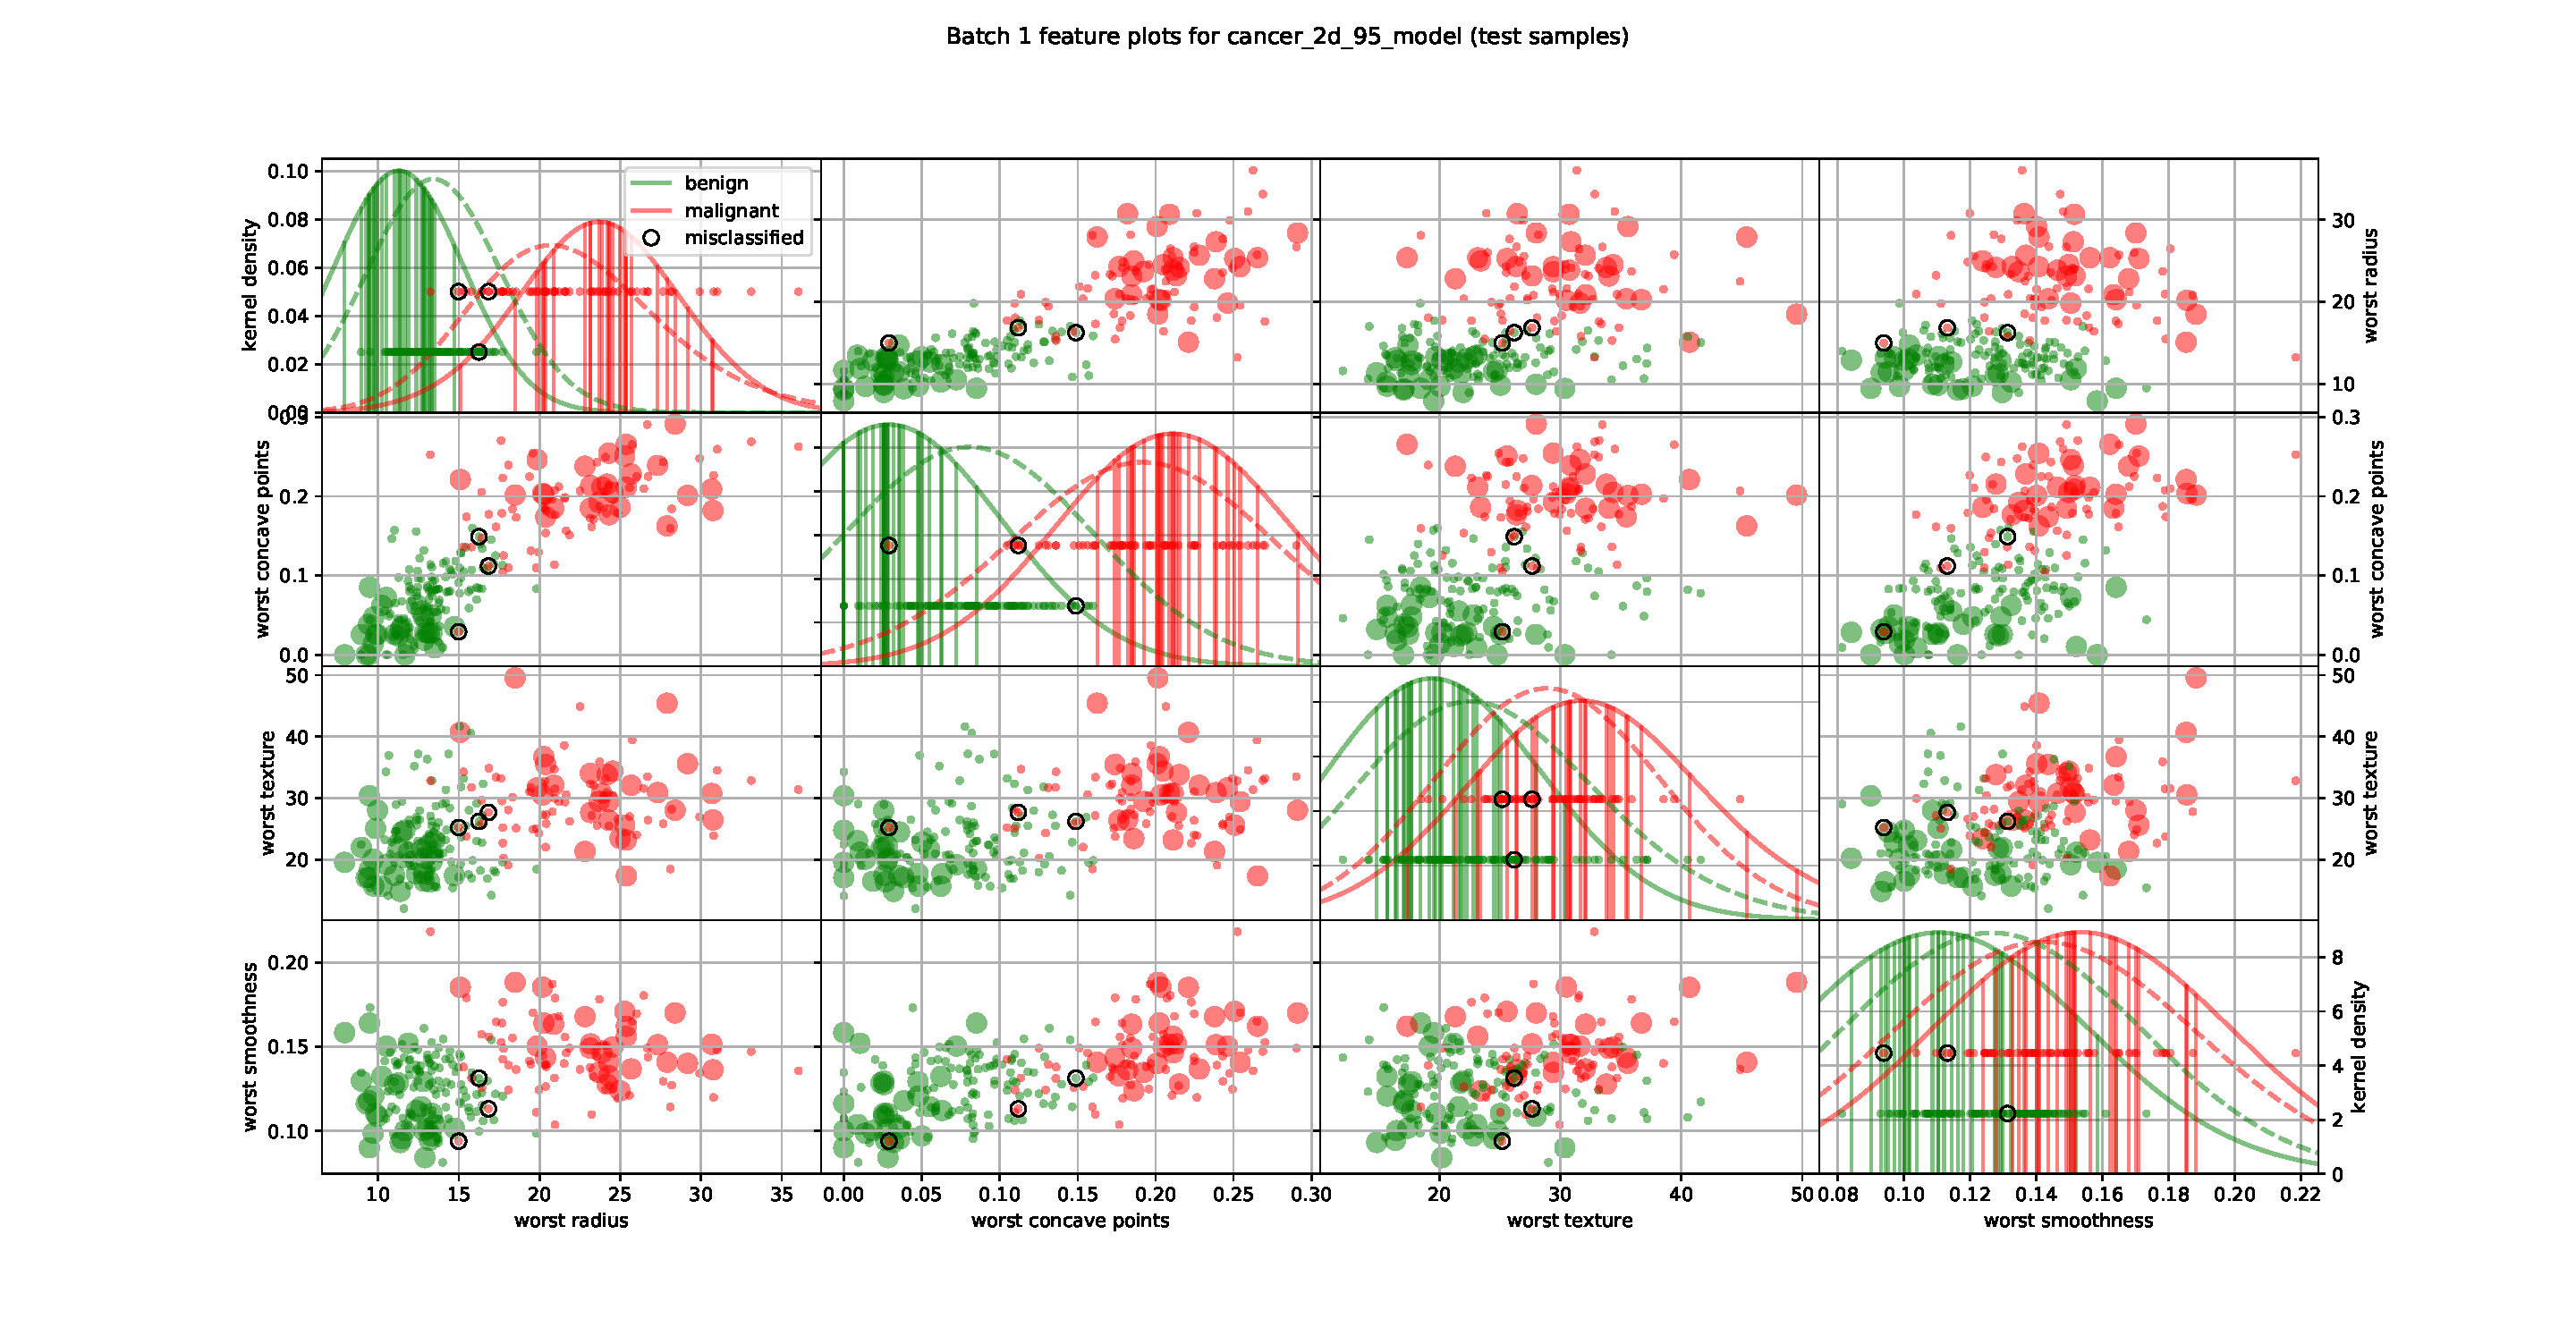
\includegraphics[width=0.9\textheight, angle=90, trim={1.5cm 1.5cm 1.5cm 0.5cm}, clip]{figures/cancer_scatter_plot_testing_data.pdf}
\end{center}
\end{figure}
%
A `small' model is also easier to review for domain experts.
For example, an oncologist should be able to provide a clear assessment whether the four features (in decreasing order of weights: worst radius, worst concave points, worst texture, worst smoothness) are a natural and sufficient choice of indicators.
If we have access to the original image data, we can ask experts to review the misclassified cases in detail and compare them to the most similar prototypes.
This can reveal labeling errors, important features excluded by the algorithm due to dearth of relevant training samples, or genuine `hard cases' that are difficult to classify even for humans.\par
%
A technique that can work even if the number of features remains large is to create low-dimensional maps of the data that take model fit results into account.
For the visualization we call the `batch 1 map', we perform doubly weighted PCA on the prototypes of the first batch:\par
%
Let $Z\in\R^{J_1\times D}$ be the matrix obtained by rescaling the features for the prototypes of the first batch with the corresponding feature weights:
%
\begin{equation}
Z_{j,d}:=v_{1,d}x_{s_{1,j},d}\label{eq_scaled_x}
\end{equation}
%
This gives larger impact to features for which the algorithm is more sensitive and removes any deselected features from the analysis.
Now let $\overline{z}$ be the row mean of $Z$ weighted using the prototype weights:
%
\begin{equation}
\overline{z}:=\frac{\sum_{j=1}^{J_1}w_{1,j}Z_{j,\bullet}}
{\sum_{j=1}^{J_1}w_{1,j}}\label{eq_weighted_mean}
\end{equation}
%
Denote by $\overline{Z}$ the centered matrix
%
\begin{equation}
\overline{Z}_{j,d}:=Z_{j,d}-\overline{z}_d\label{eq_centered_Z}
\end{equation}
%
Let $W\in\R^{J_1\times J_1}$ be the diagonal matrix with diagonal elements $w_{1,j}$ and compute the matrix decomposition
%
\begin{equation}
\overline{Z}^TW\overline{Z}=:U\Sigma U^T\label{eq_weighted_svd}
\end{equation}
%
In the above, $\Sigma$ is the diagonal matrix of eigenvalues with row and column dimension equal to the rank of $\overline{Z}^TW\overline{Z}$, while $U$ is the corresponding orthogonal matrix of eigenvectors.
If $\Sigma$ has at least rank two, the `batch 1 map' coordinates for the prototypes of the first batch are the first two columns of the product $\overline{Z}U$.
Other samples can be mapped via the same transform, i.e., scale with $v_1$, center with $\overline{z}$, and multiply with $U$.\par
%
\begin{figure}
\caption{`Batch 1 map' of cancer data showing test samples}
\label{fig_batch_1_map_test}
%
\begin{center}
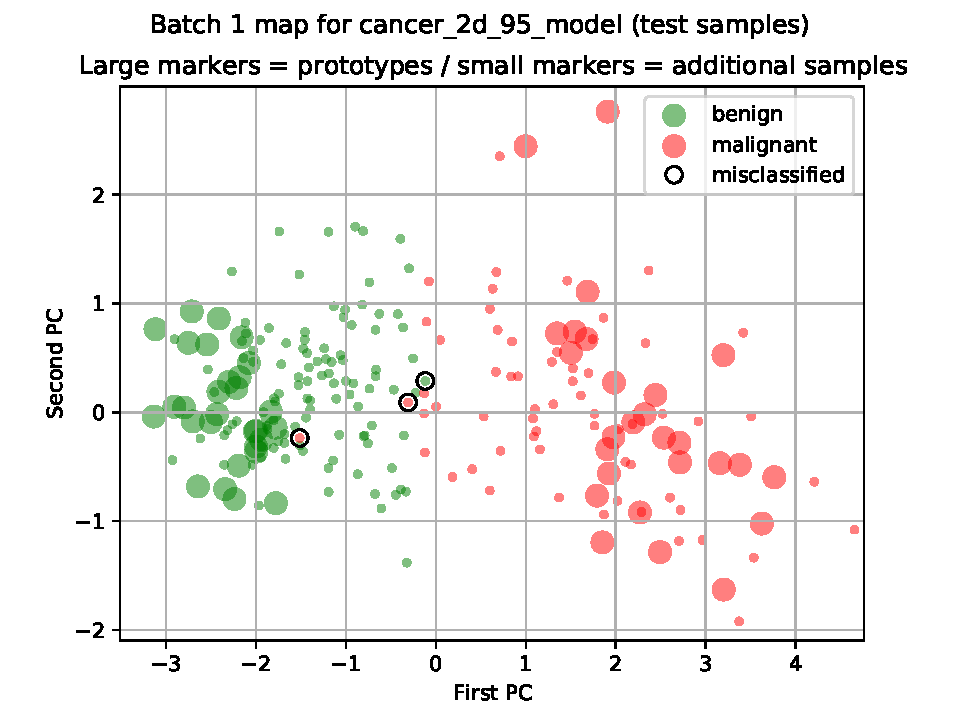
\includegraphics[height=0.4\textheight]{figures/cancer_batch_1_map_testing_data.pdf}
\end{center}
\end{figure}
%
The `batch 1 map' for the prototypes and test set of the cancer data is shown in Figure \ref{fig_batch_1_map_test}.
It appears that the two classes are almost linearly separable except for the three misclassified samples.
Two are close to the boundary between the classes, while the last is a `malignant' case surrounded by `benign' cases.
%
\section{Assessing the familiarity of new samples}
\label{sec_familiarity}
%
\begin{figure}
\caption{Model behavior outside the `area of competence'}
\label{fig_area_of_competence}
%
\begin{center}
\subfloat[\textbf{kNN on the rotated checkerboard}]{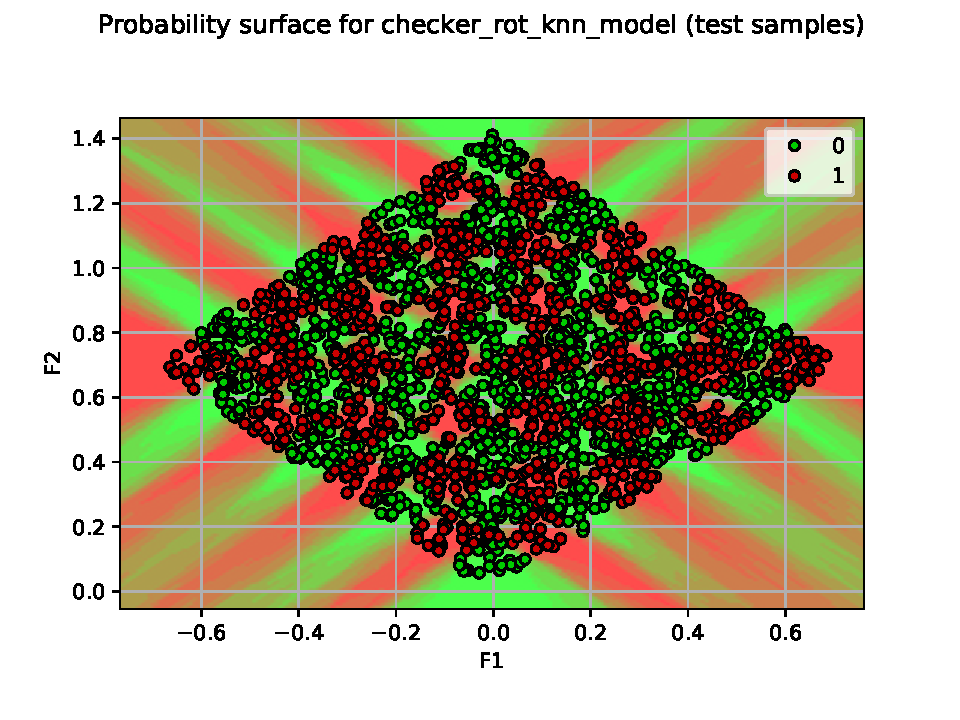
\includegraphics[width=0.49\textwidth]{figures/checker_rot_knn_surf_test.pdf}}
\subfloat[\textbf{XGBoost on the rotated checkerboard}]{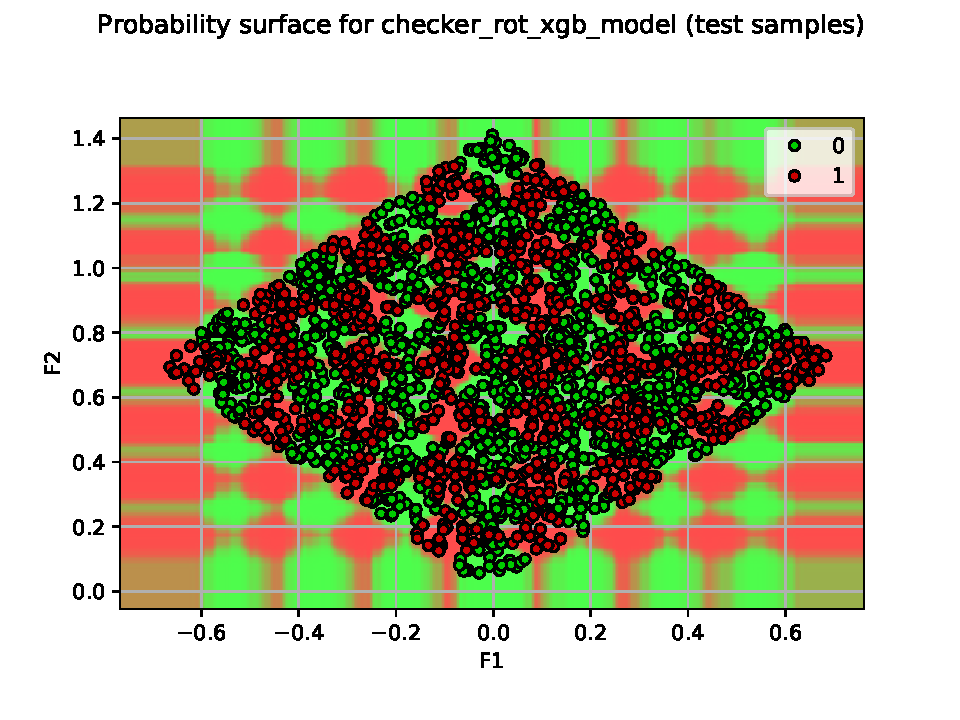
\includegraphics[width=0.49\textwidth]{figures/checker_rot_xgb_surf_test.pdf}}\\
\subfloat[\textbf{proset on the rotated checkerboard}]{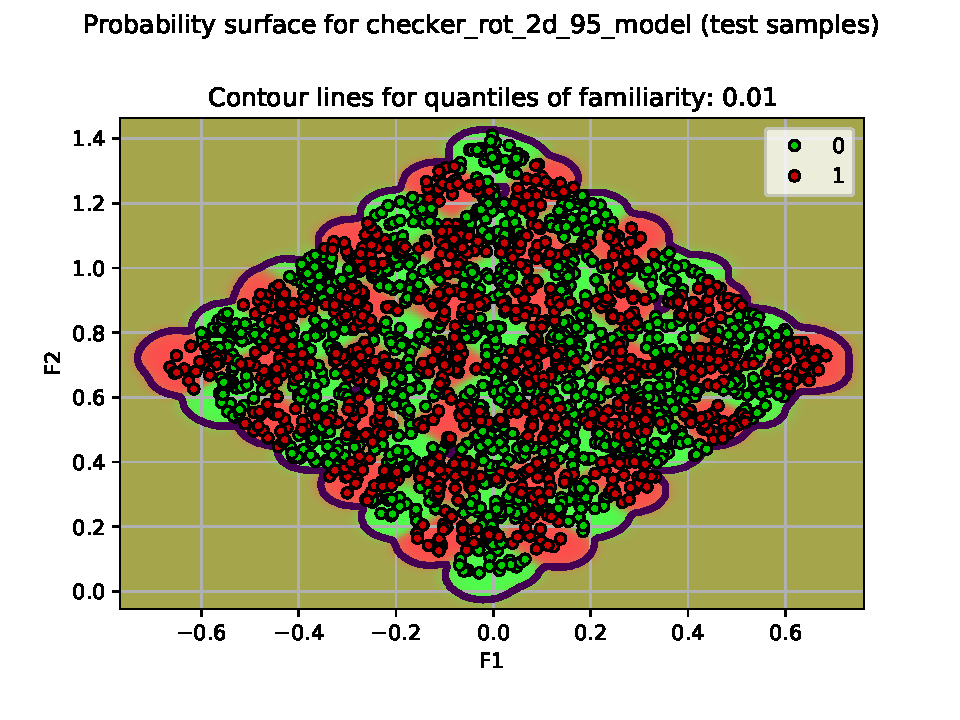
\includegraphics[width=0.49\textwidth]{figures/checker_rot_surf_test.pdf}}
\end{center}
\end{figure}
%
One problem faced by all machine learning is that their behavior becomes arbitrary for samples that are far removed from the original training data.
The way a model extrapolates outside its `area of competence' depends entirely on the specific algorithm and does not reflect any empirical evidence.
This is illustrated in Figure \ref{fig_area_of_competence} for the rotated checkerboard example.
The plots show the probability surfaces for each of the three classifiers studied in Section \ref{sec_classifier_comparison}, i.e., the color scale represents the estimated probability for class 1 from green (0.0) to red (1.0).
While kNN and XGBoost create idiosyncratic patterns in regions of the feature space with no training data, proset reverts to the marginal distribution.
The proset estimate is no more correct than that of the other two algorithms, but we consider it the most `honest' in the absence of information.
For balanced training data as in the example, proset does not assign a high probability to an arbitrary class as may happen with kNN or XGBoost.
Given that users tend to interpret the probability of the class with the highest probability estimate as the model's `confidence' in the result, this is an important advantage.\par
%
The proset algorithm can even provide an explicit indicator that a new sample is far away from the training data.
For any $x\in\R^D$, we define the familiarity of a proset model with $x$ as
%
\begin{equation}
\mathfrak{f}(x):=\sum_{b=1}^B\sum_{j=1}^{J_b}w_{b,j}G_{v_b}(x-x_{s_{b,j}})\label{eq_familiarity}
\end{equation}
%
This is just the denominator of (\ref{eq_pkx}) minus 1, which can be provided alongside the estimate with no additional effort.
Familiarity measures the total contribution of the weighted prototypes to the estimate relative to the marginal distribution represented by the 1.\par
%
Instead of using the absolute size of $\mathfrak{f}(x)$ to assess new samples, we find it more useful to express it as a quantile of the distribution of familiarity observed for test data.
As the model may overfit its training data slightly, it is better to use held-out data for this analysis.
Figure \ref{fig_area_of_competence} shows the resulting 1 \% contour line of familiarity for the proset classifier.
For a new sample, familiarity expressed as a quantile of the previously observed distribution can be interpreted as p-value of a statistical test whether the estimate is inside the model's `area of competence'.\par
%
For a supervised learning problem with many features, the training data is typically close to a `thin' manifold in the high-dimensional feature space.
Using quantiles of familiarity as indicated above, we can measure proximity to that manifold via a scalar indicator.
This is a powerful tool for monitoring a machine learning model in production and to detect data drift.
However, there is a trade-off between feature selection and the usefulness of familiarity.
Consider the case where proset does not select a feature because of insufficient variation in the training data.
A new sample that has a markedly different value in that one feature is still assigned a high familiarity score if the features actually used by the model lie in the expected range.\par
%
\begin{figure}
\caption{Familiariy of `easy' and `hard' test samples for MNIST}
\label{fig_mnist_familiarity}
%
\begin{center}
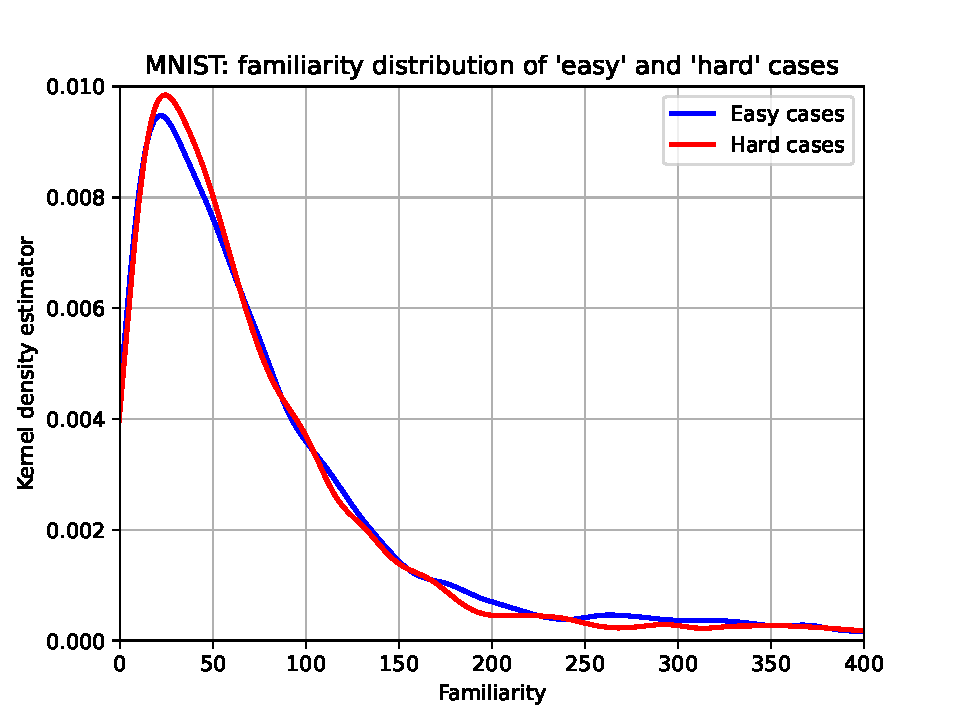
\includegraphics[width=0.49\textwidth]{figures/mnist_familiarity.pdf}
\end{center}
\end{figure}
%
\begin{table}
\caption{Difficulty and familiarity for MNIST data}
\label{tab_mnist_familiarity}
%
\begin{center}
\small
\begin{tabular}{|lrrrrr|}
\hline
&&\multicolumn{2}{c}{\textbf{Difficulty}}&\multicolumn{2}{c|}{\textbf{Familiarity}}\\
\textbf{Metric}&\textbf{Overall}&\textbf{Easy}&\textbf{Hard}&\textbf{High}&\textbf{Low}\\
Log-loss$^*$&0.23&0.17&0.28&0.10&0.35\\
ROC-AUC&1.00&1.00&1.00&1.00&0.99\\
Balanced accuracy&0.95&0.97&0.94&0.98&0.91\\
\multicolumn{6}{|l|}{$^*$ The equivalence threshold for the overall fit is 0.26, so the}\\
\multicolumn{6}{|l|}{\phantom{$^*$} `hard' or `unfamiliar' cases are strictly worse by our standard.}\\
\hline
\end{tabular}
\end{center}
\end{table}
%
As further example, we look a MNIST data, where we know that test samples submitted by high-school students are harder to classify than those by Census Bureau employees.
It is interesting to consider whether this can be detected using the familiarity score.
While the training data is sampled from both groups, we might expect that regularly formed digits generalize better and are preferred as prototypes.
In turn, other regular digits would appear more familiar.
Figure \ref{fig_mnist_familiarity} shows the familiarity distribution for each group as a kernel density plot.
Results are based on the best proset model fitted to MNIST data (PCA features with no prior scaling, cp.\ Section \ref{sec_timing_larger_cases}).
Note that the plots shows `raw' values instead of quantiles and excludes the right tails to focus on the modes of the distribution.
The expected effect is visible -- there are more `hard' cases with a familiarity below 60 - but it is not very pronounced.\par
%
Another interesting question is whether the model performs better on `familiar' cases.
Table \ref{tab_mnist_familiarity} shows metrics for the entire test data set, the `easy' and hard' cases, as well as the top and bottom half of samples ranked by familiarity.
The effect of splitting based on familiarity is greater than splitting the two groups of writers.
This suggests that familiarity could be used to gauge predictions in a process where some cases are submitted for human review.
While not suitable for optical character recognition, the approach could benefit other applications.
%
\section{Explaining individual estimates}
\label{sec_individual_explanations}
%
\subsection{Explanation report}
\label{sec_explanation_report}
%
\begin{figure}
\caption{Example of explanation report for cancer data}
\label{fig_explanation_report}
%
\begin{center}
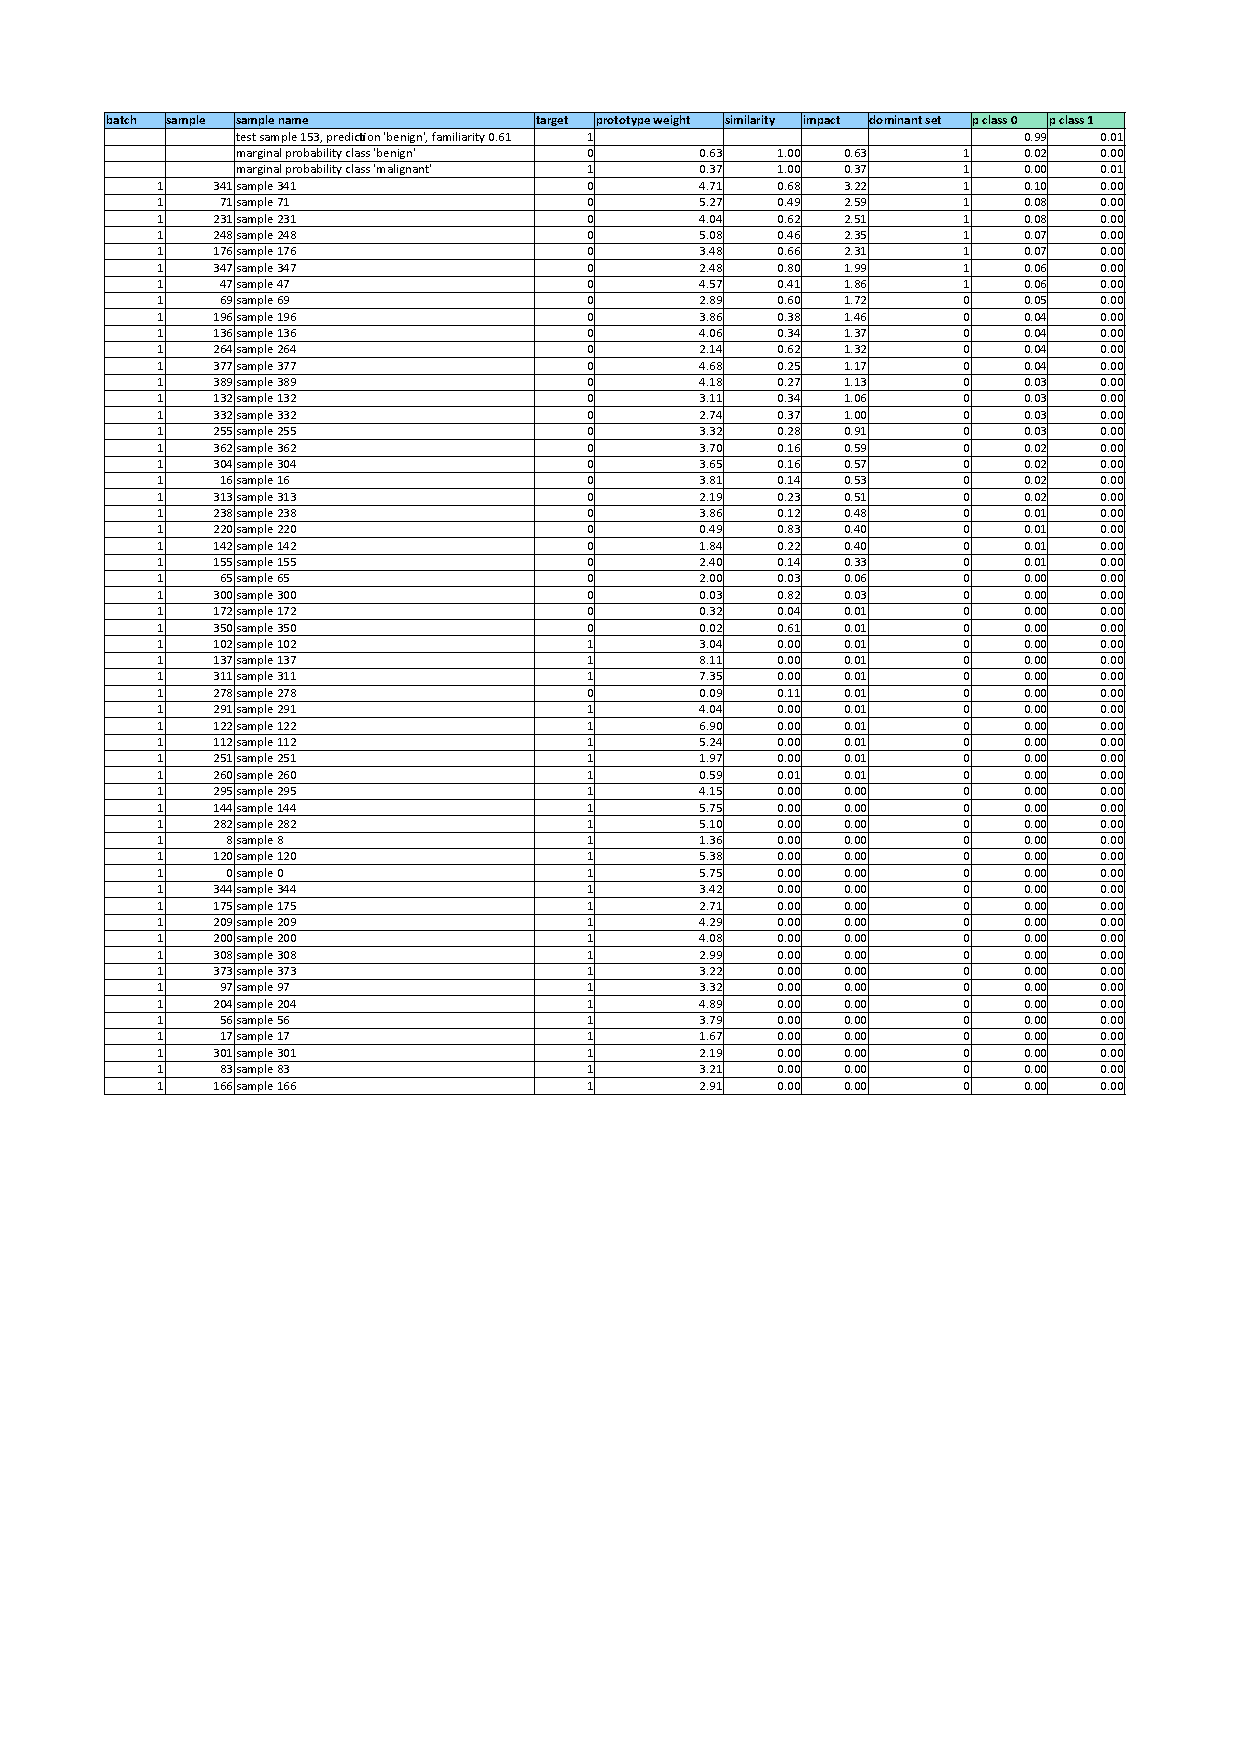
\includegraphics[width=0.95\textwidth, trim={1.5cm 2.0cm 1.5cm 1.5cm}, clip]{figures/cancer_2d_95_model_explain.pdf}
\end{center}
\end{figure}
%
Our implementation of proset can export information about the model as tabular data.
The basic report contains information on all prototypes, their weights, and active features.
A more interesting report relates a particular sample to the selected prototypes.
Figure \ref{fig_explanation_report} shows an example analysis for the proset classifier.
It deals with the one misclassified `malignant' case from the cancer data example that is surrounded by `benign' cases.
The report contains the following information:
%
\begin{description}
\item[Batch:] the number of the batch to which each prototype belongs.
The model in the example has only a single batch.
The first three rows contain information on the misclassified sample and the marginal distribution, they are not associated with any batch.
%
\item[Sample:] the zero-based index of the prototype with respect to the ordering of the training data after the train-test split.
%
\item[Sample name:] the record for the test sample states its zero-based index within the set of test data, the class with the highest estimated probability, and familiarity expressed as a quantile of the distribution for the test data.
The remaining rows indicate whether they belong to the marginal distribution or individual prototypes.
%
\item[Target:] the numeric representation of the class, either 0 (`benign') or 1 (`malignant').
The first rows contains the true target for the test sample.
%
\item[Prototype weight:] the value $w_{b,j}$ for each prototype.
The test sample has no entry, records for the marginal distribution show the marginal probability for the corresponding class.
%
\item[Similarity:] the value of the unnormalized Kernel $G_{v_b}$ at $x-x_{s_{b,j}}$.
This is a number in $(0,1]$, where $1$ indicates that the sample features $x$ are identical to those of the prototype.
The test sample has no entry, records for the marginal probabilities list a 1 as they affect all estimates equally.
%
\item[Impact:] the product of prototype weight and similarity is the total impact of the prototype on the estimated probability (\ref{eq_pkx}).
By default, the report lists the prototypes in order of descending impact.
%
\item[Dominant set:] a binary indicator of observations that have the largest impact on the estimate.
The target values for prototypes outside the dominant set can be changed without affecting which class is assigned the highest probability.
See below for a precise definition of the dominant set.
%
\item[p class 0:] the record for the test sample shows the estimated probability for class 0 (`benign').
The remaining rows contain the additive contribution of the marginal distribution and prototypes to this estimate.
The contribution is equal to the impact listed for the row divided by the total impact if the target is 0.
Otherwise, the contribution is zero.
%
\item[p class 1:] as above for class 1 (`malignant').
\end{description}
%
The report provides a complete breakdown of the estimate for one sample into the contribution of the marginals and prototypes.
The multivariate structure of the feature space is replaced by a simple list that can be filtered and sorted by different criteria to identify major contributors.
While the total number of prototypes can be much larger than in the example, most tend to have negligible impact on any particular case.\par
%
For the computation of the `dominant set' indicator, we use the following procedure:
%
\begin{algorithm}[Dominant set]~
\label{alg_dominant_set}
%
\begin{enumerate}
\item Sort the prototypes in descending order of impact and assign a rank to each.
Prototypes with the same impact receive the same rank.
%
\item For each rank $r$, compute $p_{r,k}$ as sum of additive contributions (columns `p class 0', etc.\ in the report) to the probability estimate for class $k$ from the marginal distribution and prototypes up to rank $r$.
These satisfy $0<\sum_{k=0}^{K-1}p_{r,k}\leq 1$.
The remainder $t_r:=1-\sum_{k=0}^{K-1}p_{r,k}$ is the total contribution of prototypes with rank greater than $r$.
%
\item For each rank $r$, denote by $k_{1,r}$ and $k_{2,r}$ the classes with the largest and second largest value of $p_{r,k}$.
Determine the set  $R:=\{r:p_{r,k_{1_r}}-p_{r,k_{2,r}}>t_r\}$.
%
\item If $R$ is empty, the dominant set is empty.
Otherwise, all prototypes with a rank less than or equal to the minimal element in $R$ form the dominant set.
\end{enumerate}
\end{algorithm}
%
\begin{remark}
By constructions, if $R$ is not empty, it contains all ranks greater than or equal to its minimal element and all share the same value for $k_{1,r}$.
Thus, it contains all ranks where the remainder $t_r$ is too small to affect which class is assigned the highest probability.
\end{remark}
%
In the example report, the prototypes of the dominant set together with the marginal distribution contribute 53 percentage points of the 99 \% probability estimated for class 0.
Thus, class 0 would be assigned the highest probability even if all remaining prototypes belonged to class 1.
The purpose of the dominant set is to serve as a guideline which prototypes need to be reviewed for a better understanding of a particular result.\par
%
\begin{figure}
\caption{`Batch 1 map' of cancer data showing prototype impact}
\label{fig_batch_1_map_impact}
%
\begin{center}
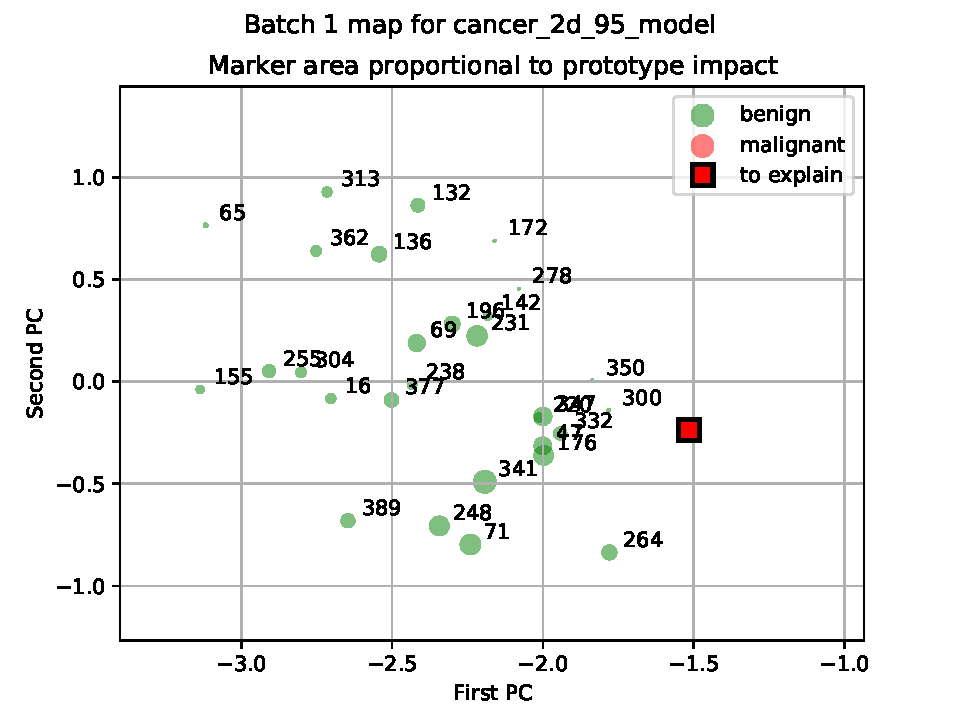
\includegraphics[height=0.4\textheight]{figures/cancer_batch_1_map_impact.pdf}
\end{center}
\end{figure}
%
The impact of prototypes on a particular estimate can also be visualized in the `batch 1 map'.
Figure \ref{fig_batch_1_map_impact} does this for the case from the example report.
The size of each circle is proportional to the impact of the prototype, numbers refer to the sample index.\par
%
\begin{figure}
\caption{Explanation using prototypes for CIFAR-10 data}
\label{fig_prototypes_cifar-10}
%
\begin{center}
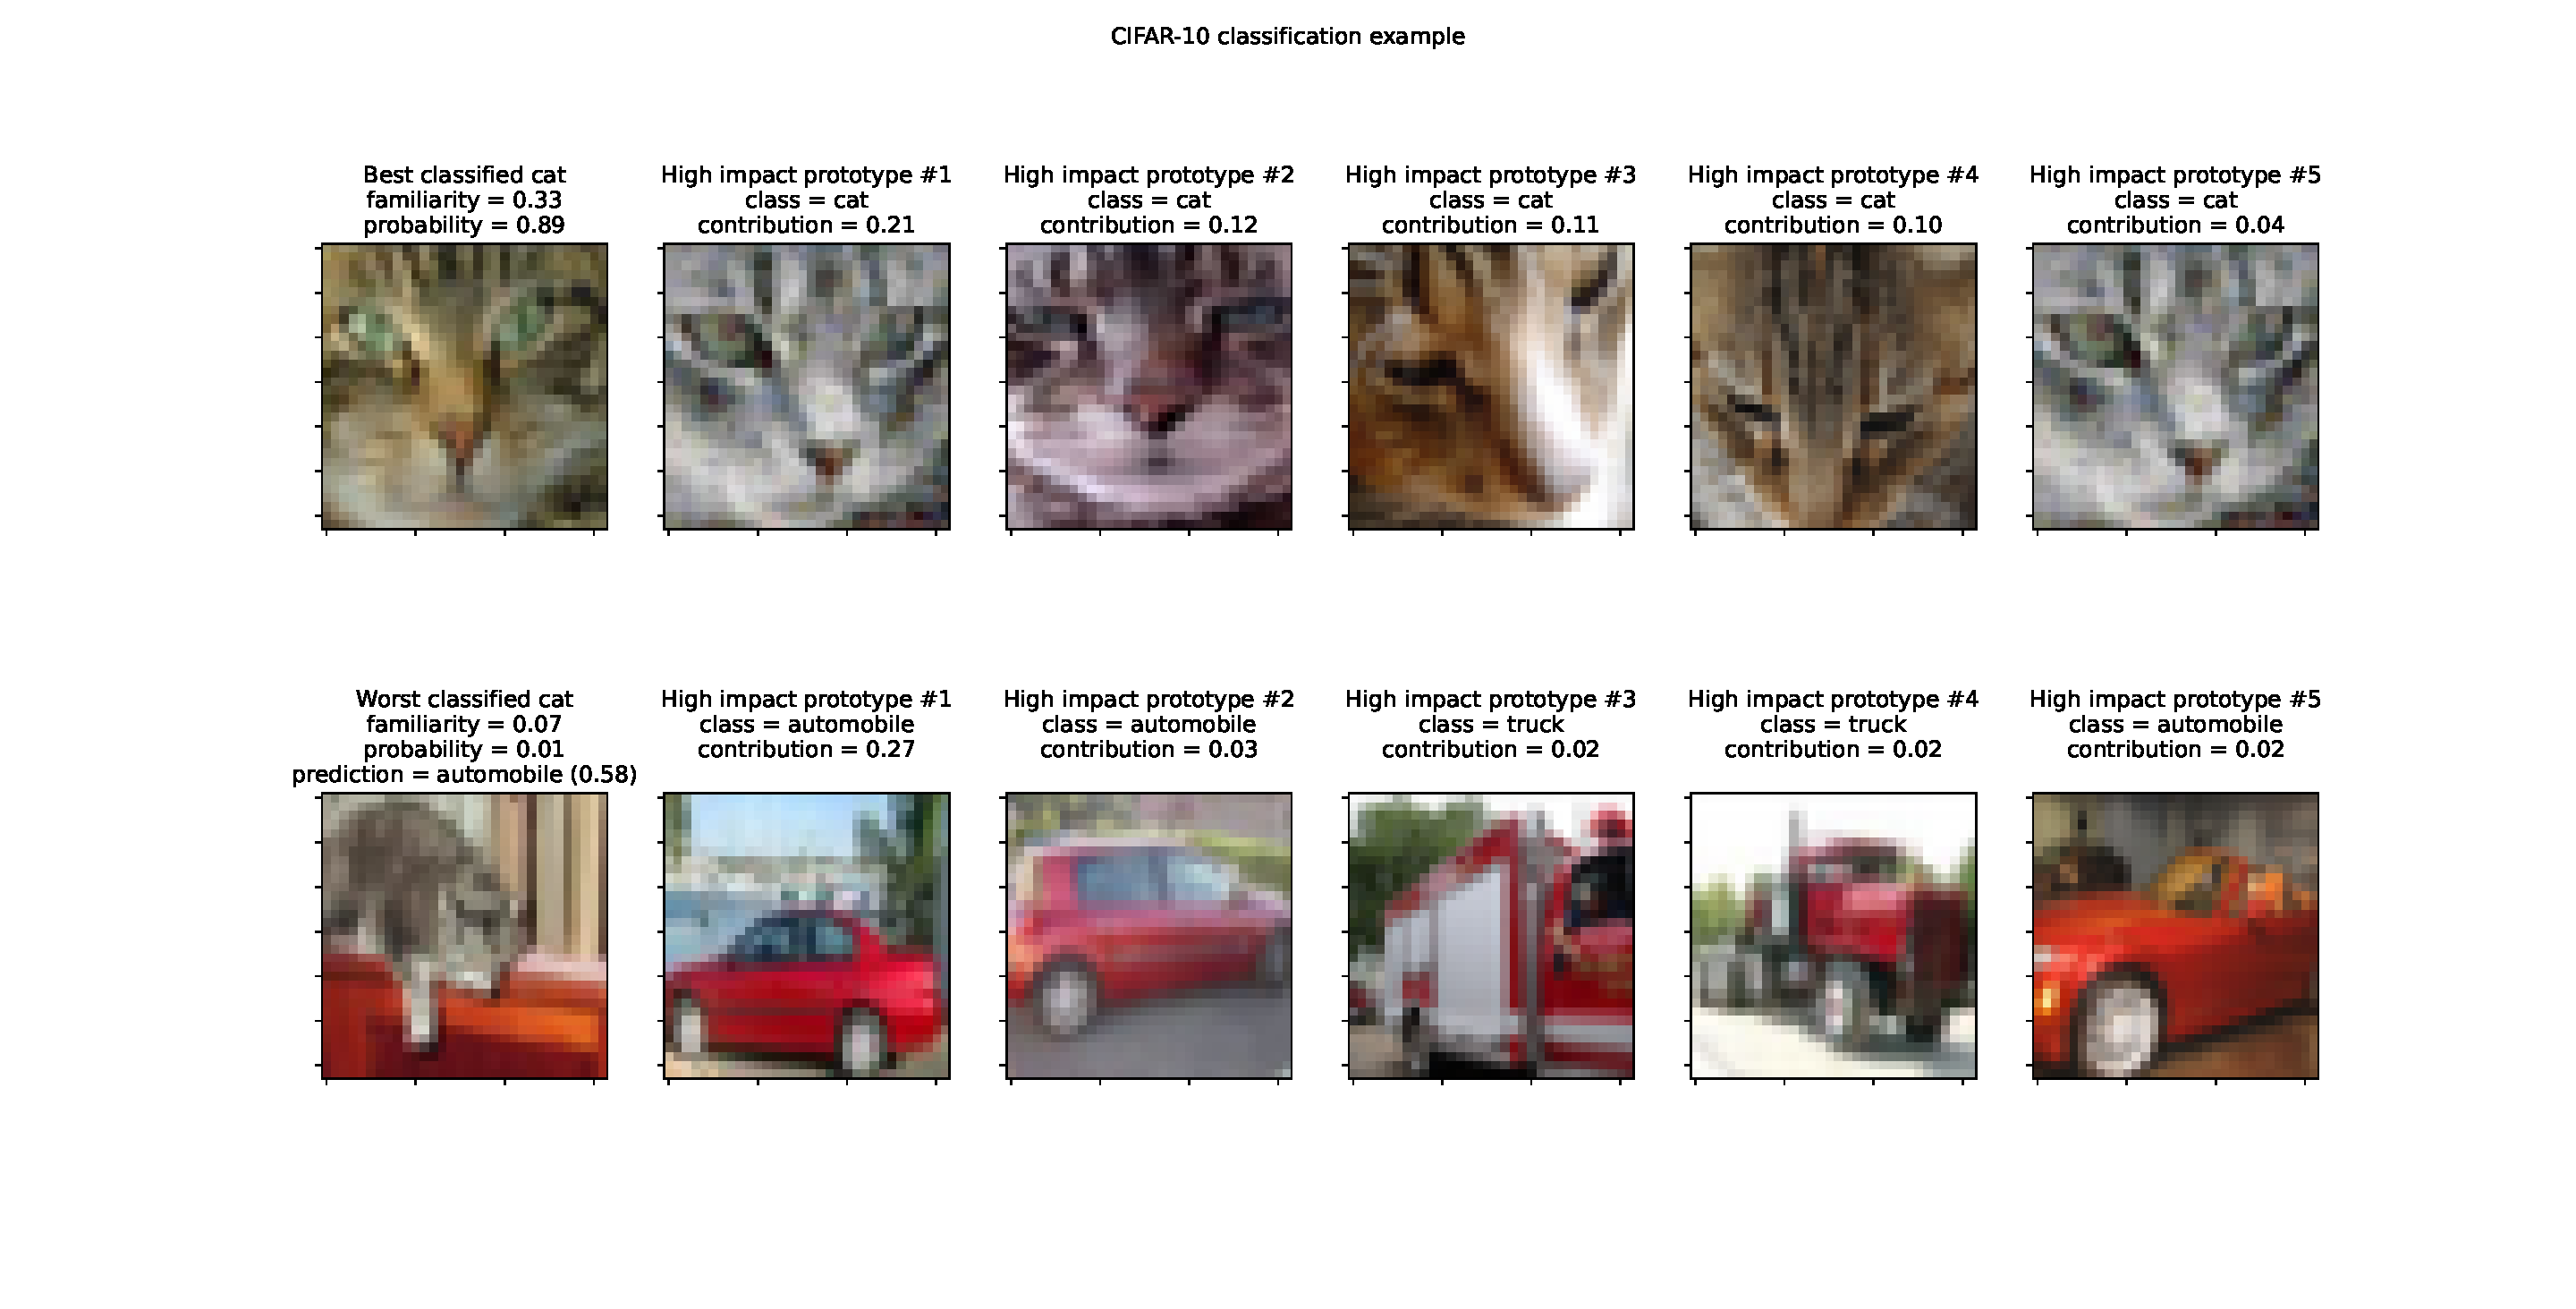
\includegraphics[width=0.9\textheight, angle=90, trim={1.5cm 1.5cm 1.5cm 0.5cm}, clip]{figures/cifar-10_model_explain.pdf}
\end{center}
\end{figure}
%
While it is daunting to look at individual features for the CIFAR-10 data, we can still explain a prediction in terms of images selected for prototypes.
Proset does not perform well on this data set (cp.\ Section \ref{sec_timing_larger_cases}), but it provides a good illustrative example.
Figure \ref{fig_prototypes_cifar-10} shows the two test images of cats achieving the highest and lowest predicted probability for the true class.
The `reasoning' behind the predictions is explained by including for each case the images corresponding to the five prototypes with the most impact.\par
%
The first image is classified as a cat with an estimated probability of 89 \%.
It shows a close-up of the cat's face with no distracting background.
The five prototype images all show cat faces from different angles.
Note that the first and fifth prototype represent the same image in different batches, so the relevant features are likely to differ as well.
The first four prototypes form the dominant set of this prediction.
Together, they contribute 54 percentage points to the estimated probability and determine the majority class.\par
%
The second image is classified as an automobile with a probability of 58 \%, with an estimate of only 1 \% for a cat.
In this case, the animal is shown from farther away and its face is not clearly visible.
Even worse, the background seems to be more distinctive than the main object.
The cat rests on a piece of red furniture with a horizontal groove whose feature representation apparently resembles a red car or truck.
As a consequence, the most similar prototypes all belong to these two classes.
The first prototype contributes 27 percentage points to the estimated for class automobile.
All others have a small contribution each, but there are many more before the first cat appears in the ranked list.
%
\subsection{Combining SHAP values and geometric analysis}
\label{sec_shap_values}
%
So far, we have looked at model-specific explanations for proset estimators on their own.
In this section, we combine them with a model-agnostic approach to gain additional insight into the model structure.
We choose the SHAP (SHapley Additive exPlanations) method for assessing feature importance proposed by Lundberg and Lee \cite{Lundberg_17}.
SHAP provides explanations for individual estimates and is the only additive feature attribution method that has certain desirable properties.
A downside is that the computational effort grows exponentially in the number of features, although an efficient algorithm exists for decision trees \cite{Lundberg_18}.
To facilitate usage of SHAP, our implementation of proset allows `shrinking' the model to take only the features with nonzero weights as input.\par
%
SHAP explains an estimate by comparing the sample of interest to a reference point.
The relative change in the estimator between the points is attributed to the relative change in the features.
There appears to be little research so far on the best choice of reference point, but Izzo et.\ al.\ \cite{Izzo_20} consider the issue.
The authors point out that the common choice of using the origin of the feature space as baseline is not satisfactory.
For a binary classifier, they recommend to select a reference point on the decision boundary between the two classes.
They refer to this as a `neutral baseline', since the algorithm is indifferent which class to choose.
We cannot follow this approach, as we want to study the probability estimate itself without reference to a decision rule\footnote{
We do use the `naive' decision rule that selects the class with the highest estimated probability to define bins for Algorithm \ref{alg_bins} and to compute balanced accuracy as a secondary metric for the benchmark study.
See the discussion in the next paragraph why we do not consider this rule for further analysis.
}.
Also, several of the benchmark cases have more than two classes and it is not certain that a point can be found that is `neutral' with regards to all of them at once.\par
%
We believe that classification should always be carried out in two stages by combining a stochastic model with a decision rule.
The purpose of the former is to accurately estimate the probability distribution with no regard to the practical problem we want to solve.
The purpose of the latter is to optimize the expected value of a problem-specific utility or loss function under the estimated distribution.
Any algorithm that conflates the two stages implicitly applies an arbitrary decision rule that is likely to yield sub-optimal results.
As an example, consider a credit scoring algorithm that estimates the default probability for loans.
It is doubtful that the lending company wants to grant loans to all applicants with default probability less than 50 \%.
A thorough discussion of this issue can be found, e.g., in a blog article by Frank Harrell \cite{Harrell_20}.\par
%
For the above reason, we want to find a suitable reference point for explaining the estimated probabilities themselves regardless of any decision rule that could be applied later.
We expect such a point to have the following three properties:
%
\begin{enumerate}
\item The point itself represents a feasible combination of features.
%
\item The point is not extreme in terms of the feature space.
For every feature, there are training samples that have either a higher or lower value.
%
\item The point is not extreme in terms of the estimated probabilities.
For every class, there are training samples that have either a higher or lower estimate.
\end{enumerate}
%
\begin{remark}
\begin{enumerate}
\item Property 1 acknowledges that the baseline is part of the explanation and should have no `unnatural' characteristics.
There is less risk of misinterpreting the feature importance if they are computed with respect to a relatable feature vector.
%
\item Properties 2 and 3 mean that SHAP can explore changes of the input and output in all directions.
%
\item Property 3 can be viewed as a weaker notion of the `neutral baseline' proposed in \cite{Izzo_20}.
%
\item Properties 1 and 2 are mutually exclusive for binary features.
Here, we prefer property 1, i.e., the baseline should be a genuine case and not a hypothetical half-way point.
\end{enumerate}
\end{remark}
%
One way to satisfy the first condition is to use an actually observed point as reference.
The first two conditions imply that a medoid\footnote{
A medoid is any point from a set for which the average absolute distances to all other points is minimal.
In one dimension, a medoid is also a median of the data.
} of the feature vectors for the training data is a suitable choice.
Likewise, condition 1 and 3 suggest to use a point whose estimated probabilities are a medoid of the probability vectors for the training data.
We thus propose the following procedure for choosing a baseline:
%
\begin{algorithm}[SHAP baseline]~
\label{alg_shap_baseline}
%
\begin{enumerate}
\item Rank all training samples in increasing order of average absolute distance to all other training samples in the feature space.
Use only features selected by proset to compute distances.
%
\item Rank all training samples in increasing order of average absolute distance to all other training samples in the space of estimated probability vectors.
%
\item Combine both rankings using Borda's rule\footnote{
Borda's rule converts rankings to scores by assigning each candidate half a point for each other candidate ranked the same, plus a full point for each candidate ranked worse.
Scores are totaled across rankings and the winners are the candidates with the most points.
} and use the winner as reference.
In case of a tie, choose the candidate whose probability vector has the highest entropy.
If still tied, use the point with the lowest sample index.
\end{enumerate}
\end{algorithm}
%
\begin{remark}
\begin{enumerate}
\item We do not recommend to combine the active features and estimated probabilities into a single vector.
The medoid property depends on the scaling of of individual variables and there is no obvious common scale.
Also, if there are many more features than classes, the former might dominate the decision.
Computing two separate rankings and using Borda's rule results in a choice that balances properties 2 and 3.
%
\item The method requires computing pairwise distances for all training samples, which may be unattractive for large problems.
In this case, we recommend subsampling.
\end{enumerate}
\end{remark}
%
\begin{figure}
\caption{`Batch 1 map' of cancer data showing reference point}
\label{fig_batch_1_map_reference}
%
\begin{center}
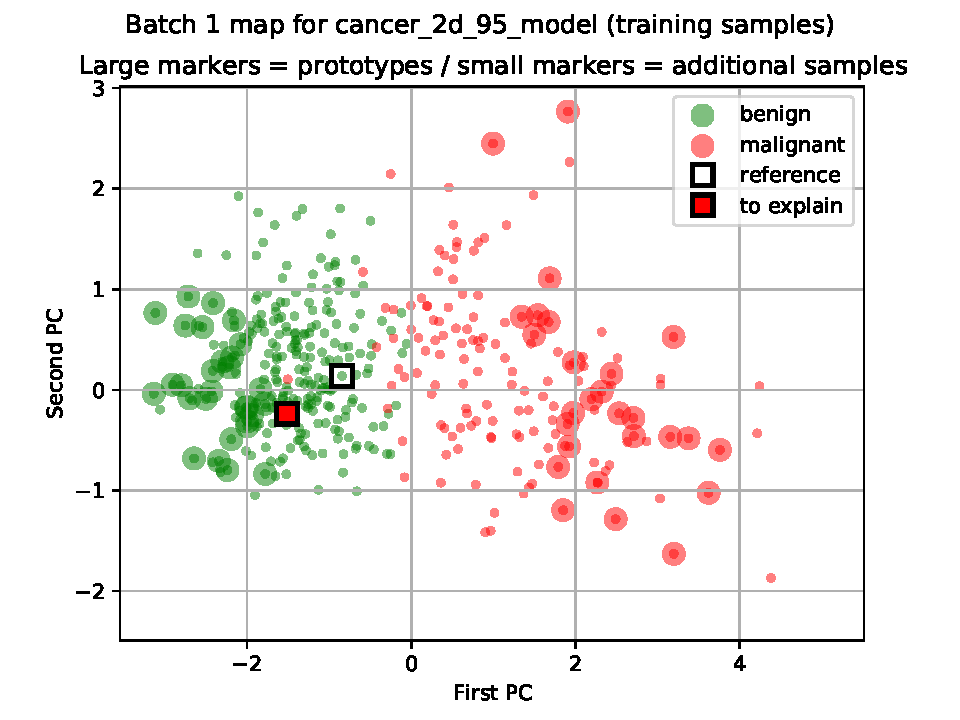
\includegraphics[height=0.4\textheight]{figures/cancer_batch_1_map_training_data_reference.pdf}
\end{center}
\end{figure}
%
\begin{figure}
\caption{SHAP feature importance}
\label{fig_feature_importance}
%
\begin{center}
\subfloat[\textbf{Global importance}]{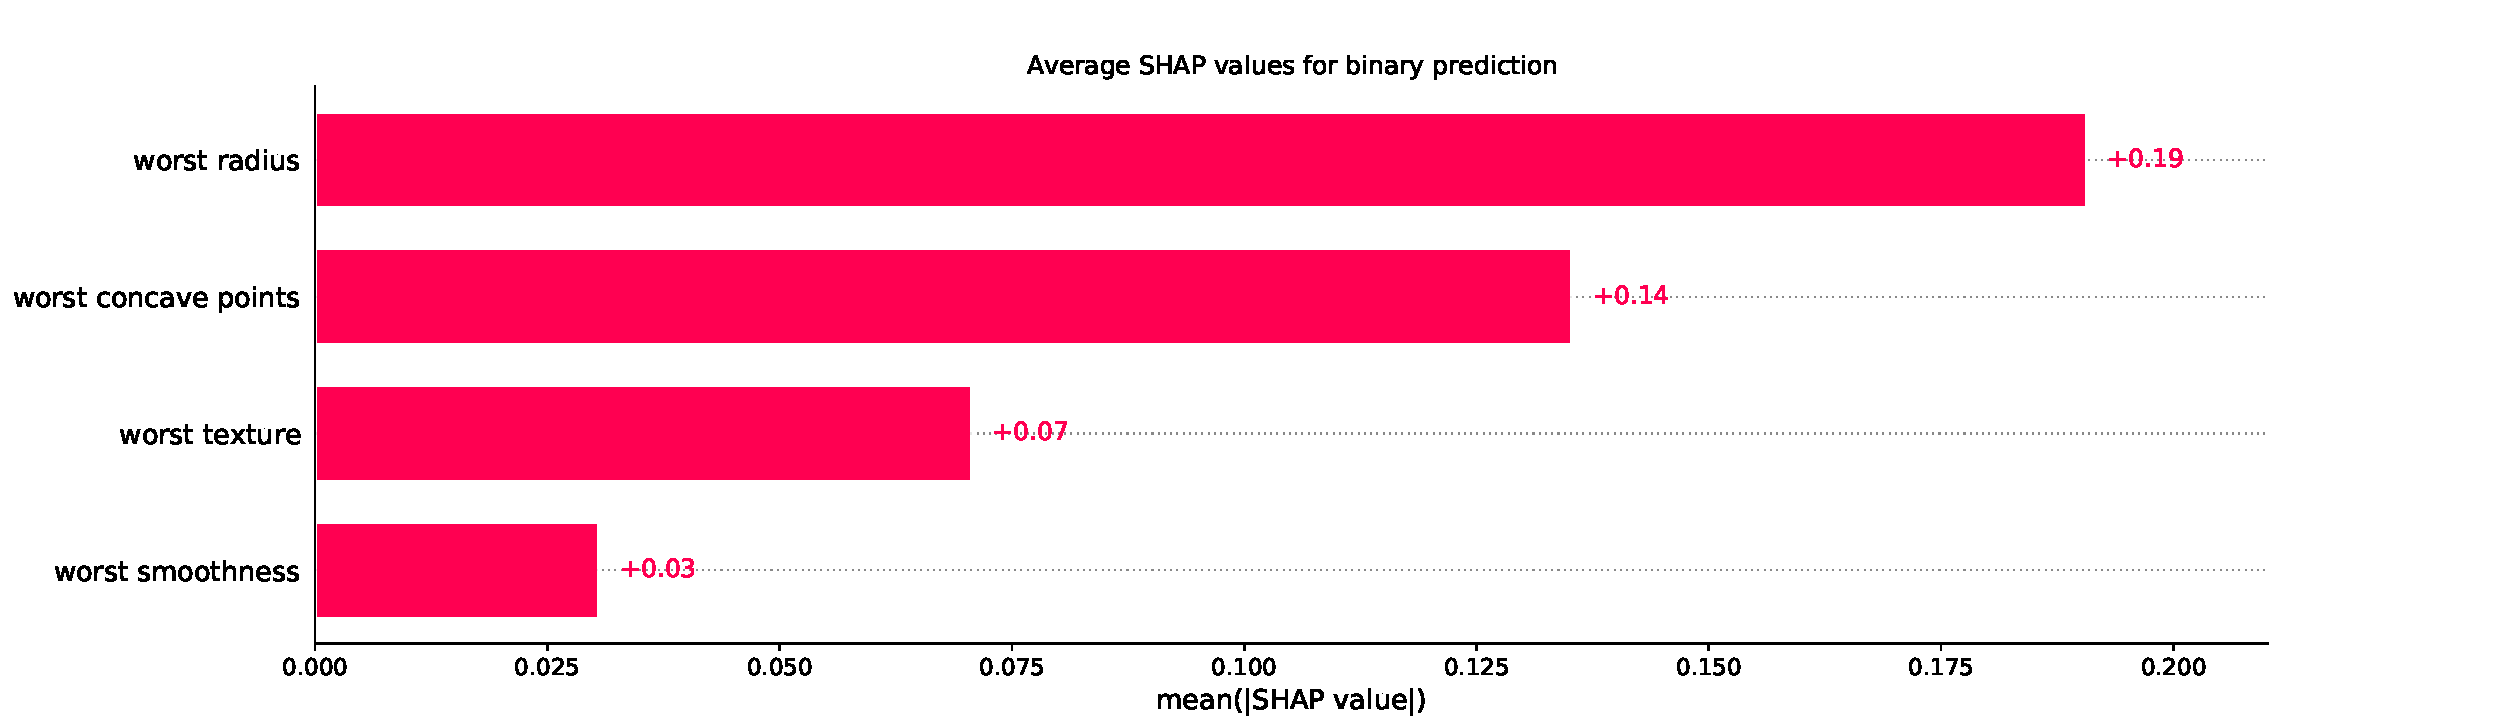
\includegraphics[width=0.99\textwidth]{figures/cancer_global_shap.pdf}}\\
\subfloat[\textbf{Misclassified case}]{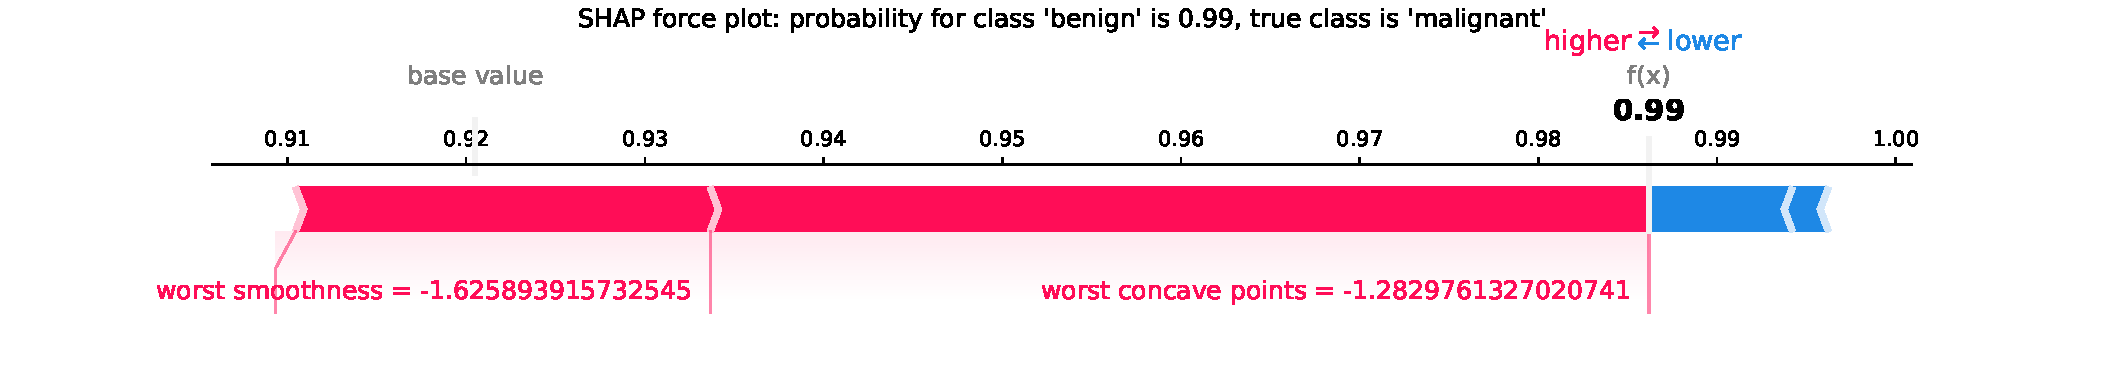
\includegraphics[width=0.99\textwidth]{figures/cancer_example_shap.pdf}}
\end{center}
\end{figure}
%
\begin{figure}
\caption{Scatter plots for important features}
\label{fig_scatter_important}
%
\begin{center}
\subfloat[\textbf{Global importance}]{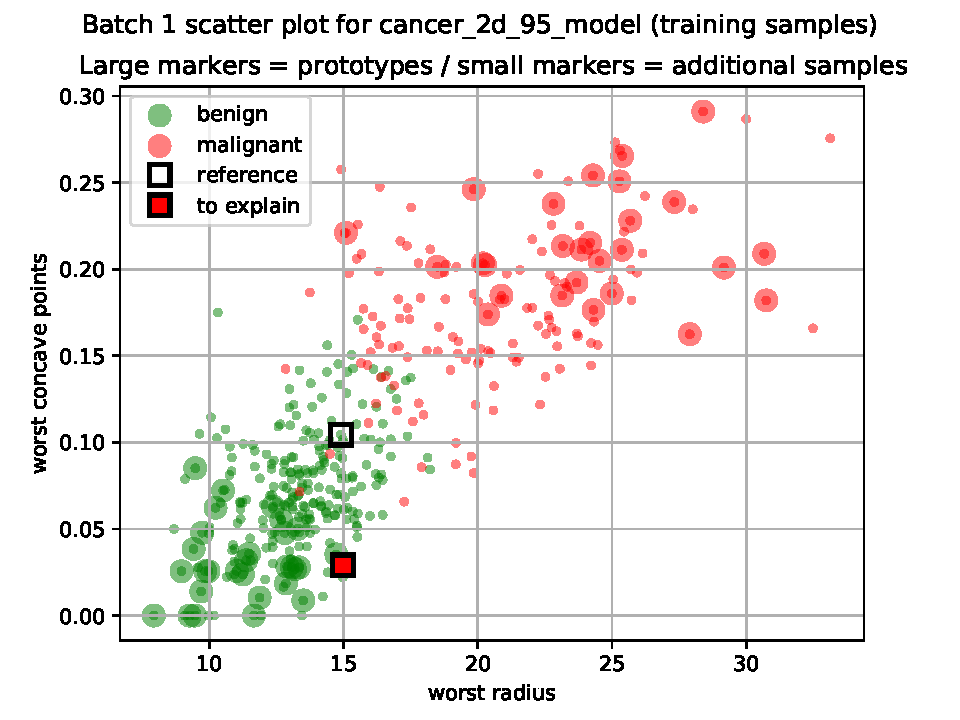
\includegraphics[height=0.4\textheight]{figures/cancer_scatter_global_shap.pdf}}\\
\subfloat[\textbf{Misclassified case}]{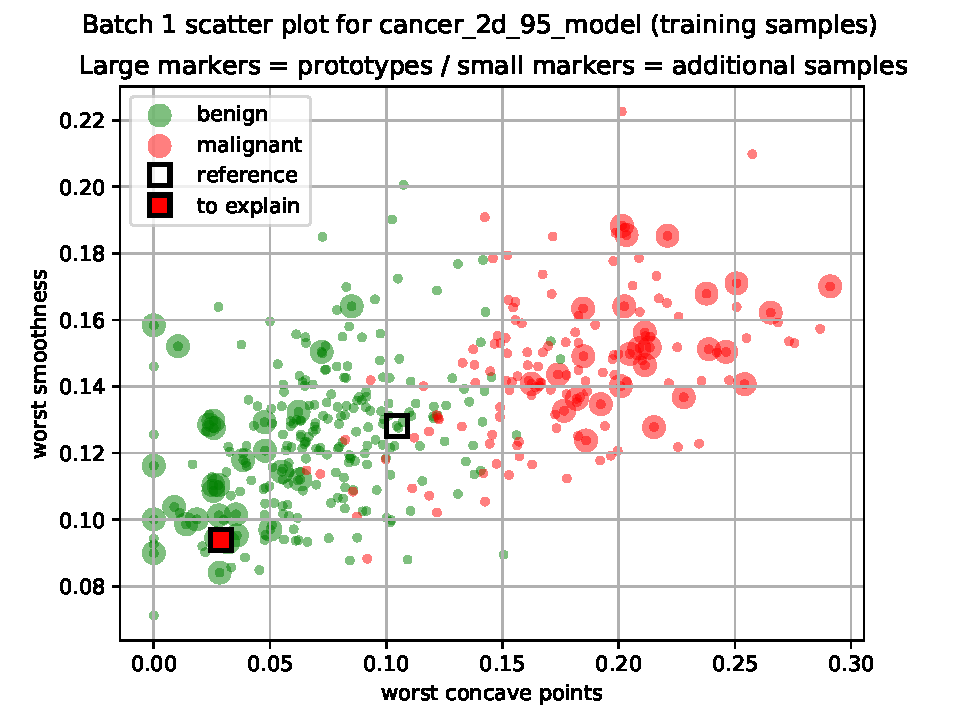
\includegraphics[height=0.4\textheight]{figures/cancer_scatter_example_shap.pdf}}
\end{center}
\end{figure}
%
\begin{figure}
\caption{Probability surfaces for important features}
\label{fig_probability_important}
%
\begin{center}
\subfloat[\textbf{Global importance}]{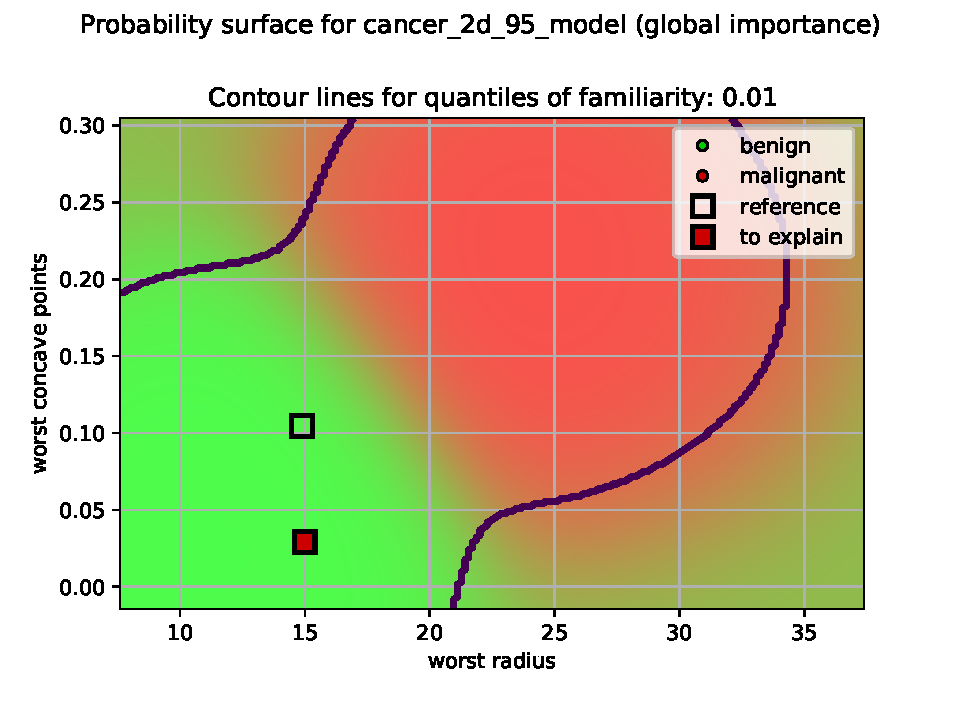
\includegraphics[height=0.4\textheight]{figures/cancer_surface_global_shap.pdf}}\\
\subfloat[\textbf{Misclassified case}]{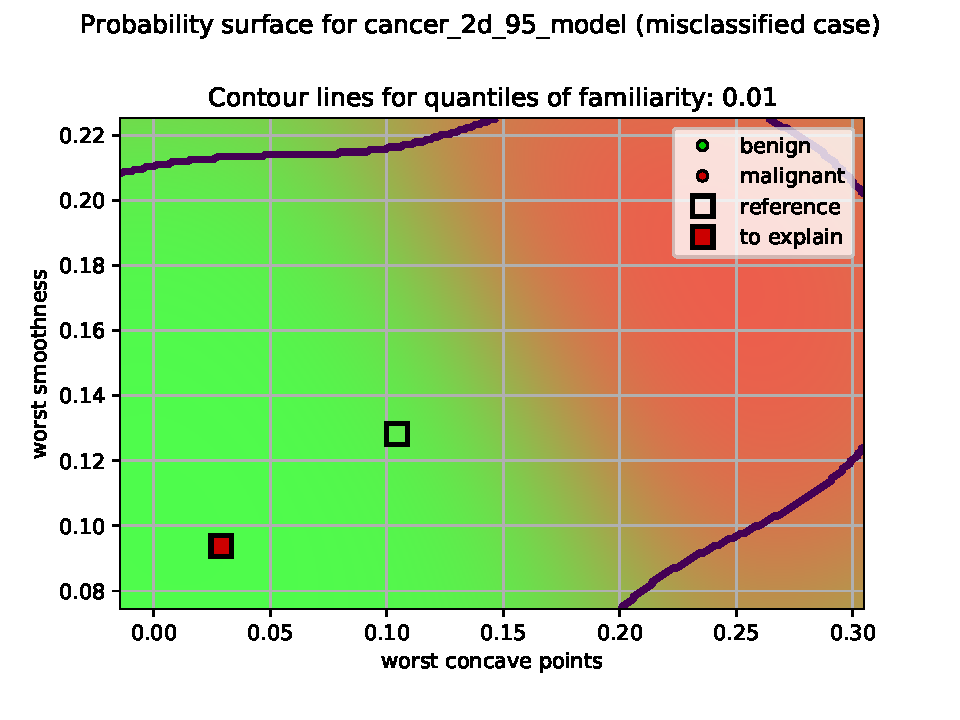
\includegraphics[height=0.4\textheight]{figures/cancer_surface_example_shap.pdf}}
\end{center}
\end{figure}
%
If we apply the above rule to the cancer data, it selects a baseline near the center of the point cloud of training samples.
The estimated probability for being `benign' is 92 \%, which is far from the 50 \% that would be achievable given the structure of the data.
However, the data is unbalanced in favor of `benign' cases and we have seen for the misclassified case in the previous section that probabilities in excess of 92 \% are achievable.
Figure \ref{fig_batch_1_map_reference} shows the reference point in a `batch 1 map' together with training data and the misclassified case we want to explain.\par
%
Figure \ref{fig_feature_importance} shows the results of SHAP analysis for the whole test data and the misclassified case.
Note that the global values are just the averages of the absolute scores of each feature across all samples.
Ordering the features by descending global importance yields the same sequence as for the feature weights, but we do not believe that this necessarily holds for every data set.
The two most important features globally are `worst radius' and `worst concave points'.
For the misclassified case, the estimate for class `benign' is shifted from 92 \% (baseline) to 99 \% because of the extremely low values for `worst concave points' and `worst smoothness'.
Figure \ref{fig_scatter_important} shows the bivariate scatter plots for both pairs of features, this time with training data as supplementary information.
As an alternative, we can study the probability surface resulting for the most important features if the other features are fixed at their values for the misclassified case.
This is shown in Figure \ref{fig_probability_important}.\par
%
\begin{figure}
\caption{`Batch 1 map' for digits data showing test samples}
\label{fig_batch_1_map_test_digits}
%
\begin{center}
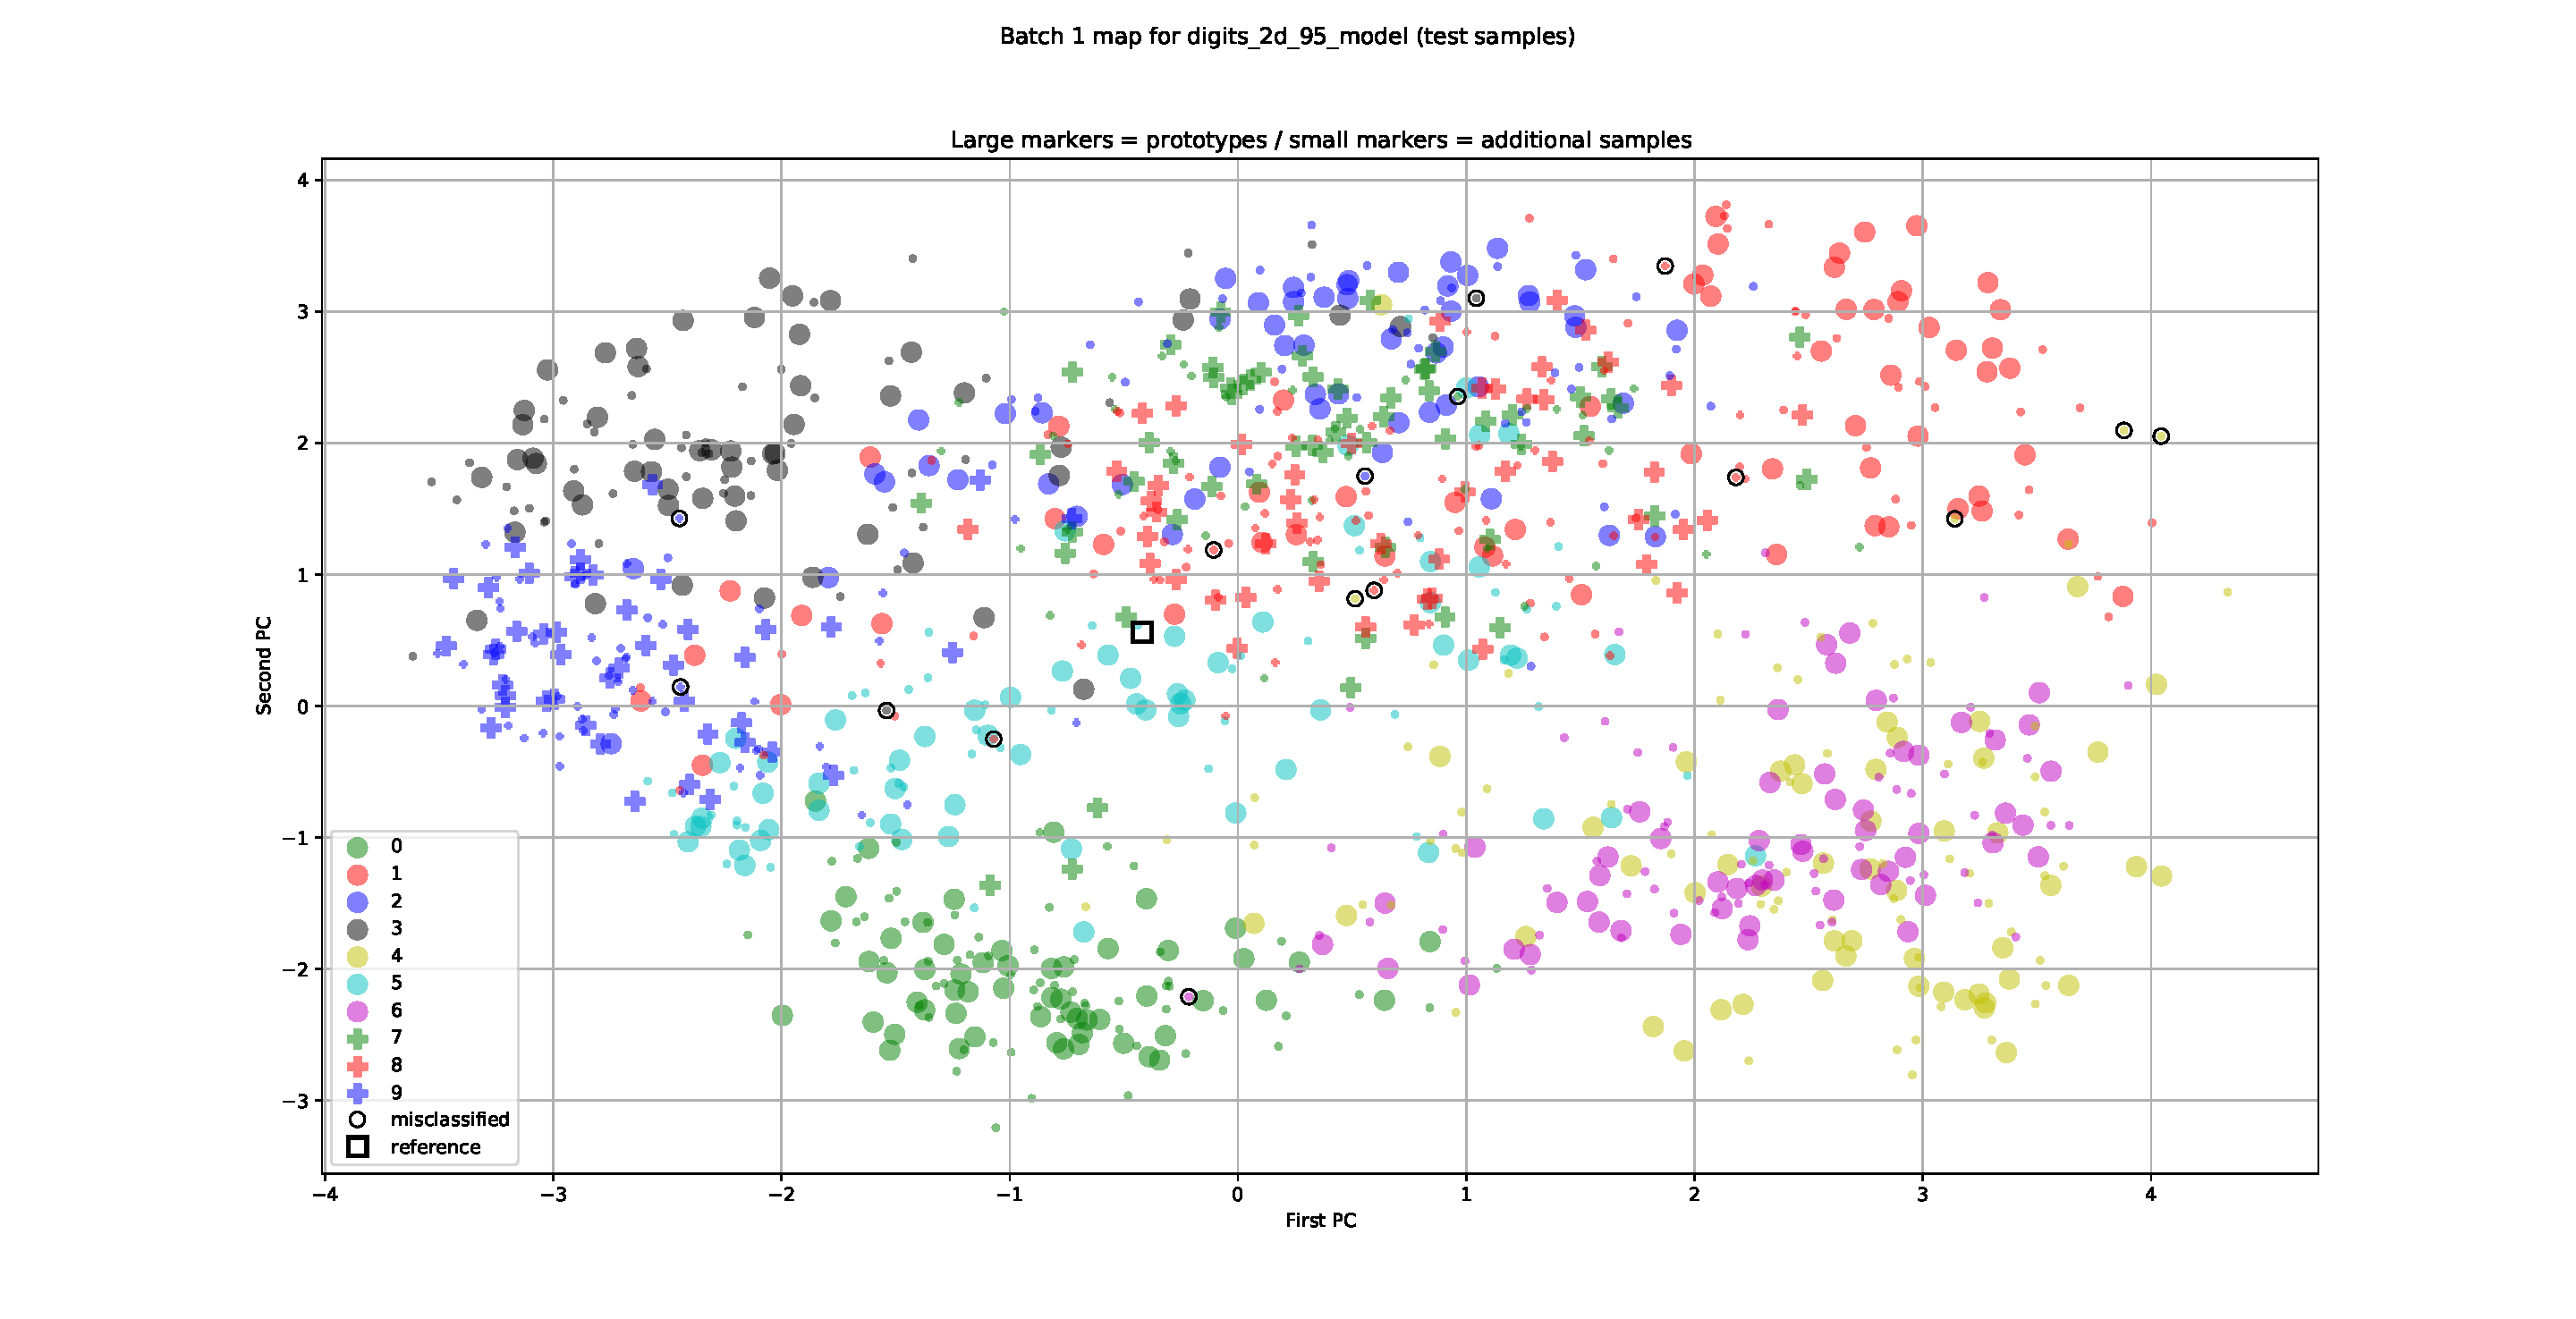
\includegraphics[width=0.9\textheight, angle=90, trim={1.5cm 1.5cm 1.5cm 0.5cm}, clip]{figures/digits_batch_1_map.pdf}
\end{center}
\end{figure}
%
\begin{figure}
\caption{Explanation combining prototypes and SHAP values}
\label{fig_impact_shap}
%
\begin{center}
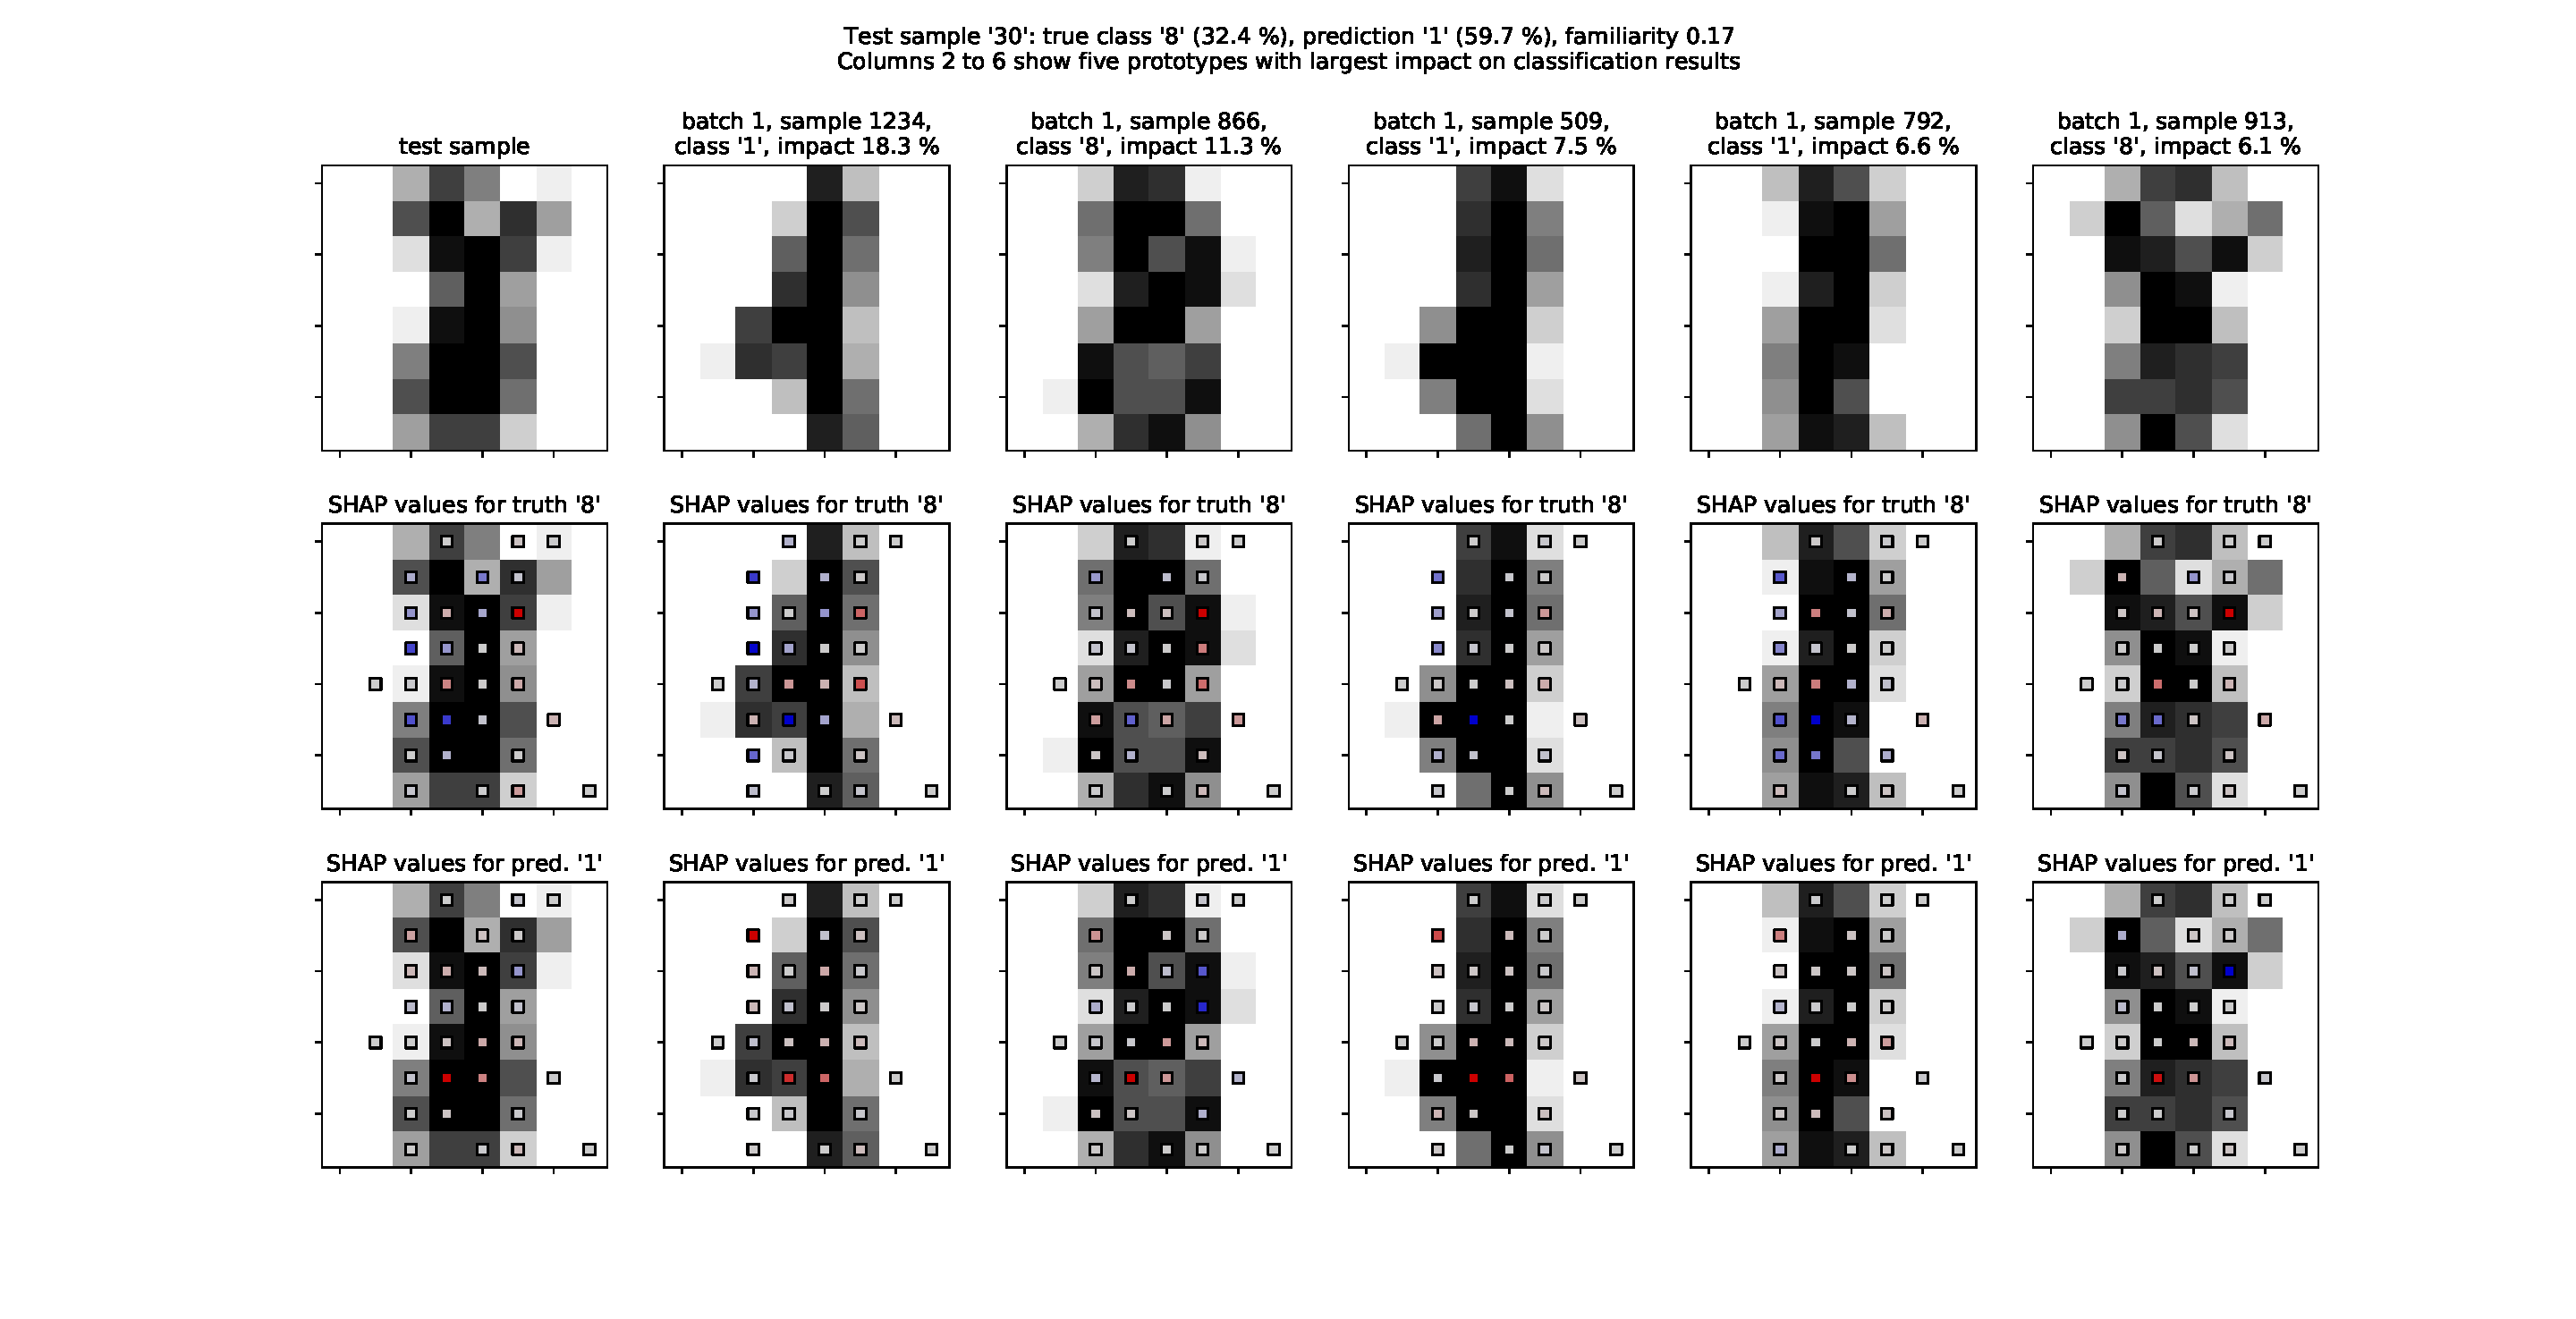
\includegraphics[width=0.9\textheight, angle=90, trim={1.5cm 1.5cm 1.5cm 0.5cm}, clip]{figures/digits_8_vs_1_explanation.pdf}
\end{center}
\end{figure}
%
As a final example, we show how to create an explanation for the digits data set that relies both on prototypes with high impact and SHAP values.
This classification problem is more complex than the one for cancer data.
Figure \ref{fig_batch_1_map_test_digits} presents the `batch 1 map' including test data and a reference point selected using the ranking rule.
Several classes are well differentiated in this plot, but a two-dimensional representation clearly cannot capture the whole structure.\par
%
Figure \ref{fig_impact_shap} is a custom plot for explaining a particular misclassified digit.
It shows the case itself -- an `8' for which the highest probability is estimated for class `1' -- as well as the five prototypes with the largest impact on the result.
The second row overlays the SHAP values for the probability estimate of the true class `8', the third does the same for class `1'.
A red color indicates that the estimate is increased because of the grayscale value of the associated pixel, a blue color that it is decreased.
Note that the estimated probabilities for the baseline are 61 \% for class `8', 27 \% for class `3', and negligible for the other digits.
Thus, the SHAP values indicate the importance of the features for a shift away from this distribution towards 60 \% for class `1' and 32 \% for class `8'.
%
\endinput

\chapter{Implementation notes}
\label{ch_implementation}
%
This chapter provides a brief overview of the code repository for Python module \texttt{proset}, the module's public interface, and some implementation details.
%
\section{Repository structure}
\label{sec_repository}
%
The code repository has the following directory structure:
%
\begin{description}
\item[\texttt{<main directory>:}] configuration files and general information.
%
\item[\texttt{doc:}] the LaTeX source files and images for this document.
%
\item[\texttt{proset:}] the source code for Python module \texttt{proset}.
%
\item[\texttt{scripts:}] Python scripts for the benchmark study.
Each data set has its own subfolder with similar content.
E.g., the subfolder for the iris data contains the following files:
%
\begin{description}
\item[\texttt{iris\_2f\_prepare\_data.py:}] fetch and format the data, apply a 70:30 train-test split, save results to disk.
%
\item[\texttt{iris\_2f\_fit.py:}] load prepared data and fit a proset model using one of several strategies for selecting hyperparameters, save results to disk.
%
\item[\texttt{iris\_2f\_diagnostics.py:}] load fitted proset model, create diagnostic reports and plots.
The script generates all information for proset on iris data reported in Sections \ref{sec_classifier_benchmarks} and \ref{sec_classifier_comparison}.
%
\item[\texttt{iris\_2f\_explain.py:}] load fitted proset model, create explanatory reports and plots.
The script demonstrates the explanatory features discussed in Chapter \ref{ch_explainability}.
%
\item[\texttt{iris\_2f\_knn\_fit.py:}] load prepared data and fit a kNN model with hyperparameter selection, save results to disk.
%
\item[\texttt{iris\_2f\_knn\_diagnostics.py:}] load fitted kNN model, create diagnostic reports and plots.
The script generates all information for kNN on iris data found in Section \ref{sec_classifier_comparison}.
%
\item[\texttt{iris\_2f\_xgb\_fit.py:}] load prepared data and fit an XGBoost model with hyperparameter selection, save results to disk.
%
\item[\texttt{iris\_2f\_xgb\_diagnostics.py:}] load fitted XGBoost model, create diagnostic reports and plots.
The script generates all information for XGBoost on iris data reported in Section \ref{sec_classifier_comparison}.
\end{description}
%
Two additional subfolders \texttt{results} and \texttt{reports} contain only dummy files in the git repository.
They are used by the benchmark scripts to store prepared data, fitted models, and explanatory reports.\par
%
Note that all scripts are set up to run from the parent directory of \texttt{scripts}.
E.g., start data preparation from the iPython console via
%
\begin{center}
\texttt{\%run scripts/iris\_2f/iris\_2f\_prepare\_data.py}
\end{center}
%
\item[test:] unit tests for the \texttt{proset} module.
\end{description}
%
\section{Python module \texttt{proset} -- public interface}
\label{sec_proset_module}
%
This section describes the public interface of module \texttt{proset}.
We do not provide complete call signatures for the functions.
Pythons \texttt{help()} function can be used to obtain these from the docstrings.
%
\begin{description}
\item[\texttt{proset:}] the main module exposes a single class:
%
\begin{description}
\item[\texttt{ClassifierModel:}] the proset classifier has an interface compatible with Python module \texttt{sklearn} \cite{Pedregosa_11}.
Its public methods are
%
\begin{description}
\item[\texttt{\_\_init\_\_():}] initialize a proset classifier with hyperparameters and a random state, see Section \ref{sec_classifier_fit}.
%
\item[\texttt{fit():}] fit proset classifier given a feature matrix and target.
This function can take observation weights as an optional parameter.
It can also perform a warm start, in which case new batches are added to an existing model.
%
\item[\texttt{predict():}] predict classes given a feature matrix.
This function requires the model to be already fitted.
It takes the number of batches for evaluation as optional input and can provide familiarity (see Section \ref{sec_familiarity}) as optional output.\par
%
The prediction is made via the `naive'  rule to return the class with the highest estimated probability for each feature vector.
See the discussion in \ref{sec_shap_values} why this is not suitable for real applications.
We recommend to use \texttt{predict\_proba()} with a problem-specific decision rule instead.
%
\item[\texttt{predict\_proba():}] predict class probabilities given a feature matrix.
This function requires the model to be already fitted.
It has the same optional inputs and outputs as \texttt{predict()}.
%
\item[\texttt{score():}] compute the log-likelihood (not \textit{negative} log-likelihood due to \texttt{sklearn} conventions) for a feature matrix.
This function requires the model to be already fitted.
It takes sample weights as optional input, as well as the number of batches for evaluation.
%
\item[\texttt{export():}] export information on prototypes and parameters from a fitted model.
This function returns a tabular report as a \texttt{pandas} data frame \cite{McKinney_10}.
%
\item[\texttt{explain():}] generate an explanation report for a single sample as described in Section \ref{sec_explanation_report}.
This function returns a tabular report similar to \texttt{export}.
See Figure \ref{fig_explanation_report} for an example.
%
\item[\texttt{shrink():}] reduce a fitted model to take only the features with nonzero weights as input.
The model object gains as property the array \texttt{active\_features\_} containing the indices of active features with respect to the original feature vector.
\end{description}
%
Before the \texttt{fit()} method is called, a \texttt{ClassifierModel} object's only public properties are the hyperparameters passed to \texttt{\_\_init\_\_()}.
After fitting, it gains the following additional properties:
%
\begin{description}
\item[\texttt{n\_features\_in\_}:] the expected number of input features.
%
\item[\texttt{classes\_}:] an array of class labels.
%
\item[\texttt{label\_encoder\_}:] an \texttt{sklearn} label encoder object that maps class labels to the integers from 0 to $K-1$.
%
\item[\texttt{set\_manager\_}:] an instance of the \texttt{SetManager} class that stores information on prototypes and proset model parameters, see Section \ref{sec_implementation} for details.
The \texttt{SetManager} can provide additional information on the model via the following public methods and properties:
%
\begin{description}
\item[\texttt{num\_batches:}] the number of batches.
Note that the fitting procedure does not remove batches with no prototypes, i.e., the model always has the number of batches specified by the user even if some or all of them are empty.
%
\item[\texttt{num\_features:}] the expected number of input features.
%
\item[\texttt{get\_active\_features():}] returns the index vector of active features.
%
\item[\texttt{get\_num\_prototypes():}] returns the total number of prototypes.
Note that the same training sample is counted multiple times if it appears as prototype in multiple batches.
%
\item[\texttt{get\_feature\_weights():}] returns a matrix of the weights of active features for all batches, sorted in descending order of weights, as well as the index vector of features with respect to the original ordering.
%
\item[\texttt{get\_batches():}] export the entire model structure as a Python \texttt{list} of \texttt{dict} objects.
An empty batch is returned as \texttt{None} value instead of a \texttt{dict}.
\end{description}
\end{description}
%
Note that class \texttt{SetManager} has more public methods than listed above, but these are intended for the manipulation of its content via \texttt{fit()}.
%
\end{description}
%
\item[\texttt{proset.utility:}] this submodule contains helper functions for working with proset models:
%
\begin{description}
\item[\texttt{select\_hyperparameters():}] fit a proset model using cross-validation to select hyperparameters.
This function implements Algorithm \ref{alg_hyperparameters}.
%
\item[\texttt{print\_hyperparameter\_report():}] print a summary of hyperparameter selection and quality metrics to the console.
%
\item[\texttt{print\_feature\_report():}] print information about selected features to the console.
%
\item[\texttt{choose\_reference\_point():}] choose a reference point for the SHAP explainer, see Section \ref{sec_shap_values} for details.
This function implements Algorithm \ref{alg_shap_baseline}.
%
\item[\texttt{print\_point\_report():}] print information about a single point to the console.
%
\item[\texttt{plot\_select\_results():}] create plots for hyperparameter search results.
Figure \ref{fig_parameter_search} was created with this function.
%
\item[\texttt{ClassifierPlots:}] helper class used to create most of the diagnostic plots in this document.
See the benchmark scripts for usage examples.
%
\item[\texttt{write\_report():}] save a report created by a proset model's \texttt{export()} or \texttt{explain()} functions to disk as a formatted Excel file.
\end{description}
%
\item[\texttt{proset.benchmarks:}] this submodule contains additional functions for the benchmark study:
%
\begin{description}
\item[\texttt{start\_console\_log():}] invoke \texttt{proset} logging so a progress report for model fitting is printed to the console.
%
\item[\texttt{fit\_knn\_classifier():}] fit a kNN classifier using cross-validation to select $k$.
%
\item[\texttt{fit\_xgb\_classifier():}] fit an XGBoost classifier using cross-validated selection of hyperparameters as discussed in Section \ref{sec_classifier_comparison}.
%
\item[\texttt{print\_xgb\_classifier\_report():}] print a summary of XGBoost hyperparameter selection and quality metrics to the console.
%
\item[\texttt{create\_checkerboard():}] create a sample of checkerboard data, see Section \ref{sec_classifier_benchmarks}.
%
\item[\texttt{create\_continuous\_xor():}] create a sample of `continuous XOR' data, see Section \ref{sec_classifier_benchmarks}.
\end{description}
\end{description}
%
\section{Implementation details}
\label{sec_implementation}
%
The core functionality of proset is implemented as three interdependent classes.
Each exists once as an abstract base class with shared functionality and then as a concrete subclass for each type of estimator:
%
\begin{description}
\item[\texttt{Model:}] implements the public interface of estimators following the conventions established by Python package \texttt{sklearn} \cite{Pedregosa_11}.
It relies on an instance of class \texttt{SetManager} for storing information on the model structure and on an instance of class \texttt{Objective} for parameter fitting.
The solver is algorithm L-BFGS-B \cite{Byrd_95} from Python package \texttt{scipy} \cite{Virtanen_20}.
%
\item[\texttt{SetManager:}] stores information about the proset model structure, i.e., batches, prototypes, prototype weights, and feature weights.
Computes scaled and unscaled versions of estimators like (\ref{eq_pkx}).
%
\item[\texttt{Objective:}] computes the objective function value and gradient for fitting an additional batch of prototypes to an existing proset model.
See (\ref{eq_log_likelihood}), (\ref{eq_l_partial_v}), and (\ref{eq_l_partial_w}) for the expressions belonging to the proset classifier.
The objective relies on an instance of class \texttt{SetManager} to provide distribution estimates for batches that have already been fitted.
\end{description}
%
The implementation relies on Python package \texttt{numpy} \cite{Harris_20} for fast matrix operations.
It also uses some problem-specific solutions to speed up computation:
%
\begin{enumerate}
\item To evaluate the objective function (\ref{eq_log_likelihood}), we need to compute the squared weighted Euclidean distance between every pair of points where one is a sample reserved for scoring and the other a potential prototype.
These distances can be computed using vector-matrix operations as follows:\par
%
Let $X_0\in\R^{N_0\times D}$ and $X_1\in\R^{N_1\times D}$, $N_1,N_2>0$, be the feature matrices corresponding to the points, and let $v\in\R^d$, $v_d\geq0$, be the vector of feature weights.
For $i\in\{0,1\}$, denote the matrices of weighted features and squared weighted features by
%
\begin{align}
Z_i&:=[v_dX_{i,n,d}]_{n,d}&S_i&:=[v_d^2X_{i,n,d}^2]_{n,d}\label{eq_ZiSi}
\end{align}
%
The row sums of $S_i$ are $s_i:=S_i\1_D\in\R^{N_i}$, where $\1_D$ is the vector of ones in $\R^D$.
Now compute
%
\begin{equation}
W:=s_0\1_{N_1}^T-2Z_0Z_1^T+\1_{N_0}s_1^T\in\R^{N_0,N_1}\label{eq_W}
\end{equation}
%
The elements of this matrix are the desired squared weighted distances, i.e.\
%
\begin{equation}
W_{i,j}=\sum_{d=1}^Dv_d^2(X_{0,i,d}-X_{1,j,d})^2\label{eq_Wij}
\end{equation}
%
Note that \texttt{numpy} has functions for adding a row (column) vector to each row (column) of a matrix, so the products $s_0\1_{N_1}^T$ and $\1_{N_0}s_1^T$ do not have to be generated explicitly.
%
\item When storing a batch of prototypes, the \texttt{SetManager} class reduces the feature matrix to the active features and precomputes $Z_1$ and $s_1$ as above.
%
\item The \texttt{Objective} class reduces both feature matrices to the active features, provided the number of active features is less than a fraction of the total.
This limitation is in place as there is a trade-off between the performance gain from smaller matrices and the time required to copy the data.
We found that a threshold of 70 \% improves performance on the digits data set, but the best value may depend on the structure of the data.\par
%
As an additional measure, the latest version of the reduced matrices is cached.
Thus, if L-BFGS-B requests multiple evaluations of the objective or gradient for the same set of active features (not necessarily the exact same feature weights), no additional copy operations are triggered.
\end{enumerate}
%
\endinput

%
\appendix
\cleardoublepage
\phantomsection
\addcontentsline{toc}{chapter}{Bibliography}
\begin{thebibliography}{99}
\bibitem{Fisher_36}
R.\ A.\ Fisher: `The use of multiple measurements in taxonomic problems', Annual Eugenics, vol.\ 7, part II, pp.\ 179--188, 1936.
%
\bibitem{Fix_51}
E.\ Fix, J.\ L.\ Hodges: `Discriminatory Analysis. Nonparametric Discrimination: Consistency Properties', USAF School of Aviation Medicine, Randolph Field, Texas, 1951.
%
\bibitem{Nadaraya_64}
E.\ A.\ Nadaraya: `On Estimating Regression', Theory of Probability and Its Applications, vol.\ 9, issue 1, pp.\ 141--142, 1964.
%
\bibitem{Watson_64}
G.\ S.\ Watson: `Smooth Regression Analysis', Sankhyā: The Indian Journal of Statistics, Series A, vol.\ 26, no.\ 4, pp.\ 359--372, 1964.
%
\bibitem{Hart_68}
P.\ E.\ Hart: `The Condensed Nearest Neighbor Rule', IEEE Transactions on Information Theory, vol.\ 18, pp.\ 515–516, 1968.
%
\bibitem{Hoerl_70}
A.\ E.\ Hoerl, R.\ W. Kennard: 'Ridge Regression: Biased Estimation for Nonorthogonal Problems', Technometrics, vol. 12, no. 1, pp. 55--67, 1970.
%
\bibitem{Devroye_78}
L.\ P.\ Devroye: `The Uniform Convergence of the Nadaraya-Watson Regression Function Estimate', The Canadian Journal of Statistics / La Revue Canadienne de Statistique, vol.\ 6, no.\ 2, pp.\ 179--191, 1978.
%
\bibitem{Aeberhard_92}
S. Aeberhard, D. Coomans, O. de Vel: `Comparison of Classifiers in High Dimensional Settings', Tech. Rep. no. 92-02, Dept. of Computer Science and Dept. of Mathematics and Statistics, James Cook University of North Queensland, 1992. 
%
\bibitem{Byrd_95}
R.\ H.\ Byrd, P.\ Lu, J.\ Nocedal: `A Limited Memory Algorithm for Bound Constrained Optimization', SIAM Journal on Scientific and Statistical Computing, vol.\ 16, issue 5, pp. 1190--1208, 1995.
%
\bibitem{Tibshirani_96}
R.\ Tibshirani: `Regression Shrinkage and Selection via the Lasso', Journal of the Royal Statistical Society, Series B, vol.\ 58, issue 1, pp.\ 267--288, 1996.
%
\bibitem{Ormoneit_99}
D.\ Ormoneit, T.\ Hastie: `Optimal Kernel Shapes for Local Linear Regression', Advances in Neural Information Processing Systems 12 (NIPS), 1999.
%
\bibitem{Hand_01}
D.\ J.\ Hand, R.\ J.\ Till: `A Simple Generalisation of the Area Under the ROC Curve for Multiple Class Classification Problems', Machine Learning, vol.\ 45, pp.\ 171--186, 2001.
%
\bibitem{Haerdle_04}
W.\ Härdle, M.\ Müller, S.\ Sperlich, A.\ Werwatz: `Nonparametric and Semiparametric Models', Springer, 2004.
%
\bibitem{Hall_04}
P.\ Hall, J.\ Racine, Q.\ Li: `Cross-validation and the Estimation of Conditional Probability Densities', Journal of the American Statistical Association, vol.\ 99, issue 468, pp.\ 1015--1026, 2004.
%
\bibitem{Zou_05}
H.\ Zou, T.\ Hastie: `Regularization and variable selection via the elastic net', Journal of the Royal Statistical Society, Series B, vol.\ 37, part 2, pp.\ 301--320, 2005.
%
\bibitem{Andrew_07}
G.\ Andrew, J.\ Gao: `Scalable Training of $L_1$-Regularized Log-Linear Models', Proceedings of the 24 th International Conference on Machine Learning, 2007.
%
\bibitem{Hayfield_08}
T.\ Hayfield, J.\ S.\ Racine: `Nonparametric Econometrics: The np Package', Journal of Statistical Software, vol.\ 27, issue 5, pp. 1--32, 2008.\par
%
Software available: \url{https://cran.r-project.org/web/packages/np}
%
\bibitem{Bontemps_09}
C.\ Bontemps, J.\ S.\ Racine, M.\ Simoni: `Nonparametric vs Parametric Binary Choice Models: An Empirical Investigation', TSE Working Paper Series 09-126, Toulouse School of Economics, 2009.
%
\bibitem{Friedman_10}
J.\ Friedman, T.\ Hastie, R.\ Tibshirani: `Regularization Paths for Generalized Linear Models via Coordinate Descent', Journal of Statistical Software, vol.\ 33, no.\ 1, pp.\ 1--22, 2010.\par
%
Software available: \url{https://cran.r-project.org/web/packages/glmnet}
%
\bibitem{McKinney_10}
W.\ McKinney: `Data Structures for Statistical Computing in Python', Proceedings of the 9th Python Science Conference, pp.\ 56--61, 2010.\par
%
Software available: \url{https://pandas.pydata.org}
%
\bibitem{Pedregosa_11}
F.\ Pedregosa, G.\ Varoquaux, A.\ Gramfort, V.\ Michel, B.\ Thirion, O.\ Grisel, M.\ Blondel, P.\ Prettenhofer, R.\ Weiss, V.\ Dubourg, J.\ Vanderplas, A.\ Passos, D.\ Cournapeau, M.\ Brucher, M.\ Perrot, E.\ Duchesnay: `Scikit-learn: Machine Learning in Python', JMLR 12, pp. 2825--2830, 2011.\par
%
Software available: \url{https://scikit-learn.org}
%
\bibitem{Chen_16}
T.\ Chen, C.\ Guestrin: `XGBoost: A Scalable Tree Boosting System', Proceedings of the 22nd ACM SIGKDD International Conference on Knowledge Discovery and Data Mining, pp. 785--794, 2016.\par
%
Software available: \url{https://xgboost.ai}
%
\bibitem{Lundberg_17}
S.\ M.\ Lundberg, S.-I.\ Lee: `A Unified Approach to Interpreting Model Predictions', Advances in Neural Information Processing Systems 30 (NIPS), 2017.\par
%
Software available: \url{https://shap.readthedocs.io/en/latest/index.html}
%
\bibitem{Lundberg_18}
S.\ M.\ Lundberg, G.\ G.\ Erion, S.-I.\ Lee: `Consistent Individualized Feature Attribution for Tree Ensembles', arXiv:1802.03888, arxiv.org, 2018.
%
\bibitem{Dua_19}
D.\ Dua, C.\ Graff: UCI Machine Learning Repository, Irvine, CA: University of California, School of Information and Computer Science, 2019.\par
%
Data available: \url{https://archive.ics.uci.edu/ml}
%
\bibitem{Harrell_20}
F.\ Harrel: `Classification vs. Prediction', blog article, 2020.\par
%
Available: \url{https://www.fharrell.com/post/classification/}
%
\bibitem{Harris_20}
C.\ R.\ Harris, K.\ J.\ Millman, S.\ J.\ van der Walt, R.\ Gommers, P.\ Virtanen, D.\ Cournapeau, E.\ Wieser, J.\ Taylor, S.\ Berg, N.\ J.\ Smith, R.\ Kern, M.\ Picus, S.\ Hoyer, M.\ H.\ van Kerkwijk, M.\ Brett, A.\ Haldane, J.\ Fern{\'a}ndez del R{\'i}o, M.\ Wiebe, P.\ Peterson, P.\ G{\'e}rard-Marchant, K.\ Sheppard, T.\ Reddy, W.\ Weckesser, H.\ Abbasi, C.\ Gohlke, T.\ E.\ Oliphant: `Array programming with NumPy', Nature, vol.\ 585, pp.\ 357--362, 2020.\par
%
Software available: \url{https://numpy.org/}
%
\bibitem{Izzo_20}
C.\ Izzo, A.\ Lipani, R.\ Okhrati, F.\ Medda: `A Baseline for Shapely Values in MLPs: from Missingness to Neutrality', arXiv:2006.04896, arxiv.org, 2020.
%
\bibitem{Virtanen_20}
P.\ Virtanen, R.\ Gommers, T.\ E.\ Oliphant, M.\ Haberland, T.\ Reddy, D.\ Cournapeau, E.\ Burovski, P.\ Peterson, W.\ Weckesser, J.\ Bright, S.\ J.\ van der Walt, M.\ Brett, J.\ Wilson, K.\ J.\ Millman, N.\ Mayorov, A.\ R.\ J.\ Nelson, E.\ Jones, R.\ Kern, E.\ Larson, C J Carey, {\.I}. Polat, Y.\ Feng, E.\ W. Moore, J.\ VanderPlas, D.\ Laxalde, J.\ Perktold, R.\ Cimrman, I.\ Henriksen, E.\ A.\ Quintero, C.\ R.\ Harris, A.\ M.\ Archibald, A.\ H.\ Ribeiro, F.\ Pedregosa, P.\ van Mulbregt, SciPy 1.0 Contributors: 'SciPy 1.0: Fundamental Algorithms for Scientific Computing in Python', Nature Methods, vol.\ 17, issue 3, pp.\ 261--272, 2020.\par
%
Software available: \url{https://scipy.org/}
%
\bibitem{Leisch_21}
F.\ Leisch, E.\ Dimitriadou: `mlbench: Machine Learning Benchmark Problems', R package, 2021.\par
%
Software available: \url{https://cran.r-project.org/web/packages/mlbench}
\end{thebibliography}
\endinput

\end{document}
